%=================================================================
% MIT LICENSE
%=================================================================
% Copyright (c) 2022 Techneatium
%
% Permission is hereby granted, free of charge, to any person obtaining a copy
% of this software and associated documentation files (the "Software"), to deal
% in the Software without restriction, including without limitation the rights
% to use, copy, modify, merge, publish, distribute, sublicense, and/or sell
% copies of the Software, and to permit persons to whom the Software is
% furnished to do so, subject to the following conditions:
%
% The above copyright notice and this permission notice shall be included in all
% copies or substantial portions of the Software.
%
% THE SOFTWARE IS PROVIDED "AS IS", WITHOUT WARRANTY OF ANY KIND, EXPRESS OR
% IMPLIED, INCLUDING BUT NOT LIMITED TO THE WARRANTIES OF MERCHANTABILITY,
% FITNESS FOR A PARTICULAR PURPOSE AND NONINFRINGEMENT. IN NO EVENT SHALL THE
% AUTHORS OR COPYRIGHT HOLDERS BE LIABLE FOR ANY CLAIM, DAMAGES OR OTHER
% LIABILITY, WHETHER IN AN ACTION OF CONTRACT, TORT OR OTHERWISE, ARISING FROM,
% OUT OF OR IN CONNECTION WITH THE SOFTWARE OR THE USE OR OTHER DEALINGS IN THE
% SOFTWARE.
%=================================================================

%-----------------------------------------------------------------
% BEGIN DOCUMENT
%-----------------------------------------------------------------
\documentclass[fontSpartan]{TechCheck}
\title{F14_Cheatsheet}
\author{Techneatium}

\setaircraftlong{F-14A/B AIRCRAFT} % sets long label for title page
\setaircraftshort{F-14A/B} % sets short label for header
\settabnumber{6} % sets number of tabs for document

% Begin Document

\begin{document}
	%-----------------------------------------------------------------
% TITLE PAGE
%-----------------------------------------------------------------
	% deactivate header and footer
	\pagestyle{empty}
	\newlength{\centeroffset}
	\setlength\centeroffset{(\chevin-\outmar-0.5cm)/2}
	\begin{tikzpicture}[overlay, remember picture]
	\node[
	]() at ([xshift=\centeroffset,yshift=8.5cm]current page.center) {
		\Huge \textbf{Pocket Checklist}
	};
	\node[
	]() at ([xshift=\centeroffset,yshift=7cm]current page.center) {
		\resizebox{10cm}{!}{\textbf{\colorbox{black}{\textcolor{white}{F-14A/B AIRCRAFT}}}}
	};
	\node[
	]() at ([xshift=\centeroffset,yshift=5.5cm]current page.center) {
		\Large \textbf{\colorbox{color1}{\textcolor{white}{REV: \today}}} \blue{}
	};
	\node[
	]() at ([xshift=\centeroffset,yshift=-1cm]current page.center) {
		\includegraphics[
			width=0.8\linewidth,
			page = {1},
			trim = {3cm, 10.5cm, 6.5cm, 13.5cm},
			clip
		]{natops_F14B.pdf}
	};
	% Black area for white chevrons
	\fill[black]
		([xshift=\outmar, yshift=0.2cm]current page text area.north east) --
		([xshift=\outmar, yshift=-\botmar]current page text area.south east) --
		([xshift=\chevin-0.5cm, yshift=-\botmar]current page text area.south east) --
		([xshift=\chevin-0.5cm, yshift=0.2cm]current page text area.north east) --
		cycle;
	\end{tikzpicture}
	% label for hyperrefs back to frontpage
	\label{frontpage}
	% make chevrons
	\thumbfront{Procedures}{0}
	\thumbfront{Systems}{1}
	% use tabular for multi line node
	\thumbfront{\begin{tabular}{c} AWG-9 \\ Radar \end{tabular}}{2}
	\thumbfront{\begin{tabular}{c} TCS \\ LANTIRN \end{tabular}}{3}
	\thumbfront{\begin{tabular}{c} A/G \\ Weapons \end{tabular}}{4}
	\thumbfront{\begin{tabular}{c} A/A \\ Weapons \end{tabular}}{5}
	\thumbwide

	\clearpage
	\null\vspace{0cm}

	\begin{tcolorbox}[
		enhanced, colback=white, colframe=color1, colbacktitle=white, coltitle=color1, sharp corners, attach boxed title to top center={yshift=2mm},
		boxed title style={
			sharp corners,
			drop shadow=color1!100
		}, title=\LARGE\textbf{DISCLAIMER}
	]
		\textbf{This document represents a personal project and is intended for entertainment purposes only. Do not use for training purposes or in real life scenarios.}
	\end{tcolorbox}

	\cleardoublepage

	\pagestyle{empty}
	\dominitoc
	\tableofcontents
	\cleardoublepage

	% restart page counter
	\setcounter{page}{1}
	% reactivate header and footer
	\pagestyle{body}

	\chapter{PROCEDURES}
	\thumbtab{Procedures}{0}
	\minitoc
	\cleardoublepage

	\section{START-UP}

	\subsection{PILOT - PRE-START}
	\begin{tablenumerate}
		\blueitem{Parking Brake}{\textbf{ENGAGED}\cbstart}
		\blueitem{Ground Crew}{
		\begin{subenumerate}
			\item Ground Power \dotfill connected
			\item Compressed Air \dotfill connected
		\end{subenumerate}\cbend}
		\blueitem{ICS}{\textbf{HOT MIC}}
		\dblueitem{TO RIO}{\emph{``Begin Start-Up''}\cbstart}
		\blueitem{ICS}{\textbf{Comm Check}\cbend}
		\blueitem{MASTER TEST \break Selector}{
		\begin{subenumerate}
			\item \textbf{LTS}
			\begin{itemize}
				\item \textbf{Warning Lights} \dotfill checked
				\item \textbf{Caution Lights} \dotfill checked
				\item \textbf{Advisory Lights} \dotfill checked
			\end{itemize}
			\item \textbf{FIRE DET/EXT}
			\begin{itemize}
				\item \textbf{L FIRE GO} \dotfill illuminated
				\item \textbf{R FIRE GO} \dotfill illuminated
			\end{itemize}
			\item \textbf{INST}
			\begin{itemize}
				\item \textbf{RPM} \dotfill 96\%
				\item \textbf{EGT} \dotfill 960 C
				\item \textbf{FF} \dotfill 10500 pph
				\item \textbf{AOA} \dotfill 18 $\pm$ 5
				\item \textbf{Wing Sweep} \dotfill 45 $\pm$ 2.5
				\item \textbf{FUEL QTY} \dotfill 2000 $\pm$ 200
				\item \textbf{Oxygen QTY} \dotfill 2 liters
				\item \textbf{L\&R FF lights} \dotfill illuminated
			\end{itemize}
			\item \textbf{OFF}
		\end{subenumerate}}
		\blueitem{Ejection Seat}{\textbf{Armed}\cbstart}
		\dblueitem{RIO}{Canopy Closed}
		\blueitem{Oxygen}{\textbf{ON (FWD)}}
		\blueitem{Emergency Wing Sweep\cbend}{\textbf{OVERSWEEP}}
	\end{tablenumerate}

	\clearpage

	\subsection{PILOT - ENGINE START}
	\begin{tablenumerate}
		\blueitem{AIR SOURCE}{\textbf{OFF}}
		\blueitem{Hydraulics}{
		\begin{subenumerate}
			\item \textbf{HYD TRANSFER PUMP} \dotfill \textbf{SHUTOFF}
			\item \textbf{Emerg. Hyd.} \dotfill \textbf{AUTO (LOW)}
		\end{subenumerate}}
		\blueitem{L\&R MASTER GEN}{\textbf{NORM}}
		\dblueitem{RIO}{\emph{``Ready to Start''}\cbstart}
		\blueitem{Right Engine \break Start-Up}{
		\begin{subenumerate}
			\item \textbf{Engine Crank} \dotfill \textbf{R}
			\item \textbf{R Eng N2} \dotfill 20\%
			\item \textbf{R Throttle} \dotfill \textbf{IDLE}
			\item \textbf{TIT} \dotfill < 890 C during start
			\item \textbf{R GEN CAUTION} \dotfill extinguished
		\end{subenumerate}\cbend}
		\blueitem{Stabilized \break Parameters}{
		\begin{subitemize}
			\item \textbf{RPM} \dotfill 62-78\%
			\item \textbf{TIT} \dotfill approx 500 C
			\item \textbf{Fuel Flow} \dotfill 950-1400 pph
			\item \textbf{NOZ} \dotfill 5 (100\%)
			\item \textbf{Oil Pressure} \dotfill 25-35 psi
			\item \textbf{Hyd Pressure} \dotfill 3000 psi
		\end{subitemize}}
		\blueitem{Left Engine\cbstart \break Start-Up}{
		\begin{subenumerate}
			\item \textbf{Engine Crank} \dotfill \textbf{L}
			\item \textbf{L Eng N2} \dotfill 20\%
			\item \textbf{L Throttle} \dotfill \textbf{IDLE}
			\item \textbf{TIT} \dotfill < 890 C during start
			\item \textbf{L GEN Caution} \dotfill extinguished
		\end{subenumerate}\cbend}
		\blueitem{Stabilized \break Parameters}{
		\begin{subitemize}
			\item \textbf{RPM} \dotfill 62-78\%
			\item \textbf{TIT} \dotfill approx 500 C
			\item \textbf{Fuel Flow} \dotfill 950-1400 pph
			\item \textbf{NOZ} \dotfill 5 (100\%)
			\item \textbf{Oil Pressure} \dotfill 25-35 psi
			\item \textbf{Hyd Pressure} \dotfill 3000 psi
		\end{subitemize}}
		\blueitem{HYD TRANSFER PUMP}{\textbf{NORM}}
		\blueitem{HYD PRESSURE}{3000 psi}
		\blueitem{AIR SOURCE}{\textbf{BOTH ENG}\cbstart}
		\blueitem{Ground Power}{disconnected}
		\blueitem{Compressed Air}{disconnected\cbend}
	\end{tablenumerate}

	\clearpage

	\subsection{PILOT - POST-START}
	\begin{tablenumerate}
		\dblueitem{TO RIO}{\emph{``Both Engines Running''}}
		\blueitem{Displays \cbstart Control Panel}{
		\begin{subitemize}
			\item \textbf{VDI} \dotfill \textbf{ON}
			\item \textbf{HUD} \dotfill \textbf{ON}
			\item \textbf{HSD} \dotfill \textbf{ON}
			\item \textbf{HDS MODE} \dotfill \textbf{TID}\\
			\hfill (monitor INS)\cbend
		\end{subitemize}}
		\dblueitem{RIO}{\textbf{Select Align Quality}
		\begin{subitemize}
			\item \textbf{INS GO NOW} -- shortest but least precise alignment
			\item \textbf{INS GO COARSE} -- does not meet Launch Criteria for AIM-7 / AIM-54
			\item \textbf{INS GO MIN WPN LAUNCH} -- allows AIM-7 / AIM-54 launch
			\item \textbf{INS GO FINE} -- fine align (8 min)
		\end{subitemize}}
		\blueitem{ACM Panel}{
		\begin{subitemize}
			\item \textbf{GUN RATE} \dotfill as required
			\item \textbf{SW COOL} \dotfill \textbf{OFF}
			\item \textbf{MSL PREP} \dotfill \textbf{OFF}
			\item \textbf{Missile MODE/STP} \dotfill \textbf{NORM}
		\end{subitemize}}
		\blueitem{Gun Rounds}{\textbf{Set}}
		\blueitem{ANTI-SKID SPOILER BK}{\textbf{OFF}}
		\blueitem{Emergency \cbstart Wing Sweep}{
		\begin{subenumerate}
			\item \textbf{Handle} \dotfill \textbf{AFT}
			\item \textbf{Angle} \dotfill Verify 68 deg
		\end{subenumerate}}
		\blueitem{AFCS Panel - SAS STAB AUG}{
		\begin{subitemize}
			\item \textbf{PITCH} \dotfill \textbf{ON}
			\item \textbf{ROLL} \dotfill \textbf{ON}
			\item \textbf{YAW} \dotfill \textbf{ON}
		\end{subitemize}\cbend}
		\blueitem{WING/EXT TRANS}{\textbf{AUTO}}
		\blueitem{UHF 1 \cbstart Function Selector}{\textbf{BOTH}}
		\blueitem{TACAN Function Selector}{\textbf{T/R}}
		\blueitem{ARA-63 ICLS \break RECEIVER\cbend}{\textbf{ON}}
		\blueitem{Radar Altimeter\cbstart}{
		\begin{subenumerate}
			\item \textbf{Control Knob} \dotfill one click CW to turn on
			\item \textbf{Display} \dotfill 6000 ft (warm up)
			\item \textbf{Display} \dotfill 0 ft (ready)
		\end{subenumerate}}
		\blueitem{Standby ADI\cbend}{erect at least 2 min before T/O}
		\blueitem{KY-28 Crypt. Key}{\textbf{Set} (refer to GROUND SETTINGS kb)}
		\dblueitem{RIO\cbstart}{set D/L frequency \cbend}
		\blueitem{Lights}{As desired}
	\end{tablenumerate}

	\warningbox{
	\begin{itemize}
		\item \textbf{PARKING BRAKE MUST BE ENGAGED DURING ALIGNMENT.} \\
		Lack of parking brake engagement inhibits INS alignment
	\end{itemize}
	}

	\cleardoublepage

	\subsection{RIO - PRE-START}
	\begin{tablenumerate}
		\blueitem{Oxygen\cbstart}{\textbf{ON (FWD)}}
		\dblueitem{PILOT}{
		\begin{subitemize}
			\item \textbf{Ground Power} \dotfill connected
			\item \textbf{Compressed Air} \dotfill connected
		\end{subitemize}}
		\blueitem{ICS}{Comm Check\cbend}
		\blueitem{Lights}{As required}
		\blueitem{LTS Test}{Coordinate with Pilot}
		\blueitem{Ejection Seats}{\textbf{ARMED}\cbstart}
		\blueitem{Canopy}{\textbf{CLOSED}}
		\dblueitem{TO PILOT}{\emph{``Ready to Start''}\cbend}
	\end{tablenumerate}

	\subsection{RIO - POST-START - SHORE}
	\begin{tablenumerate}
		\dblueitem{PILOT}{
		\begin{subitemize}
			\item \textbf{Engines} \dotfill started
			\item \textbf{AIR SOURCE} \dotfill BOTH ENG
		\end{subitemize}}
		\blueitem{INS STARTUP\cbstart}{
		\begin{subenumerate}
			\item \textbf{LIQUID COOLING} \dotfill \textbf{ON (FWD)}
			\item \textbf{WCS Switch} \dotfill \textbf{STANDBY}
			\item \textbf{IR/TV Power} \dotfill \textbf{STBY/IR/TV}
			\item \textbf{TID/DDD} \dotfill illuminated after 40 s
		\end{subenumerate}\cbend}
		\blueitem{Kneeboard}{Retrieve Coordinates, Elevation, Magnetic Variation from GROUND SETTINGS Page}
		% \midrule
		% \multicolumn{3}{l}{\blue{WARNING} Input Coords \textbf{BEFORE} selecting \textbf{GND ALIGN} if using ASH} \\
		\blueitem{Start INS Align\cbstart}{
		\begin{subenumerate}
			\item \textbf{Nav Mode} \dotfill \textbf{GND ALIGN}
			\item \textbf{CAP}
			\begin{itemize}
				\item \textbf{Category} \dotfill \textbf{NAV}
				\item \textbf{MESSAGE} \dotfill \textbf{OWN AC}
			\end{itemize}
			\item \textbf{Keyboard}
			\begin{itemize}
				\item \textbf{CLEAR}, \textbf{LAT}, latitude, \textbf{ENTER}
				\item \textbf{LONG}, longitude, \textbf{ENTER}
				\item \textbf{ALT}, altitude, \textbf{ENTER}
			\end{itemize}
			\item \textbf{CAP MESSAGE} \dotfill \textbf{MAG HDG VAR}
			\item \textbf{Keyboard} \dotfill \textbf{HDG}, mag var, \textbf{ENTER}
			\item \textbf{Align Progress} \dotfill Monitor
		\end{subenumerate}}
		\blueitem{U/VHF Mode}{\textbf{T/R G}\cbend}
		\blueitem{Datalink\cbstart}{
		\begin{subenumerate}
			\item \textbf{Kneeboard} \dotfill TACTICAL DL
			\item \textbf{DL Power} \dotfill \textbf{ON (FWD)}
			\item \textbf{DL Mode} \dotfill \textbf{TAC (AFT)}
			\item \textbf{DL Freq.} \dotfill \textbf{Set}
		\end{subenumerate}}
		\blueitem{TACAN}{\textbf{T/R}}
		\blueitem{RWR Panel}{
		\begin{subenumerate}
			\item \textbf{Display Type} \dotfill \textbf{NORM}
			\item \textbf{PWR} \dotfill \textbf{ON}
			\item \textbf{TEST} \dotfill \textbf{SPL}
			\item \textbf{MODE} \dotfill \textbf{LMT}
		\end{subenumerate}}
		\blueitem{DECM}{\textbf{STBY}, then \textbf{ACT}}
		\blueitem{IFF}{
		\begin{subenumerate}
			\item \textbf{MASTER} \dotfill \textbf{STBY}
			\item \textbf{CODE} \dotfill as required
		\end{subenumerate}}
		\blueitem{Altimeter}{Reset\cbend}
		\blueitem{CAP}{Enter Data (WP, FP, \emph{etc.})}
		\blueitem{Displays\cbstart}{
		\begin{subitemize}
			\item \textbf{DDD} \dotfill Set
			\item \textbf{TID} \dotfill Set
			\item \textbf{Multiple Display Indicator} \dotfill Set
		\end{subitemize}\cbend}
		\blueitem{Hand Control Panel}{Set}
		\blueitem{AN/ALE-39\cbstart}{Set (as required)
		\begin{subitemize}
			\item \textbf{AUTO (CHAFF)/MAN}
			\item \textbf{MAN}
		\end{subitemize}}
		\blueitem{Flare Mode}{\textbf{PILOT}}
		\blueitem{Complete INS Align}{
		\begin{subitemize}
			\item \textbf{Duration Full Fine} \dotfill 8 min
			\item \textbf{Duration ASH} \dotfill much faster
		\end{subitemize}

		\begin{subenumerate}
			\item \textbf{Align Complete} \dotfill Caret $\to$ Diamond
			\item \textbf{NAV Mode} \dotfill \textbf{INS NAV}
		\end{subenumerate}}
		\blueitem{Standby ADI}{Erect at least 2 min before T/O}
		\dblueitem{TO PILOT}{\emph{``Ready to Taxi''}\cbend}
		\midrule
		\multicolumn{3}{l}{\textbf{Once Airborne}} \\
		\blueitem{IR/TV Power\cbstart}{\textbf{ON}}
		\blueitem{WCS Switch}{\textbf{WCS XMT}\cbend}
	\end{tablenumerate}

	\clearpage

	\subsection{RIO - POST-START - CARRIER}
	\begin{tablenumerate}
		\dblueitem{PILOT}{
		\begin{subitemize}
			\item \textbf{Engines} \dotfill started
			\item \textbf{AIR SOURCE} \dotfill BOTH ENG
		\end{subitemize}}
		\blueitem{INS STARTUP\cbstart}{
		\begin{subenumerate}
			\item \textbf{LIQUID COOLING} \dotfill \textbf{ON (FWD)}
			\item \textbf{WCS Switch} \dotfill \textbf{STANDBY}
			\item \textbf{IR/TV Power} \dotfill \textbf{STBY/IR/TV}
			\item \textbf{TID/DDD} \dotfill illuminated after 40 s
		\end{subenumerate}}
		\blueitem{Datalink}{
		\begin{subenumerate}
			\item \textbf{Kneeboard} \dotfill TACTICAL DL
			\item \textbf{DL Power} \dotfill \textbf{ON (FWD)}
		\end{subenumerate}}
		\blueitem{Start INS Align}{
		\begin{subenumerate}
			\item \textbf{DL FREQ} \dotfill Set
			\item \textbf{DL Mode} \dotfill \textbf{CAINS/WAYPT}
			\item \textbf{Nav Mode} \dotfill \textbf{CVA}
		\end{subenumerate}}
		\blueitem{U/VHF Mode}{\textbf{T/R G}}
		\blueitem{TACAN}{\textbf{T/R}}
		\blueitem{RWR Panel}{
		\begin{subenumerate}
			\item \textbf{Display Type} \dotfill \textbf{NORM}
			\item \textbf{PWR} \dotfill \textbf{ON}
			\item \textbf{TEST} \dotfill \textbf{SPL}
			\item \textbf{MODE} \dotfill \textbf{LMT}
		\end{subenumerate}}
		\blueitem{DECM}{\textbf{STBY}, then \textbf{ACT}}
		\blueitem{IFF}{
		\begin{subenumerate}
			\item \textbf{MASTER} \dotfill \textbf{STBY}
			\item \textbf{CODE} \dotfill as required
		\end{subenumerate}}
		\blueitem{Altimeter}{Reset\cbend}
		\blueitem{CAP}{Enter Data (WP, FP, \emph{etc.})}
		\blueitem{Displays\cbstart}{
		\begin{subitemize}
			\item \textbf{DDD} \dotfill Set
			\item \textbf{TID} \dotfill Set
			\item \textbf{Multiple Display Indicator} \dotfill Set
		\end{subitemize}\cbend}
		\blueitem{Hand Control Panel}{Set}
		\blueitem{AN/ALE-39\cbstart}{Set (as required)
		\begin{subitemize}
			\item \textbf{AUTO (CHAFF)/MAN}
			\item \textbf{MAN}
		\end{subitemize}}
		\blueitem{Flare Mode}{\textbf{PILOT}\cbend}
		\blueitem{Complete \cbstart INS Align}{
		\begin{subitemize}
			\item \textbf{Duration Full Fine} \dotfill 9 min
			\item \textbf{Duration ASH} \dotfill much faster
		\end{subitemize}

		\begin{subenumerate}
			\item \textbf{Align Complete} \dotfill Caret $\to$ Diamond
			\item \textbf{NAV Mode} \dotfill \textbf{INS NAV}
		\end{subenumerate}}
		\blueitem{Datalink}{
		\begin{subenumerate}
			\item \textbf{DL Mode} \dotfill \textbf{TAC (AFT)}
			\item \textbf{DL Freq.} \dotfill \textbf{Set}
		\end{subenumerate}}
		\blueitem{Standby ADI}{Erect at least 2 min before T/O}
		\dblueitem{TO PILOT}{\emph{``Ready to Taxi''}\cbend}
		\midrule
		\multicolumn{3}{l}{\textbf{Once Airborne}} \\
		\blueitem{IR/TV Power\cbstart}{\textbf{ON}}
		\blueitem{WCS Switch}{\textbf{WCS XMT}\cbend}
	\end{tablenumerate}

	\warningbox{
	\begin{itemize}
		\item Input Coords \textbf{BEFORE} selecting \textbf{GND ALIGN} if using ASH. Else alignment can progress too far to correct coordinates by the time they are input.
		\item \textbf{PARKING BRAKE MUST BE ENGAGED DURING ALIGNMENT.} \\
		Lack of parking brake engagement inhibits INS alignment
	\end{itemize}
	}

	\cleardoublepage

	\section{TAKEOFF \& LANDING}

	\subsection{PRE-TAXI}
	\begin{tablenumerate}
		\blueitem{ANTI-SKID SPOILER BK}{\textbf{OFF}  }
		\blueitem{HOOK BYPASS}{As Required}
		\blueitem{Nose Strut}{\textbf{RETRACTED}}
		\blueitem{HUD MODE}{\textbf{TO}}
		\blueitem{Parking Brake}{\textbf{Released (IN)}}
		\blueitem{NWS}{\textbf{ENGAGED}}
		\blueitem{Path}{verify clear}
	\end{tablenumerate}

	\subsection{TAKEOFF - SHORE}
	\begin{tablenumerate}
		\multicolumn{3}{c}{\textbf{After Lining Up On Runway}} \\
		\midrule
		\blueitem{Wing Sweep}{
		\begin{subenumerate}
			\item \textbf{EM WING SWEEP} \dotfill \textbf{FWD}, then \textbf{IN}
			\item \textbf{MASTER RESET} \dotfill \textbf{PRESS}
			\item \textbf{Wings } \dotfill Verify thumb controller
			\item \textbf{WING SWEEP} \dotfill \textbf{AUTO}
			\item \textbf{Wings} \dotfill Verify at 20 deg
		\end{subenumerate}}
		\blueitem{ANTI SKID SPOILER BK}{\textbf{BOTH (UP)}}
		\blueitem{FLAPS}{\textbf{UP}}
		\blueitem{Trim}{0 deg}
		\blueitem{NWS}{\textbf{DISENGAGED}}
		\blueitem{Takeoff}{
		\begin{subenumerate}
			\item \textbf{Throttle} \dotfill \textbf{MIL} (90\% RPM)
			\item \textbf{Stick} \dotfill \textbf{Back} at 130 KIAS
			\item \textbf{Rotation} \dotfill approx 140 KIAS
			\item \textbf{GEAR} \dotfill \textbf{UP} < 250 KIAS
		\end{subenumerate}}
	\end{tablenumerate}

	\vfill\null
	\clearpage

	\subsection{TAKEOFF - CARRIER}
	\begin{tablenumerate}
		& \blue{Lineup} &
		\begin{subitemize}
			\item Wait behind JBD until Catapult is clear
			\item Follow Taxi Directors Instructions to line up on Catapult
		\end{subitemize} \\
		\blueitem{Wing Sweep}{
		\begin{subenumerate}
			\item \textbf{EM WING SWEEP} \dotfill \textbf{FWD}, then \textbf{IN}
			\item \textbf{MASTER RESET} \dotfill \textbf{PRESS}
			\item \textbf{Wings } \dotfill Verify thumb controller
			\item \textbf{WING SWEEP} \dotfill \textbf{AUTO}
			\item \textbf{Wings} \dotfill Verify at 20 deg
		\end{subenumerate}}
		\blueitem{FLAPS}{\textbf{DOWN}}
		\blueitem{Launch Bar Preparation}{
		\begin{subenumerate}
			\item \textbf{Nose Strut} \dotfill \textbf{KNEEL} when directed
			\item \textbf{Throttle} \dotfill \textbf{UP} when directed
			\item \textbf{Taxi} \dotfill launch bar into shuttle
			\item \textbf{Throttle} \dotfill \textbf{IDLE} when directed
		\end{subenumerate}}
		\blueitem{Trim}{2-3 deg nose up}
		\blueitem{Speed Brakes}{\textbf{IN}}
		\blueitem{Final Checks}{
		\begin{subenumerate}
			\item \textbf{Throttle} \dotfill \textbf{MIL} when directed
			\item \textbf{Control Wipeout}
			\begin{itemize}
				\item Stick Full Forward
				\item Stick Full Aft
				\item Stick Full Left
				\item Stick Full Right
				\item Rudder Full Left
				\item Rudder Full Right
			\end{itemize}
			\item \textbf{Eng. Inst.} \dotfill \textbf{Checked}
			\item \textbf{Caution/Warnings}  \dotfill\textbf{None}
		\end{subenumerate}}
		\blueitem{Catapult Shot}{
		\begin{subenumerate}
			\item \textbf{Salute} \dotfill \textbf{CAT SHOT}
			\item \textbf{Gear} \dotfill \textbf{UP} < 250 KIAS
			\item \textbf{Flaps} \dotfill \textbf{UP} < 225 KIAS
		\end{subenumerate}}
		\blueitem{Clearing Turn}{}
	\end{tablenumerate}

	\subsection{LANDING - OVERHEAD PATTERN}
	\begin{center}
		\resizebox{0.75\linewidth}{!}{
			\includegraphics[
			page = {384},
			trim = {2.5cm, 7.5cm, 2.5cm, 7.5cm},
			clip
			]{natops_F14B.pdf}
		}
	\end{center}

	\begin{tablenumerate}
		\blueitem{Initial Approach}{
		\begin{subitemize}
			\item \textbf{WING SWEEP} \dotfill \textbf{68 deg}
			\item \textbf{HOOK} \dotfill \textbf{DOWN}
			\item \textbf{SAS} \dotfill \textbf{ON}
			\item \textbf{HUD} \dotfill \textbf{LDG}
			\item \textbf{Airspeed} \dotfill \textbf{300-350 KIAS}
			\item \textbf{Altitude} \dotfill \textbf{800 ft}
		\end{subitemize}}
		\blueitem{Initial Break}{
		\begin{subitemize}
			\item \textbf{Break Interval} \dotfill \textbf{15-17 s}
			\item \textbf{BANK} \dotfill \textbf{45-60 deg}
			\item \textbf{SPEED BRAKE} \dotfill \textbf{EXTEND}
			\item \textbf{Throttle} \dotfill \textbf{IDLE}
			\item \textbf{G} \dotfill \textbf{3-4 G}
			\item \textbf{Altitude} \dotfill \textbf{800 ft}
		\end{subitemize}}
		\blueitem{Break Turn}{
		\begin{subitemize}
			\item \textbf{Wing Sweep} \dotfill \textbf{AUTO} < 280 KIAS
			\item \textbf{Landing Gear} \dotfill \textbf{DOWN} < 280 KIAS
			\item \textbf{FLAPS} \dotfill \textbf{DOWN} < 225 KIAS
		\end{subitemize}}
		\blueitem{Downwind}{
		\begin{subitemize}
			\item \textbf{DLC} \dotfill \textbf{Selected} once flaps out
			\item \textbf{AOA} \dotfill \textbf{ON-SPEED}
			\item \textbf{LANDING CHECKLIST}
			\item \textbf{Altitude} \dotfill descend to \textbf{600 ft}
		\end{subitemize}}
		\blueitem{Final Turn}{\textbf{180 Deg Position}
		\begin{subitemize}
			\item \textbf{Abeam Pos.} \dotfill \textbf{1-1.2 nmi}
		\end{subitemize}
		\textbf{90 Deg Position}
		\begin{subitemize}
			\item \textbf{AOA} \dotfill \textbf{DONUT}
			\item \textbf{Altitude} \dotfill \textbf{400-500 ft}
		\end{subitemize}}
		\blueitem{Intercept Glideslope}{
		\begin{subitemize}
			\item \textbf{Distance} \dotfill \textbf{3/4 Mile}
			\item \textbf{Altitude} \dotfill \textbf{360 ft}
			\item \textbf{AOA} \dotfill \textbf{ON-SPEED}
		\end{subitemize}}
	\end{tablenumerate}

	\subsection{LANDING - CHECKLIST}
	\begin{tablenumerate}
		\blueitem{Wing Sweep}{\textbf{20 deg AUTO}}
		\blueitem{Wheels}{
		\begin{subitemize}
			\item \textbf{Lights} \dotfill \textbf{3 DOWN}
			\item \textbf{Transition Light} \dotfill \textbf{OUT}
		\end{subitemize}}
		\blueitem{SAS}{\textbf{ON}}
		\blueitem{FLAPS}{\textbf{DOWN}}
		\blueitem{DLC}{\textbf{Checked}}
		\blueitem{Hook}{
		\begin{subitemize}
			\item \textbf{HOOK} \dotfill \textbf{DOWN}
			\item \textbf{Transition Light} \dotfill \textbf{OUT}
		\end{subitemize}}
		\blueitem{Harness}{\textbf{Locked}}
		\blueitem{Speedbrakes}{\textbf{EXT}}
		\blueitem{Brakes}{\textbf{Check}}
		\blueitem{Fuel}{\textbf{Check}}
	\end{tablenumerate}

	\clearpage

	\section{IN-FLIGHT}
	\subsection{AERIAL REFUELING}
	\begin{tablenumerate}
		\blueitem{REFUELING CHECKLIST}{
		\begin{subenumerate}
			\item \textbf{WCS} \dotfill \textbf{STBY}
			\item \textbf{ARMING} \dotfill \textbf{SAFE}
			\item \textbf{DUMP Switch} \dotfill \textbf{OFF}
			\item \textbf{AIR SOURCE} \dotfill \textbf{L ENG}
			\item \textbf{REFUEL PROBE} \dotfill \textbf{As desired} \\
			\hfill (transition light off)
			\item \textbf{WING SWEEP} \dotfill \textbf{As desired}
		\end{subenumerate}}
		\blueitem{DISENGAGEMENT}{
		\begin{subenumerate}
			\item \textbf{REFUEL PROBE} \dotfill \textbf{RET} \\
			\hfill (transition light off)
			\item \textbf{AIR SOURCE} \dotfill \textbf{BOTH}
			\item \textbf{WING SWEEP} \dotfill \textbf{AUTO}
		\end{subenumerate}}
	\end{tablenumerate}

	\clearpage

	\section{EMERGENCY PROCEDURES}

	\subsection{AIRSTART}
	\begin{tableitemize}
		\blueitem{Spooldown}{\emph{Before significant spooldown}
		\begin{subenumerate}
			\item \textbf{Non-Running ENG} \dotfill \textbf{IDLE} or above
		\end{subenumerate}

		\emph{If no relight occurs}
		\begin{subenumerate}[start=2]
			\item \textbf{Non-Running ENG} \dotfill \textbf{OFF} then \textbf{IDLE}
		\end{subenumerate}

		\emph{If still no relight occurs}
		\begin{subenumerate}[start=3]
			\item \textbf{ENG MODE} \dotfill \textbf{SEC}
			\item \textbf{Non-Running ENG} \dotfill \textbf{OFF} then \textbf{IDLE}
		\end{subenumerate}}
		\blueitem{Cross-Bleed Restart}{
		\emph{With one ENG running, if Spooldown fails}
		\begin{subenumerate}
			\item \textbf{Non-Running ENG} \dotfill \textbf{OFF}
			\item \textbf{FUEL SHUT OFF} \dotfill check
			\item \textbf{Running throttle} \dotfill 80\%+
			\item \textbf{BACK UP IGNITION} \dotfill \textbf{ON}
			\item \textbf{ENG CRANK} \dotfill non-running eng
			\item \textbf{Non-Running ENG} \dotfill \textbf{IDLE}
		\end{subenumerate}

		\emph{If no start occurs}
		\begin{subenumerate}[start=7]
			\item \textbf{Non-Running ENG} \dotfill \textbf{OFF} then \textbf{IDLE}
		\end{subenumerate}

		\emph{If still no start}
		\begin{subenumerate}[start=8]
			\item \textbf{ENG MODE} \dotfill \textbf{SEC}
			\item \textbf{Non-Running ENG} \dotfill \textbf{OFF} then \textbf{IDLE}
		\end{subenumerate}}
		\blueitem{Windmill Restart}{
		\begin{subenumerate}
			\item \textbf{Airspeed} \dotfill >450 kts
			\item \textbf{Throttle} \dotfill IDLE or above
			\item \textbf{BACK UP IGNITION} \dotfill ON
		\end{subenumerate}

		\emph{If no relight occurs}
		\begin{subenumerate}[start=4]
			\item \textbf{Throttle} \dotfill OFF then IDLE
		\end{subenumerate}

		\emph{If still no relight}
		\begin{subenumerate}[start=5]
			\item \textbf{ENG MODE} \dotfill SEC
			\item \textbf{Throttle} \dotfill OFF then IDLE
		\end{subenumerate}}
		\blueitem{Post Restart}{
		\begin{subenumerate}
				\item \textbf{BACK UP IGNITION} \dotfill OFF
				\item \textbf{ENG MODE} \dotfill PRI
			\end{subenumerate}}
	\end{tableitemize}

	\cleardoublepage

	\chapter{SYSTEMS}
	\thumbtab{Systems}{1}
	\minitoc
	\cleardoublepage

	\section{FLIGHT CONTROL SYSTEMS}
	\subsection{AFCS - SAS}
	\begin{tableitemize}
		\blueitem{SAS}{
		\begin{subitemize}
			\item \textbf{Stability Augmentation System}
			\begin{itemize}
				\item \textbf{Not Fly-by-Wire}
				\item Automatic control surface commands generated by analog computer to improve stability
			\end{itemize}
		\end{subitemize}}
		\blueitem{Controls}{
		\begin{subitemize}
			\item \textbf{Three individual Switches}
			\begin{itemize}
				\item Pitch
				\item Roll
				\item Yaw
			\end{itemize}
		\end{subitemize}}
		\blueitem{Autopilot Emergency Disengage Paddle}{
		\begin{subitemize}
			\item \textbf{Paddle on Stick}
			\begin{itemize}
				\item Disengages Autopilot Modes
				\item Deactivates Pitch, Roll SAS Channels
			\end{itemize}
		\end{subitemize}}
	\end{tableitemize}

	\subsection{AFCS - AUTOPILOT}
	\begin{tableitemize}
		\blueitem{Attitude Hold}{
		\begin{subitemize}
			\item \textbf{Basic Attitude Hold}
			\begin{itemize}
				\item Maintains existing pitch \& roll
				\item Attitude can be changed with stick input
				\item If engaged outside limits will automatically move within range
			\end{itemize}
			\item \textbf{Limits}
			\begin{itemize}
				\item Pitch: 30 deg
				\item Roll: 60 deg
			\end{itemize}
			\item \textbf{Engagement}
			\begin{enumerate}
				\item \textbf{SAS Switches} \dotfill \textbf{ON (FWD)}
				\item \textbf{Alt. Hold Mode} \dotfill \textbf{OFF}
				\item \textbf{VEC/PCD/ACL} \dotfill \textbf{OFF}
				\item \textbf{Heading Mode} \dotfill \textbf{OFF}
				\item \textbf{Autopilot Switch} \dotfill \textbf{ENGAGE (FWD)}
			\end{enumerate}
		\end{subitemize}}
		\blueitem{Altitude Hold}{
		\begin{subitemize}
			\item \textbf{Barometric Altitude Hold}
			\begin{itemize}
				\item Maintains current barometric altitude
			\end{itemize}
			\item \textbf{Limits}
			\begin{itemize}
				\item Vertical velocity: < 100 ft/s
			\end{itemize}
			\item \textbf{Engagement}
			\begin{enumerate}
				\item \textbf{SAS Switches} \dotfill \textbf{ON (FWD)}
				\item \textbf{Autopilot Switch} \dotfill \textbf{ENGAGE (FWD)}
				\item \textbf{Alt. Hold Mode} \dotfill \textbf{ALT (FWD)}
				\item \textbf{A/P REF Light} \dotfill Wait until appears
				\item \textbf{NWS Button} \dotfill \textbf{Press}
			\end{enumerate}
		\end{subitemize}}
		\blueitem{Heading Hold}{
		\begin{subitemize}
			\item \textbf{Magnetic Heading Hold}
			\begin{itemize}
				\item Maintains current magneatic heading
			\end{itemize}
			\item \textbf{Limits}
			\begin{itemize}
				\item Bank angle < 5 deg
			\end{itemize}
			\item \textbf{Engagement}
			\begin{enumerate}
				\item \textbf{SAS Switches} \dotfill \textbf{ON (FWD)}
				\item \textbf{Autopilot Switch} \dotfill \textbf{ENGAGE (FWD)}
				\item \textbf{Heading Mode} \dotfill \textbf{HDG (FWD)}
			\end{enumerate}
		\end{subitemize}}
		\blueitem{Ground Track}{
		\begin{subitemize}
			\item \textbf{Autopilot follows ground track}
			\begin{itemize}
				\item Similar to heading hold
				\item Compensates for wind drift
				\item Uses INS data instead of mag. bearing
			\end{itemize}
			\item \textbf{Limits}
			\begin{itemize}
				\item Bank angle < 5 deg
			\end{itemize}
			\item \textbf{Engagement}
			\begin{enumerate}
				\item \textbf{SAS Switches} \dotfill \textbf{ON (FWD)}
				\item \textbf{Autopilot Switch} \dotfill \textbf{ENGAGE (FWD)}
				\item \textbf{Heading Mode} \dotfill \textbf{GT (AFT)}
				\item \textbf{A/P REF Light} \dotfill Wait until appears
				\item \textbf{NWS Button} \dotfill \textbf{Press}
			\end{enumerate}
		\end{subitemize}}
		\blueitem{VEC/PCD}{
		\begin{subitemize}
			\item \textbf{Vector / Precision Course Direction}
			\begin{itemize}
				\item Allows Link 4 controller to remotely direct the aircraft
				\item \textbf{Not Modelled in DCS}
			\end{itemize}
		\end{subitemize}}
		\blueitem{ACL}{
		\begin{subitemize}
			\item \textbf{Automatic Carrier Landing}
			\begin{itemize}
				\item See relevant section
			\end{itemize}
		\end{subitemize}}
		\blueitem{Autopilot Emergency Disengage Paddle}{
		\begin{subitemize}
			\item \textbf{Paddle on Stick}
			\begin{itemize}
				\item \textbf{Disengages Autopilot Modes}
				\item \textbf{Deactivates Pitch, Roll SAS Channels}
			\end{itemize}
		\end{subitemize}}
	\end{tableitemize}

	\subsection{APC / AUTOTHROTTLE}
	\begin{tableitemize}
		\blueitem{APC}{
		\begin{subitemize}
			\item \textbf{Approach Power Compensator}
			\begin{itemize}
				\item Automatic throttle control
				\item \textbf{Maintains ON SPEED AoA}
			\end{itemize}
		\end{subitemize}}
		\blueitem{Conditions}{Inhibited / disengaged if conditions not met:

		\begin{subitemize}
			\item \textbf{Throttles} \dotfill 75\%-90\% RPM
			\item \textbf{Landing Gear Handle}  \dotfill \textbf{Down}
			\item \textbf{Weight on Wheels} \dotfill \textbf{No}
		\end{subitemize}}
		\blueitem{Engage}{
		\begin{subitemize}
			\item \textbf{Throttle Mode} \dotfill \textbf{AUTO (FWD)}
		\end{subitemize}}
		\blueitem{Disengage}{\textbf{Cage/Seam Button}}
	\end{tableitemize}

	\subsection{ACLS}

	\subsection{WING-SWEEP}
	\begin{tableitemize}
		\blueitem{Overview}{
		\begin{subitemize}
			\item \textbf{In Flight Limited between 20 deg \& 68 deg}
			\item \textbf{On Ground can Oversweep to 75 deg}
			\item \textbf{Hydromechanically Controlled}
			\begin{itemize}
				\item Automatically through CADC
				\item Manually with emergency wing-sweep handle
			\end{itemize}
			\item \textbf{15 deg/s at 1g loading}
			\item \textbf{Mechanically linked to ensure symmetry}
		\end{subitemize}}
		\blueitem{CADC Modes}{
		\begin{subitemize}
			\item \textbf{AUTO}
			\begin{itemize}
				\item CADC controls wing position as function of current Mach via wing-sweep program
			\end{itemize}
			\item \textbf{MAN}
			\begin{itemize}
				\item Pilot manually chooses desired wing sweep angle with thumb controller
			\end{itemize}
			\item \textbf{BOMB}
			\begin{itemize}
				\item Sets wing sweep to \textbf{55 deg} or further aft
			\end{itemize}
		\end{subitemize}}
		\blueitem{Emergency Mode}{
		\begin{subitemize}
			\item \textbf{Emergency Wing-Sweep Handle}
			\begin{itemize}
				\item Moved with wing sweep program by spider detent under normal operation
				\item Can be forced out of spider detent and moved manually
			\end{itemize}
		\end{subitemize}}
		\blueitem{Oversweep}{
		\begin{subitemize}
			\item \textbf{Selected via Emergency Wing-Sweep Handle}
			\begin{enumerate}
				\item \textbf{Em. Wing-Sweep} \dotfill \textbf{68 deg} \\
				\hfill Wait for wing-seal airbags to deflate
				\item \textbf{HZ TAIL AUTH} \dotfill \textbf{Illuminated}
				\item \textbf{Em. Wing-Sweep} \dotfill \textbf{75 deg}
			\end{enumerate}
		\end{subitemize}}
		\blueitem{Return to CADC Control}{
		\begin{subitemize}
			\item \textbf{After Emergency Mode / Oversweep}
			\begin{enumerate}
				\item \textbf{Em. Wing-Sweep} \dotfill \textbf{Spider Detent} \\
				\hfill (Fwd on startup)
				\item \textbf{MASTER RESET} \dotfill \textbf{Press}
			\end{enumerate}
		\end{subitemize}}
	\end{tableitemize}

	\begin{center}
		\begin{tabular}{p{3cm} | p{5cm}}
			\toprule
			\textbf{Indicated Mach} & \textbf{Max Forward Wing Position} \\
			\midrule
			0.4 & 20 deg \\
			\midrule
			0.7 & 25 deg \\
			\midrule
			0.8 & 50 deg \\
			\midrule
			0.9 & 60 deg \\
			\midrule
			1.0 & 68 deg \\
			\bottomrule
		\end{tabular}
	\end{center}

	\notebox{
		\begin{itemize}
			\item Indicates \textbf{Max} forward selectable wing sweep position
		\end{itemize}
	}

	\clearpage

	\section{NAVIGATION SYSTEMS}

	\subsection{OVERVIEW}
	\begin{tableitemize}
		\blueitem{CAINS}{\textbf{C}arrier \textbf{A}ircraft \textbf{I}nertial \textbf{N}avigation \textbf{S}ystem
		\begin{subitemize}
			\item \textbf{Primary navigation system of F-14}
			\item Additionally provides information for tactical systems
			\begin{itemize}
				\item Own position for long-range AIM-7 \& AIM-54 modes
				\item Accurate Datalink sharing/receiving
			\end{itemize}
		\end{subitemize}}
		\midrule
		\multicolumn{3}{c}{\blue{Main Components}} \\
		\blueitem{IMU}{\textbf{I}nertial \textbf{M}easurement \textbf{U}nit
		\begin{subitemize}
			\item 3-Axis, 4-Gimbal system prevents gimbal-lock
			\item 2 gyros provide aircraft attitude and stabilize the platform
			\item 3 accelerometers measure accelerations in all orthogonal axes
		\end{subitemize}}
		\blueitem{CSDC}{\textbf{C}omputer \textbf{S}ignal \textbf{D}ata \textbf{C}onverter
		\begin{subitemize}
			\item Handles data interface between sensors and \textbf{WCS}
		\end{subitemize}}
		\blueitem{WCS}{\textbf{AWG-9 Computer}
		\begin{subitemize}
			\item \textbf{WCS} performs general navigation computations and provides them to PILOT \& RIO through displays
		\end{subitemize}}
		\blueitem{NPS}{ \textbf{N}avigation \textbf{P}ower \textbf{S}upply
		\begin{subitemize}
			\item Provides power to \textbf{IMU} \& \textbf{CSDC}
		\end{subitemize}}
		\blueitem{Subsystems}{
		\begin{subitemize}
			\item Radar Altimeter
			\item TACAN
			\item AHRS
		\end{subitemize}}
		\midrule
		\multicolumn{3}{c}{\blue{Controls}} \\
		\blueitem{CAP}{
		\begin{subitemize}
			\item Used for Data Entry
			\item \textbf{CATEGORY} -- \textbf{NAV}
		\end{subitemize}}
		\blueitem{NAV MODE Selector}{
		\begin{subitemize}
			\item \textbf{OFF} -- Turns off power to IMU
			\item \textbf{ALIGN} -- Three align modes \\
			\hfill \hyperref[subsec:align-nonsat]{\textbf{See Alignment Section}}
			\item \textbf{INS} -- Selects normal INS navigation mode
			\item \textbf{IMU/AM} -- Selects backup mode. Uses IMU for aircraft attitude, TAS from CADC, and stored/entered winds for navigation
			\item \textbf{AHRS/AM} -- Selects further degraded backup mode. Uses magnetic heading from AHRS, TAS and AoA from CADC, and stored wind and mag var for navigation
		\end{subitemize}}
		\midrule
		\multicolumn{3}{c}{\blue{Failure Indicators}} \\
		\blueitem{NAV COMP Light}{
		\begin{subitemize}
			\item If illuminates while \textbf{NAV MODE} is in \textbf{INS} indicates failure in \textbf{INS} or \textbf{CSDC}
			\item Navigation system automatically switches to \textbf{IMU/AM}
			\item Remains illuminated until \textbf{NAV MODE} is set to \textbf{IMU/AM}
		\end{subitemize}}
		\blueitem{IMU Light}{
		\begin{subitemize}
			\item Indicates failure of \textbf{IMU}
			\item Navigation system automatically switches to \textbf{AHRS/AM}
			\item Remains illuminated until \textbf{NAV MODE Switch} is set to \textbf{AHRS/AM}
		\end{subitemize}}
		\blueitem{AHRS Light}{
		\begin{subitemize}
			\item Indicates \textbf{AHRS} self-test detected a failure
			\item Magnetic heading now commanded by WCS computer using last known mag var values
			\item Heading values will degrade over time
		\end{subitemize}}
	\end{tableitemize}

	\clearpage

	\subsection{ALIGNMENT - OVERVIEW}
	\begin{tableitemize}
		\blueitem{Main Phases}{
		\begin{subenumerate}
			\item \textbf{Coarse Alignment}
			\begin{itemize}
				\item Warm-up of IMU elements
				\item Gimbals caged to Airframe
				\item Gyros brought up to speed
				\item Coarse IMU platform leveling performed with accellerometer outputs
				\item Begins upon completion of initializatin sequence
				\item Computes Initial coarse estimates of IMU wander angle
			\end{itemize}
			\item \textbf{Fine Alignment}
			\begin{itemize}
				\item Uses gryoscopic drift to calculate true heading
			\end{itemize}
		\end{subenumerate}}
		\blueitem{Primary Align Modes}{
		\begin{subitemize}
			\item \textbf{SAT} -- \textbf{NOT IMPLEMENTED}
			\item \textbf{NON-SAT} -- Ground / Carrier
		\end{subitemize}}
		\blueitem{Align Submodes}{
		\begin{subitemize}
			\item \textbf{CAT ALIGN} -- overrides parking brake requirement
			\item \textbf{STORED HEADING} -- uses previous aligment as reference for rapid aligment
			\item \textbf{HANDSET} -- for \textbf{CVA ALIGN} when SINS data not available
		\end{subitemize}}
	\end{tableitemize}

	\notebox{
		\begin{itemize}
			\item Initialization requires Aircraft or Homebase data
			\begin{itemize}
				\item Lat/Long
				\item Pressure Altitude
			\end{itemize}
			If \textbf{HANDSET Alignment} used requires Carrier parameters
			\begin{itemize}
				\item Speed
				\item True heading
			\end{itemize}
			\item \textbf{Parking brake must be on during initialization of any mode}
			\begin{itemize}
				\item If released during coarse align, \textbf{STBY} and \textbf{READY} lights flash, align program reinitializes
				\item If released during fine align, suspend align discrete sent to CSDC, \textbf{STBY} or \textbf{READY} light blinks, time-to-align clock on \textbf{TID} stops
			\end{itemize}
		\end{itemize}
	}

	\subsection{ALIGNMENT - NON-SAT}
	\label{subsec:align-nonsat}
	\begin{tableitemize}
		\blueitem{Enter GND Align}{
		\begin{subitemize}
			\item \textbf{GND ALIGN} requires own-aircraft or Homebase parameters
			\begin{itemize}
				\item Latitude / Longitude
				\item Altitude
			\end{itemize}
			\item Can be entered into \textbf{CAP} before or within 90-120 s after selecting \textbf{GND ALIGN}
		\end{subitemize}}
	\end{tableitemize}

	\notebox{
		\begin{itemize}
			\item Whatever has been hooked when \textbf{ALIGN} is selected is injected as own-aircraft coordinates
			\item If fine align complete not yet achieved, own-aircraft latitude entry will reinitialize the alignment
		\end{itemize}
	}

	\begin{tableitemize}
		\blueitem{Enter CVA Align}{
		\begin{subitemize}
			\item \textbf{CVA ALIGN} requires \textbf{DL CAINS Mode} to align aircraft IMU to ship's INS
			\begin{enumerate}
				\item \textbf{Datalink} \dotfill \textbf{ON}
				\item \textbf{WCS} \dotfill \textbf{STBY}
				\item \textbf{D/L Mode} \dotfill \textbf{CAINS/WAYPT}
				\item \textbf{NAV MODE Switch} \dotfill \textbf{CVA ALIGN}
			\end{enumerate}
		\end{subitemize}}
		\blueitem{Initialization}{
		\begin{subitemize}
			\item After approx. 20 s \textbf{STBY/READY Lights} illuminate
			\item \textbf{TID} displays alignment time of \textbf{0.7} during initialization
			\item After  42-45 s \textbf{NAV COMP} and \textbf{READY} lights extinguish, indicating IMU is ready
			\item Upon completion of initialization the \textbf{Alignment Status Indicator (CARET)} appears,
		\end{subitemize}}
		\blueitem{Coarse Alignment}{
		\begin{subitemize}
			\item \textbf{CARET} before coarse-align complete marker (first tick)
			\item Upon completion of coarse alignment phase the \textbf{CARET} is directly above the first tick and changes to a \textbf{DIAMOND}
		\end{subitemize}}
	\end{tableitemize}

	\notebox{
		\begin{itemize}
			\item Parking brake can be released for taxi after coarse align is complete. Will suspend align
			\item Suspend align indicated by flashing \textbf{STBY} and/or \textbf{READY Lights}
			\item During suspend align taxiing more than 4000 ft will render the \textbf{INS} performance unreliable
		\end{itemize}
	}

	\begin{tableitemize}
		\blueitem{Fine Alignment}{
		\begin{subitemize}
			\item \textbf{DIAMOND} between first and third ticks
			\item \textbf{Second Tick} -- minimum weapon launch criteria met
			\begin{itemize}
				\item \textbf{STBY Light} -- extinguishes
				\item \textbf{READY Light} -- light illuminates
				\item \textbf{INS Mode} -- may be selected
			\end{itemize}
			\item \textbf{Third Tick} -- fine alignment complete
			\begin{itemize}
				\item Dot appears in Diamond
				\item Can be left in align for progressively more accurate alignment
			\end{itemize}
		\end{subitemize}}
		\blueitem{Exit Alignment}{
		\begin{subitemize}
			\item \textbf{Select INS Mode}
			\begin{itemize}
				\item \textbf{READY Light} -- extinguishes
				\item Tactical tape appears
				\item Normal navigation display available
			\end{itemize}
		\end{subitemize}}
		\blueitem{Reinitialization}{If observable acronym (\textbf{O}) or stalled align noticed during fine align. RIO can apply any of following methods

		Method 1
		\begin{subenumerate}
			\item \textbf{NAV MODE SWITCH} \dotfill \textbf{OFF}
			\item \textbf{WCS} \dotfill \textbf{OFF}
			\item Proceed with normal start sequence
		\end{subenumerate}

		Method 2
		\begin{subenumerate}
			\item \textbf{NAV MODE SWITCH} \dotfill \textbf{OFF}
			\item \textbf{NAV MODE SWITCH} \dotfill \textbf{Desired Align Mode}
		\end{subenumerate}

		Method 3
		\begin{subenumerate}
			\item \textbf{NAV MODE SWITCH} \dotfill \textbf{INS} \\
			\hfill Verify \textbf{IN} on \textbf{TID}
			\item \textbf{NAV MODE SWITCH} \dotfill \textbf{OFF}
			\item \textbf{NAV MODE SWITCH} \dotfill \textbf{Desired Align Mode}
		\end{subenumerate}}
	\end{tableitemize}

	\notebox{
		\begin{itemize}
			\item You will get \textbf{Erroneous Heading Readings on a Carrier} even with fine align complete (up to 30 deg) due to ship's magnetic field
			\item Deviation goes away shortly after takeoff
		\end{itemize}
	}

	\subsection{ALIGNMENT - NON-SAT - SUBMODES}
	\begin{tableitemize}
		\blueitem{Stored Heading \break Alignment}{
		\begin{subitemize}
			\item Reference alignment stored prior to powering-down the aircraft
			\item \textbf{ASH} --  Automatic Stored Heading displayed on TID when align selected and reference align available
		\end{subitemize}}
		\blueitem{Handset \break Alignment}{
		\begin{subitemize}
			\item For use when SINS data not available (indicated by flashing \textbf{HS} on \textbf{TID})
			\item Similar to \textbf{GND ALIGN} but requires additional parameters for the ship movement
			\begin{itemize}
				\item Latitude / Longitude
				\item Ship's Speed
				\item Ship's True Heading
			\end{itemize}
		\end{subitemize}}
		\blueitem{Catapult \break Alignment}{
		\begin{subitemize}
			\item Inhibits suspend align while positioned on the catapult when parking brake released
		\end{subitemize}}
	\end{tableitemize}

	\clearpage

	\subsection{ALIGNMENT - FAILURES}
	\begin{tableitemize}
		\blueitem{TID Status Indicators}{ Appear between first and second ticks
		\begin{subitemize}
			\item \textbf{C} -- \textbf{Cal Data Fail}
			\item \textbf{T} -- \textbf{Temp} (cold IMU)
			\item \textbf{S} -- \textbf{SINS Data Invalid}
			\item \textbf{O} -- \textbf{Observable} (alignment data bad)
		\end{subitemize}}
		\blueitem{INS Status Indicators}{
		\begin{subitemize}
			\item \textbf{STBY ON / READY ON}
			\begin{itemize}
				\item Normal during align initialization
				\item Else indicates IMU, NAV COMP, NPS or AHRS Failure
			\end{itemize}
			\item \textbf{STBY ON / READY OFF}
			\begin{itemize}
				\item Normal during align after initialization
				\item Normal when \textbf{IMU/AM} selected prior to completion of coarse align
			\end{itemize}
			\item \textbf{STBY FLASHING / READY FLASHING}
			\begin{itemize}
				\item Alignment not initiated due to suspended alignment (check parking brake)
			\end{itemize}
			\item \textbf{STBY FLASHING / READY OFF}
			\begin{itemize}
				\item Align suspended (check parking brake)
			\end{itemize}
			\item \textbf{STBY OFF / READY ON}
			\begin{itemize}
				\item Min weapon launch requirements met
			\end{itemize}
			\item \textbf{STBY OFF / READY OFF}
			\begin{itemize}
				\item System operating normally
			\end{itemize}
			\item \textbf{STBY OFF / READY FLASHING} \\
			(After 5 s both off)
			\begin{itemize}
				\item Occurs when \textbf{IMU/AM} selected and IMU is aligned. If another mode not selected within 5 s, alignment lost, INS not available
			\end{itemize}
			\item \textbf{STBY OFF / READY FLASHING}
			\begin{itemize}
				\item Alignment suspended past mission alert criteria with parking brake off
			\end{itemize}
		\end{subitemize}}
	\end{tableitemize}

	\clearpage

	\subsection{WAYPOINT}
	\begin{tableitemize}
		\blueitem{Reference Point \break Types}{
		\begin{subitemize}
			\item \textbf{Navigation Waypoint} -- Used for navigation. Maximum of 3 stored simultaneously
			\item \textbf{Fixed Point (FP)} -- Arbitrary point to establish current position relative to external references
			\item \textbf{Initial Point (IP)} -- Starting point for A/G attack run
			\item \textbf{Surface Target (ST)} -- Enemy surface target
			\item \textbf{Defended Point (DP)} -- Area to protect (i.e friendly forces)
			\item \textbf{Hostile Area (HA)} -- Area with known ground or air hostiles
			\item \textbf{Home Base (HB)} -- Airfield / CV
		\end{subitemize}}
	\end{tableitemize}

	\subsection{TACAN}
	\begin{tableitemize}
		\blueitem{Overview}{ \textbf{TAC}tical \textbf{A}ir \textbf{N}avigation System
		\begin{subitemize}
			\item Indicates Position relative to station
			\begin{itemize}
				\item \textbf{Slant Range} within 0.1 nm
				\item \textbf{Bearing} within 0.5 deg
			\end{itemize}
			\item \textbf{Operating Range} -- approx 300 nm
			\item 126 channels, 2 modes of operation
		\end{subitemize}}
		\blueitem{Operating Modes}{
		\begin{subitemize}
			\item \textbf{REC} -- Receive only
			\item \textbf{T/R} -- Transmit \& Receive, enables ranging
			\item \textbf{A/A} -- Air to air mode
		\end{subitemize}}
		\blueitem{Typical \break Operation}{
		\textbf{TACAN Setup}
		\begin{subenumerate}
			\item \textbf{Mode} \dotfill \textbf{As Desired}
			\item \textbf{Frequency} \dotfill \textbf{As Desired}
			\item \textbf{TACAN CMD} \dotfill \textbf{As Required} \\
			\hfill (Corresponding Crewmember)
		\end{subenumerate}
		\textbf{Pilot Setup}
		\begin{subenumerate}
			\item \textbf{STEER CMD} \dotfill \textbf{TACAN}
			\item \textbf{HSD MODE} \dotfill \textbf{NAV}
			\item \textbf{Desired Course} \dotfill \textbf{Set} via \textbf{CRS Knob}
		\end{subenumerate}
		\textbf{Consult BDHI and HSD to track TACAN station}}
	\end{tableitemize}

	\clearpage

	\subsection{VOR/ADF}
	\begin{tableitemize}
		\blueitem{Overview}{\textbf{A}utomatic \textbf{D}irection \textbf{F}inder
		\begin{subitemize}
			\item Used with \textbf{ARC-182 Radio}
			\item \textbf{BDHI} -- Displays \textbf{Relative Bearing} to transmitting ground station
			\item \textbf{Range} -- Line of sight
			\item \textbf{Frequency Range} -- 108-399.975 MHz
			\item Only operable for RIO
		\end{subitemize}}
		\blueitem{Typical \break Operation}{
		\begin{tableminipage}
			\textbf{RIO Setup}
			\begin{enumerate}
				\item \textbf{V/UHF 2 Mode} \dotfill \textbf{T/R} \\
				\hfill (warm-up, at least 5 min)
				\item \textbf{V/UHF 2 Frequency Mode} \dotfill \textbf{MAN}
				\item \textbf{V/UHF 2 Frequency} \dotfill \textbf{As desired}
				\item \textbf{V/UHF 2 Mode} \dotfill \textbf{DF}
			\end{enumerate}
		\end{tableminipage}}
	\end{tableitemize}

	\notebox{
		\begin{itemize}
			\item \textbf{UHF 1 ADF} is not functional despite controls in \textbf{PILOT} cockpit
		\end{itemize}
	}

	\clearpage

	\section{COMMUNICATION SYSTEMS}
	\subsection{OVERVIEW}
	\begin{tableitemize}
		\blueitem{ARC-159 \break UHF 1}{
		\begin{subitemize}
			\item \textbf{Pilot Controlled}
			\item \textbf{Frequency}
			\begin{itemize}
				\item \textbf{Range} -- 225.000 - 399.975 MHz
				\item \textbf{Steps} -- 25 kHz
				\item \textbf{Channels} -- 20
			\end{itemize}
		\end{subitemize}}
		\blueitem{ARC-182 \break V/UHF 2}{
		\begin{subitemize}
			\item \textbf{RIO Controlled}
			\item \textbf{Frequency}
			\begin{itemize}
				\item \textbf{Band 1} -- 30 - 88 MHz
				\item \textbf{Band 2} -- 108 - 156 MHz
				\item \textbf{Band 3} -- 156 - 174 MHz
				\item \textbf{Band 4} -- 225 - 399.975 MHz
				\item \textbf{Steps} -- 25 kHz
				\item \textbf{Channels} -- 30
			\end{itemize}
		\end{subitemize}}
		\blueitem{ARA-50 \break UHF ADF}{
		\begin{subitemize}
			\item \textbf{UHF Automatic Direction Finder}
			\item \textbf{LoS bearing to UHF Transmitter}
			\item \textbf{Bearing displayed on BDHI, Pilot HSD}
			\item \textbf{5 min Warmup}
		\end{subitemize}}
		\blueitem{KY-28 \break Voice Security Equipment}{
		\begin{subitemize}
			\item \textbf{Voice Ciphering}
			\item \textbf{Integrated with UHF 1 and V/UHF 2}
			\item \textbf{2 min Warmup}
		\end{subitemize}}
	\end{tableitemize}

	\clearpage

	\subsection{ARC-159 UHF 1}
	\begin{tableitemize}
		\blueitem{Stats}{
		\begin{subitemize}
			\item \textbf{Range} -- 225.000 - 399.975 MHz
			\item \textbf{Steps} -- 25 kHz
			\item \textbf{Channels} -- 20
		\end{subitemize}}
		\blueitem{Power}{\textbf{Function Selector} -- \textbf{BOTH}}
		\blueitem{Tune}{
		\begin{subitemize}
			\item \textbf{Channel}
			\begin{enumerate}
				\item \textbf{Mode Selector} \dotfill \textbf{PRESET}
				\item \textbf{CHAN Select Knob} \dotfill Rotate \\
				\hfill (until desired channel)
			\end{enumerate}
			\item \textbf{Manual}
			\begin{enumerate}
				\item \textbf{Mode Selector} \dotfill \textbf{MANUAL}
				\item \textbf{Freq. Tuning Switches} \dotfill Adjust \\
				\hfill (until desired Frequency)
			\end{enumerate}
			\item \textbf{Guard}
			\begin{enumerate}
				\item \textbf{Mode Selector} \dotfill \textbf{GUARD}
			\end{enumerate}
		\end{subitemize}}
		\blueitem{Adjust Volume}{
		\begin{subitemize}
			\item \textbf{Pilot} -- \textbf{VOL Knob} on ARC-159  Panel 
			\item \textbf{RIO} -- \textbf{UHF 1 VOL Knob} on COMMUNICATION/TACAN Panel 
		\end{subitemize}}
		\blueitem{Load Channel}{
		\begin{subenumerate}
			\item \textbf{Preset Channel} \dotfill As Desired
			\item \textbf{READ Switch} \dotfill \textbf{ON}
			\item \textbf{Manual Frequency} \dotfill As Desired
			\item \textbf{LOAD Button} \dotfill \textbf{Depress}
			\item \textbf{READ Switch} \dotfill \textbf{OFF}
		\end{subenumerate}}
		\blueitem{Miscellaneous}{
		\begin{subitemize}
			\item \textbf{TONE Button} -- Steady 1.020 kHz test tone
			\item \textbf{READ Swtich} -- Displays freq. of channel
			\item \textbf{SQL Switch} -- Toggles radio squelch
			\item \textbf{BRT/TEST Knob}
			\begin{itemize}
				\item \textbf{Controls Radio FREQ Display}
				\item Turn past max to display \textbf{888.888}
			\end{itemize}
		\end{subitemize}}
	\end{tableitemize}

	\clearpage

	\subsection{ARC-182 V/UHF 2}
	\begin{tableitemize}
		\blueitem{Stats}{
		\begin{subitemize}
			\item \textbf{Band 1} -- 30 - 88 MHz
			\item \textbf{Band 2} -- 108 - 156 MHz
			\item \textbf{Band 3} -- 156 - 174 MHz
			\item \textbf{Band 4} -- 225 - 399.975 MHz
			\item \textbf{Steps} -- 25 kHz
			\item \textbf{Channels} -- 30 selectable 
		\end{subitemize}}
		\blueitem{Power}{\textbf{Function Selector} -- \textbf{T/R \& G}}
		\blueitem{Tune}{
		\begin{subitemize}
			\item \textbf{Channel}
			\begin{enumerate}
				\item \textbf{Freq. Mode Selector} \dotfill \textbf{PRESET}
				\item \textbf{CHAN Select Knob} \dotfill Rotate \\
				\hfill (until desired channel)
			\end{enumerate}
			\item \textbf{Manual}
			\begin{enumerate}
				\item \textbf{Freq. Mode Selector} \dotfill \textbf{MAN}
				\item \textbf{Freq. Tuning Switches} \dotfill Adjust \\
				\hfill (until desired Frequency)
			\end{enumerate}
			\item \textbf{Guard}
			\begin{enumerate}
				\item \textbf{Mode Selector} \dotfill \textbf{G}
			\end{enumerate}
		\end{subitemize}}
		\blueitem{Adjust Volume}{
		\begin{subitemize}
			\item \textbf{Pilot} -- \textbf{V/UHF 2 Knob} on VOLUME  Panel 
			\item \textbf{RIO} -- \textbf{VOL Knob} on V/UHF 2 Panel 
		\end{subitemize}}
		\blueitem{Load Channel}{
		\begin{subenumerate}
			\item \textbf{Preset Channel} \dotfill As Desired
			\item \textbf{Freq. Mode} \dotfill \textbf{READ}
			\item \textbf{Manual Frequency} \dotfill As Desired
			\item \textbf{Freq. Mode} \dotfill \textbf{LOAD}
			\item \textbf{Freq. Mode} \dotfill \textbf{READ}
			\item \textbf{Freq. Mode} \dotfill \textbf{PRESET}
		\end{subenumerate}}
		\blueitem{Miscellaneous}{
		\begin{subitemize}
			\item \textbf{UHF Mode Switch} -- Selects between AM/FM while in 225-399 MHz band
			\item \textbf{TEST Mode} -- V/UHF 2 BIT
			\item \textbf{TONE Button} -- Steady 1.020 kHz test tone
			\item \textbf{READ Swtich} -- Displays freq. of channel
			\item \textbf{SQL Switch} -- Toggles radio squelch
			\item \textbf{BRT Knob} -- Controls display brightness
		\end{subitemize}}
	\end{tableitemize}

	\clearpage

	\notebox{
		\begin{itemize}
			\item \textbf{UHF 1 Pilot Controlled \& V/UHF 2 RIO Controlled}
			\begin{itemize}
				\item Crewmembers can transmit on either radio
				\item Necessitates crew communication for tuning / mode selection
			\end{itemize}
			\item \textbf{UHF 1 Guard}
			\begin{itemize}
				\item \textbf{BOTH} -- monitoring of selected freq. and Guard (243.00)
				\item \textbf{GUARD} -- enables monitoring and transmission on UHF Guard
			\end{itemize}
			\item \textbf{V/UHF 2 Guard}
			\begin{itemize}
				\item \textbf{G} -- selects Guard frequency in \textbf{last used radio band}
				\item \textbf{243} -- forces selection of UHF Guard (243.00)
			\end{itemize}
		\end{itemize}
	}

	\subsection{KY-28 VOICE SECURITY EQUIPMENT}
	\begin{tableitemize}
		\blueitem{KY-28 Voice Security Equipment}{
		\begin{subitemize}
			\item \textbf{Voice Ciphering}
			\item \textbf{Integrated with UHF 1 and V/UHF 2}
			\item \textbf{2 min Warmup}
		\end{subitemize}}
		\blueitem{ZEROIZE  \break  Switch}{
		\begin{subitemize}
			\item \textbf{Lift Guard to Erase Preloaded Codes}
			\item Codes loaded via ground crew
		\end{subitemize}}
		\blueitem{Power-Mode  \break  Switch}{
		\begin{subitemize}
			\item \textbf{Selects Mode}
			\begin{itemize}
				\item \textbf{P/OFF} -- Removes power from system
				\item \textbf{C} -- Transmit / Receive in secure mode
				\item \textbf{DELAY} -- Between PTT and trans.
			\end{itemize}
		\end{subitemize}}
		\blueitem{Radio-Select  \break  Switch}{
		\begin{subitemize}
			\item \textbf{Selects Radio Mode}
			\begin{itemize}
				\item \textbf{RELAY} -- Acts as relay for other stations (not simulated)
				\item \textbf{RAD-2} -- Secure voice for V/UHF 2
				\item \textbf{RAD-1} -- Secure voice for UHF 1
			\end{itemize}
		\end{subitemize}}
	\end{tableitemize}

	\clearpage

	\subsection{LINK 4 DATALINK}
	\begin{tableitemize}
		\blueitem{Stats}{
		\begin{subitemize}
			\item \textbf{Modes} -- Mutually exclusive
			\begin{itemize}
				\item \textbf{Link 4A} -- AWACS / Surface Ship
				\item \textbf{Link 4C} -- Tomcat to Tomcat
			\end{itemize}
			\item \textbf{Range} -- 300.0 - 324.9 MHz
			\item \textbf{Data Speed} -- up to 5000 bit/s!
		\end{subitemize}}
		\blueitem{Power / Basic Modes}{
		\begin{subenumerate}
			\item \textbf{Power Switch} \dotfill As Desired
			\begin{itemize}
				\item \textbf{Link 4A} -- \textbf{ON} Position
				\item \textbf{Link 4C} -- \textbf{AUX} Position
			\end{itemize}
		\end{subenumerate}}
		\blueitem{Tune}{
		\begin{subenumerate}
			\item \textbf{MODE Switch} \dotfill As Desired
			\begin{itemize}
				\item \textbf{TAC} -- Normal airborne mode
				\item \textbf{CAINS/WAYPT} -- Enables CV align
			\end{itemize}
			\item \textbf{Freq. Thumbwheels} \dotfill As Desired 
		\end{subenumerate}}
		\blueitem{Miscellaneous}{
		\begin{subitemize}
			\item \textbf{Test Switch} -- Controls test / anti-jam modes
			\begin{itemize}
				\item \textbf{TEST} -- Initiates BIT
				\item \textbf{NORM} -- Normal Operation
				\item \textbf{A-J} -- Anti-Jam (not simulated)
			\end{itemize}
			\item \textbf{ANTENNA Switch}
			\begin{itemize}
				\item \textbf{UHF 1 LWR / DL UPR}
				\item \textbf{UHF 1 UPR / DL LWR}
			\end{itemize}
			\item \textbf{REPLY Switch}
			\begin{itemize}
				\item \textbf{NORM} -- Own Aircraft replies to datalink messages
				\item\textbf{CANC} -- Receive only
			\end{itemize}
			\item \textbf{Address Thumbwheels} -- Sets two least significant bits of aircraft D/L address
		\end{subitemize}}
	\end{tableitemize}

	\notebox{
		\begin{itemize}
			\item \textbf{All controls in RIO Cockpit}
			\item \textbf{Datalink Frequency} -- First digit fixed as 3
			\item \textbf{Antenna} -- Shared with UHF 1, \textbf{Mutually Exclusive}
		\end{itemize}
	}

	\clearpage

	\section{DEFENSIVE SYSTEMS}
	\subsection{ALR-67 RWR}
	\begin{tableitemize}
		\blueitem{Threat Bands}{\hyperref[subsec:rwrsymb]{\textbf{See RWR Symbology}}
		\begin{subitemize}
			\item \textbf{Outer / Critical Band}
			\begin{itemize}
				\item Imminent threat to own aircraft
				\item Blinking -- engaging own aircraft
			\end{itemize}
			\item \textbf{Middle / Lethal Band}
			\begin{itemize}
				\item Potentially threatening emitters
			\end{itemize}
			\item \textbf{Inner / Non-Lethal Band}
			\begin{itemize}
				\item Not within threat range
			\end{itemize}
		\end{subitemize}}
		\blueitem{Power}{\textbf{PWR Switch} -- \textbf{ON}}
		\blueitem{Volume}{
		\begin{subitemize}
			\item \textbf{PILOT} -- \textbf{ALR-67 Knob} on VOLUME Panel
			\item \textbf{RIO} -- \textbf{VOL Knob} on RWR Panel
		\end{subitemize}}
		\blueitem{Change Display Type}{
		\begin{subenumerate}
			\item \textbf{DISPLAY TYPE Selector} \dotfill As Desired
			\begin{itemize}
				\item \textbf{NORM} -- Normal threat symbology
				\item \textbf{AI} -- Airborne Interceptor prioritized
				\item \textbf{AAA} -- Anti-aircraft artillery prioritized
				\item \textbf{UNK} -- Unknown prioritized
				\item \textbf{FRIEND} -- Friendly threats prioritized
			\end{itemize}
			\item \textbf{Display Center} \dotfill Verify Symbology
		\end{subenumerate}}
		\blueitem{Alert Tones}{
		\begin{subitemize}
			\item \textbf{Short Tone} -- New emitter / emitter moved
			\item \textbf{Slow Warbling} -- Threat in critical band
			\item \textbf{Fast Warbling} -- Threat engaging own A/C
			\item \textbf{4-Tone Sequence} -- New threat capable of silently engaging own aircraft
		\end{subitemize}}
		\blueitem{Inner Circle \break Symbology}{
		\begin{subitemize}
			\item \textbf{N, I, A, U, F} -- Prioritization type
			\item \textbf{O} -- Offset, \textbf{L} -- Limit, \textbf{B} -- BIT Failure, \\
			\textbf{T} -- Thermal overload
		\end{subitemize}}
		\blueitem{Miscellaneous}{
		\begin{subitemize}
			\item \textbf{Test Switch}
			\begin{itemize}
				\item \textbf{BIT} -- Initiates Build In Test
				\item \textbf{SPL} -- Holds BIT status page while held
			\end{itemize}
			\item \textbf{MODE Switch}
			\begin{itemize}
				\item \textbf{OFST} -- Separates overlapping symbols
				\item \textbf{LMT} -- Displays 6 highest threats
			\end{itemize}
		\end{subitemize}}
	\end{tableitemize}

	\clearpage

	\subsection{ALR-67 RWR - THREAT SYMBOLOGY}
	\label{subsec:rwrsymb}
	\begin{multicols*}{2}
	\begin{center}
		\begin{tabular}{c | p{4cm} }
			\toprule
			\multicolumn{2}{c}{\blue{SHIPS}} \\
			\toprule
			\textbf{AB} & Arleigh Burke \\
			\midrule
			\textbf{AK} & Admiral Kuznetsov \\
			\midrule
			\textbf{GR} & Grisha 5 (Albatros) \\
			\midrule
			\textbf{HP} & Oliver Hazard Perry \\
			\midrule
			\textbf{J2} & Type 054A Frigate, ``Jiangkai II class" \\
			\midrule
			\textbf{KK} & Krivak 3 (Rezky) \\
			\midrule
			\textbf{KV} & Kirov (Pyotr Velikiy) \\
			\midrule
			\textbf{L1} & Type 052B Destroyer, ``Luyang I class" \\
			\midrule
			\textbf{L2} & Type 052C Destroyer, ``Luyang II class" \\
			\midrule
			\textbf{N} & \emph{Ship with Nav Radar} \\
			\midrule
			\textbf{NE} & Neustrashimy \\
			\midrule
			\textbf{NZ} & Nimitz (Vinson, Stennis) \\
			\midrule
			\textbf{SV} & Slava (Moscow) \\
			\midrule
			\textbf{TC} & Ticonderoga \\
			\midrule
			\textbf{TT} & Tarantul 3 (Molniya) \\
			\midrule
			\textbf{TW} & Tarawa \\
			\midrule
			\textbf{YU} & Type 071 Amphibious Transport Dock, ``Yuzhao class" \\
			\midrule
			\multicolumn{2}{c}{\blue{AIRCRAFT}} \\
			\toprule
			\textbf{14} & F-14A/B \\
			\midrule
			\textbf{15} & F-15C/E \\
			\midrule
			\textbf{16} & F-16C \\
			\midrule
			\textbf{17} & JF-17 \\
			\midrule
			\textbf{18} & F/A-18C \\
			\midrule
			\textbf{19} & MiG-19 \\
			\midrule
		\end{tabular}
	\end{center}
	\begin{center}
		\begin{tabular}{c | p{4cm}}
			\textbf{21} & MiG-21bis \\
			\midrule
			\textbf{23} & MiG-23MLD \\
			\midrule
			\textbf{24} & Su-24M/MR \\
			\midrule
			\textbf{25} & MiG-25PD \\
			\midrule
			\textbf{29} & MiG-29A/G/S \\
			& Su-27 \\
			& Su-33 \\
			& J-11A \\
			\midrule
			\textbf{30} & Su-30 \\
			\midrule
			\textbf{31} & MiG-31 \\
			\midrule
			\textbf{34} & Su-34 \\
			\midrule
			\textbf{37} & AJS-37 \\
			\midrule
			\textbf{39} & Su-25TM \\
			\midrule
			\textbf{50} & A-50 \\
			\midrule
			\textbf{52} & B-52 \\
			\midrule
			\textbf{AN} & AN-26B \\
			& AN-30M \\
			\midrule
			\textbf{AP} & AH-64D \\
			\midrule
			\textbf{B1} & B-1B \\
			\midrule
			\textbf{BE} & Tu-95 \\
			& Tu-142M \\
			\midrule
			\textbf{BF} & Tu-22M3 \\
			\midrule
			\textbf{BJ} & Tu-160 \\
			\midrule
			\textbf{E2} & E-2D \\
			\midrule
			\textbf{E3} & E-3C \\
			\midrule
			\textbf{F4} & F-4E \\
			\midrule
			\textbf{F5} & F-5E \\
			\midrule
			\textbf{HX} & Ka-27 \\
			\midrule
			\textbf{IL} & IL-76MD \\
			& IL-78M \\
			\midrule
			\textbf{KC} & KC-135 \\
			\midrule
		\end{tabular}
	\end{center}
	\begin{center}
		\begin{tabular}{c | p{4cm}}
			\textbf{KJ} & KJ-2000 \\
			\midrule
			\textbf{M2} & Mirage 2000-C \\
			& Mirage 2000-5 \\
			\midrule
			\textbf{S3} & S-3B \\
			\midrule
			\textbf{SH} & SH-60B \\
			\midrule
			\textbf{TO} & Tornado \\
			\midrule
			\textbf{TR} & C-130 \\
			& C-17A \\
			\toprule
			\multicolumn{2}{c}{\blue{AIR DEFENSE}} \\
			\toprule
			\textbf{2} & S-75 TR SNR (SA-2) ``Fan Song" \\
			\midrule
			\textbf{3} & S-125 TR SNR-125 (SA-3) ``Low Blow" \\
			\midrule
			\textbf{6} & Kub SA-6 \\
			\midrule
			\textbf{7} & HQ-7 TR \\
			\midrule
			\textbf{8} & OSA (SA-8) \\
			\midrule
			\textbf{10} & S-300PS 30N6 TR (SA-10) \\
			\midrule
			\textbf{11} & Buk (SA-11) \\
			\midrule
			\textbf{12} & S-300V \\
			\midrule
			\textbf{15} & Tor 9A331 (SA-15) \\
			\midrule
			\textbf{19} & Tunguska 2C6M (SA-19) \\
			\midrule
			\textbf{A} & Gepard \\
			& M-163 Vulcan \\
			& ZSU-23-4 Shilka \\
			\midrule
			\textbf{BB} & S-300PS 64H6E SR (SA-10/Big Bird) \\
			\midrule
			\textbf{BF} & Rapier Blindfire TR \\
			\midrule
			\textbf{CS} & S-300PS 5N66M SR (SA-10/Clam Shell) \\
			\midrule
			\textbf{DE} & Sborka (Dog Ear) \\
			\midrule
			\textbf{FF} & S-125 P-19 SR (SA-3/Flat Face) \\
			\midrule
			\textbf{GR} & Roland SR \\
			\midrule
		\end{tabular}
	\end{center}
	\begin{center}
		\begin{tabular}{c | p{4cm}}
			\textbf{HA} & Hawk SR \\
			\midrule
			\textbf{HK} & Hawk TR \\
			\midrule
			\textbf{HQ} & HQ-7 SR \\
			\midrule
			\textbf{PT} & Patriot \\
			\midrule
			\textbf{RO} & Roland \\
			\midrule
			\textbf{RP} & Rapier SR \\
			\midrule
			\textbf{S} & 1L13 55G6 EWR \\
			\midrule
			\textbf{SD} & Buk TR (SA-11/Snow Drift) \\
			\midrule
			\textbf{SN} & PRW-11 (Side Net) \\
			\midrule
			\multicolumn{2}{c}{\blue{MISSILES}} \\
			\toprule
			\textbf{M} & AIM-54 \\
			& AIM-120 \\
			& MICA-EM \\
			& R-37 \\
			& R-77 \\
			& SD-10 \\
			\midrule
			\multicolumn{2}{c}{\blue{ATC}} \\
			\toprule
			\textbf{T} & Airport ATC Radar \\
			\bottomrule
		\end{tabular}
	\end{center}
	\end{multicols*}

	\subsection{ALE-39 CMS DISPENSER}
	\begin{tableitemize}
		\multicolumn{3}{c}{\dblue{Programmer}} \\
		\midrule
		\dblueitem{CHAFF Section}{
		\begin{subitemize}
			\item \textbf{B QTY} -- Number of cartridges to eject in burst
			\begin{itemize}
				\item \textbf{Options} -- \textbf{1-4} cartridges, \textbf{C} continuous, \textbf{R} random (4-6 cartridges)
			\end{itemize}
			\item \textbf{B INTV} -- Time in seconds between each cartridge ejection
			\begin{itemize}
				\item \textbf{Options} -- \textbf{.1, .2, .5, .7, 1} seconds, \textbf{R} random
			\end{itemize}
			\item \textbf{S QTY} -- How many salvos of bursts
			\begin{itemize}
				\item \textbf{Options} -- \textbf{1, 2, 4, 6, 8, 10, 15} salvos
			\end{itemize}
			\item \textbf{S INT} -- Time in seconds between salvos
			\begin{itemize}
				\item \textbf{Options} -- \textbf{2, 4, 6, 8, 10} seconds
			\end{itemize}
		\end{subitemize}}
	\end{tableitemize}

	\notebox{
		\begin{itemize}
			\item \textbf{R} \& \textbf{C} burst settings have special \textbf{INTV} behavior
		\end{itemize}
	}

	\begin{tableitemize}
		\dblueitem{JAMMER Sect.}{ Jammer cartridges not implemented in DCS }
		\dblueitem{FLARE Section}{
		\begin{subitemize}
			\item \textbf{QTY} -- Number of cartridges to eject in burst
			\begin{itemize}
				\item \textbf{Options} -- \textbf{2, 3, 4, 6, 8, 10} cartridges
			\end{itemize}
			\item \textbf{INTV} -- Time in seconds between each cartridge ejection
			\begin{itemize}
				\item \textbf{Options} -- \textbf{2, 4, 6, 8, 10} seconds
			\end{itemize}
		\end{subitemize}}
		\midrule
		\multicolumn{3}{c}{\dblue{Control Panel}} \\
		\blueitem{PWR/MODE  \break  Switch}{
		\begin{subitemize}
			\item \textbf{AUTO (CHAFF) / MAN} -- Enables power to system and allows automatic chaff ejection program initiation
			\item \textbf{MAN} -- Enables power to system
			\item \textbf{OFF} -- Disables system
		\end{subitemize}}
	\end{tableitemize}

	\clearpage

	\subsection{ALQ-100 / ALQ-126 DECM}
	\begin{tableitemize}
		\blueitem{DECM OVERVIEW}{\textbf{D}efensive \textbf{E}lectronic \textbf{C}ounter \textbf{M}easures
		\begin{subitemize}
			\item Modelled as simple noise jammers in DCS
		\end{subitemize}}
		\dblueitem{Controls}{
		\begin{subitemize}
			\item \textbf{AUDIO Knob} -- Controls volume of audio played to RIO. Audio is generated directly from received PRF signals
			\item \textbf{Mode Selector}
			\begin{itemize}
				\item \textbf{OFF} -- Turns off power to the system
				\item \textbf{STBY} -- Begins pre-warming systemm
				\item \textbf{HOLD 3 SEC} -- Prepares system for BIT
				\item \textbf{ACT} -- BIT of system, takes approx 30 s
				\item \textbf{REC} -- Receive only mode
				\item \textbf{RPT} -- Full system functionality
			\end{itemize}
		\end{subitemize}}
		\dblueitem{STANDBY Light}{Indicates system warmup not yet complete or system has a fault }
		\blueitem{Threat Advisory  \break  Indicator}{
		\begin{subitemize}
			\item \textbf{IFF} -- Friendly IFF signal received but no reply generated
			\item \textbf{RCV} -- ALQ-126 is receiving a signal
			\item \textbf{XMIT} -- ALQ-126 is transmitting
			\item \textbf{SAM}
			\begin{itemize}
				\item \textbf{Steady} -- Lockon from SAM detected
				\item \textbf{Flashing} -- SAM launch detected
			\end{itemize}
			\item \textbf{AAA}
			\begin{itemize}
				\item \textbf{Steady} -- Lockon from AAA detected
				\item \textbf{Flashing} -- AAA engagement detected
			\end{itemize}
			\item \textbf{CW} -- CW emitter detected
			\item \textbf{AI} -- Airborne Intercepter lockon detected
		\end{subitemize}}
	\end{tableitemize}

	\cleardoublepage

	\chapter{AWG-9 RADAR}
	\thumbtab{AWG-9}{2}
	\minitoc
	\cleardoublepage

	\section{OVERVIEW}
	\subsection{MAIN MODES - OVERVIEW}
	\begin{center}
		\begin{longtable}{l | p{1.2cm} | p{1.2cm} | p{1.2cm} | p{1cm} | p{1cm} | p{1.5cm}}
			\toprule
			& \multicolumn{2}{c |}{\blue{Pulse}} & \multicolumn{4}{c}{\blue{Pulse Doppler}} \\
			\midrule
			& \textbf{Pulse Search} & \textbf{P-STT} & \textbf{PD Search} & \textbf{RWS} & \textbf{TWS} & \textbf{PD-STT} \\
			\midrule
			\textbf{Range} & 60 nm & 50 nm & 110 nm & 90 nm & 90 nm & 90 nm \\
			\midrule
			\textbf{AIM-7} & BRSIT & CW & \multicolumn{2}{c |}{BRSIT} & - & PD \\
			\midrule
			\textbf{AIM-54} & BRSIT & ACT & \multicolumn{2}{c |}{BRSIT} & Multi TGT & PD/ACT \\
			\bottomrule
		\end{longtable}
	\end{center}

	\subsection{MAIN MODES}
	\begin{tableitemize}
		\blueitem{Pulse}{
		\begin{subitemize}
			\item \textbf{Basic Pulse w/o doppler filtering}
			\begin{itemize}
				\item Cannot be notched
				\item Ground Clutter
				\item Rudimentary Ground mapping
			\end{itemize}
			\item \textbf{Pulse Sub-Modes}
			\begin{itemize}
				\item \textbf{Pulse Search}
				\item \textbf{Pulse-STT}
			\end{itemize}
		\end{subitemize}}
		\blueitem{Pulse Doppler}{
		\begin{subitemize}
			\item \textbf{Doppler filter --> no ground returns}
			\begin{itemize}
				\item Susceptible to notching
				\item No ground clutter
				\item Greater range
				\item Advanced sub modes
				\item AIM-54 Guidance
			\end{itemize}
			\item \textbf{Pulse Doppler Sub-Modes}
			\begin{itemize}
				\item \textbf{PD Search}
				\item \textbf{RWS}
				\item \textbf{TWS}
				\item \textbf{PD-STT}
			\end{itemize}
		\end{subitemize}}
	\end{tableitemize}

	\clearpage

	\section{PULSE MODES}

	\subsection{PULSE SEARCH}
	\begin{figure}[htbp]
		\centering
		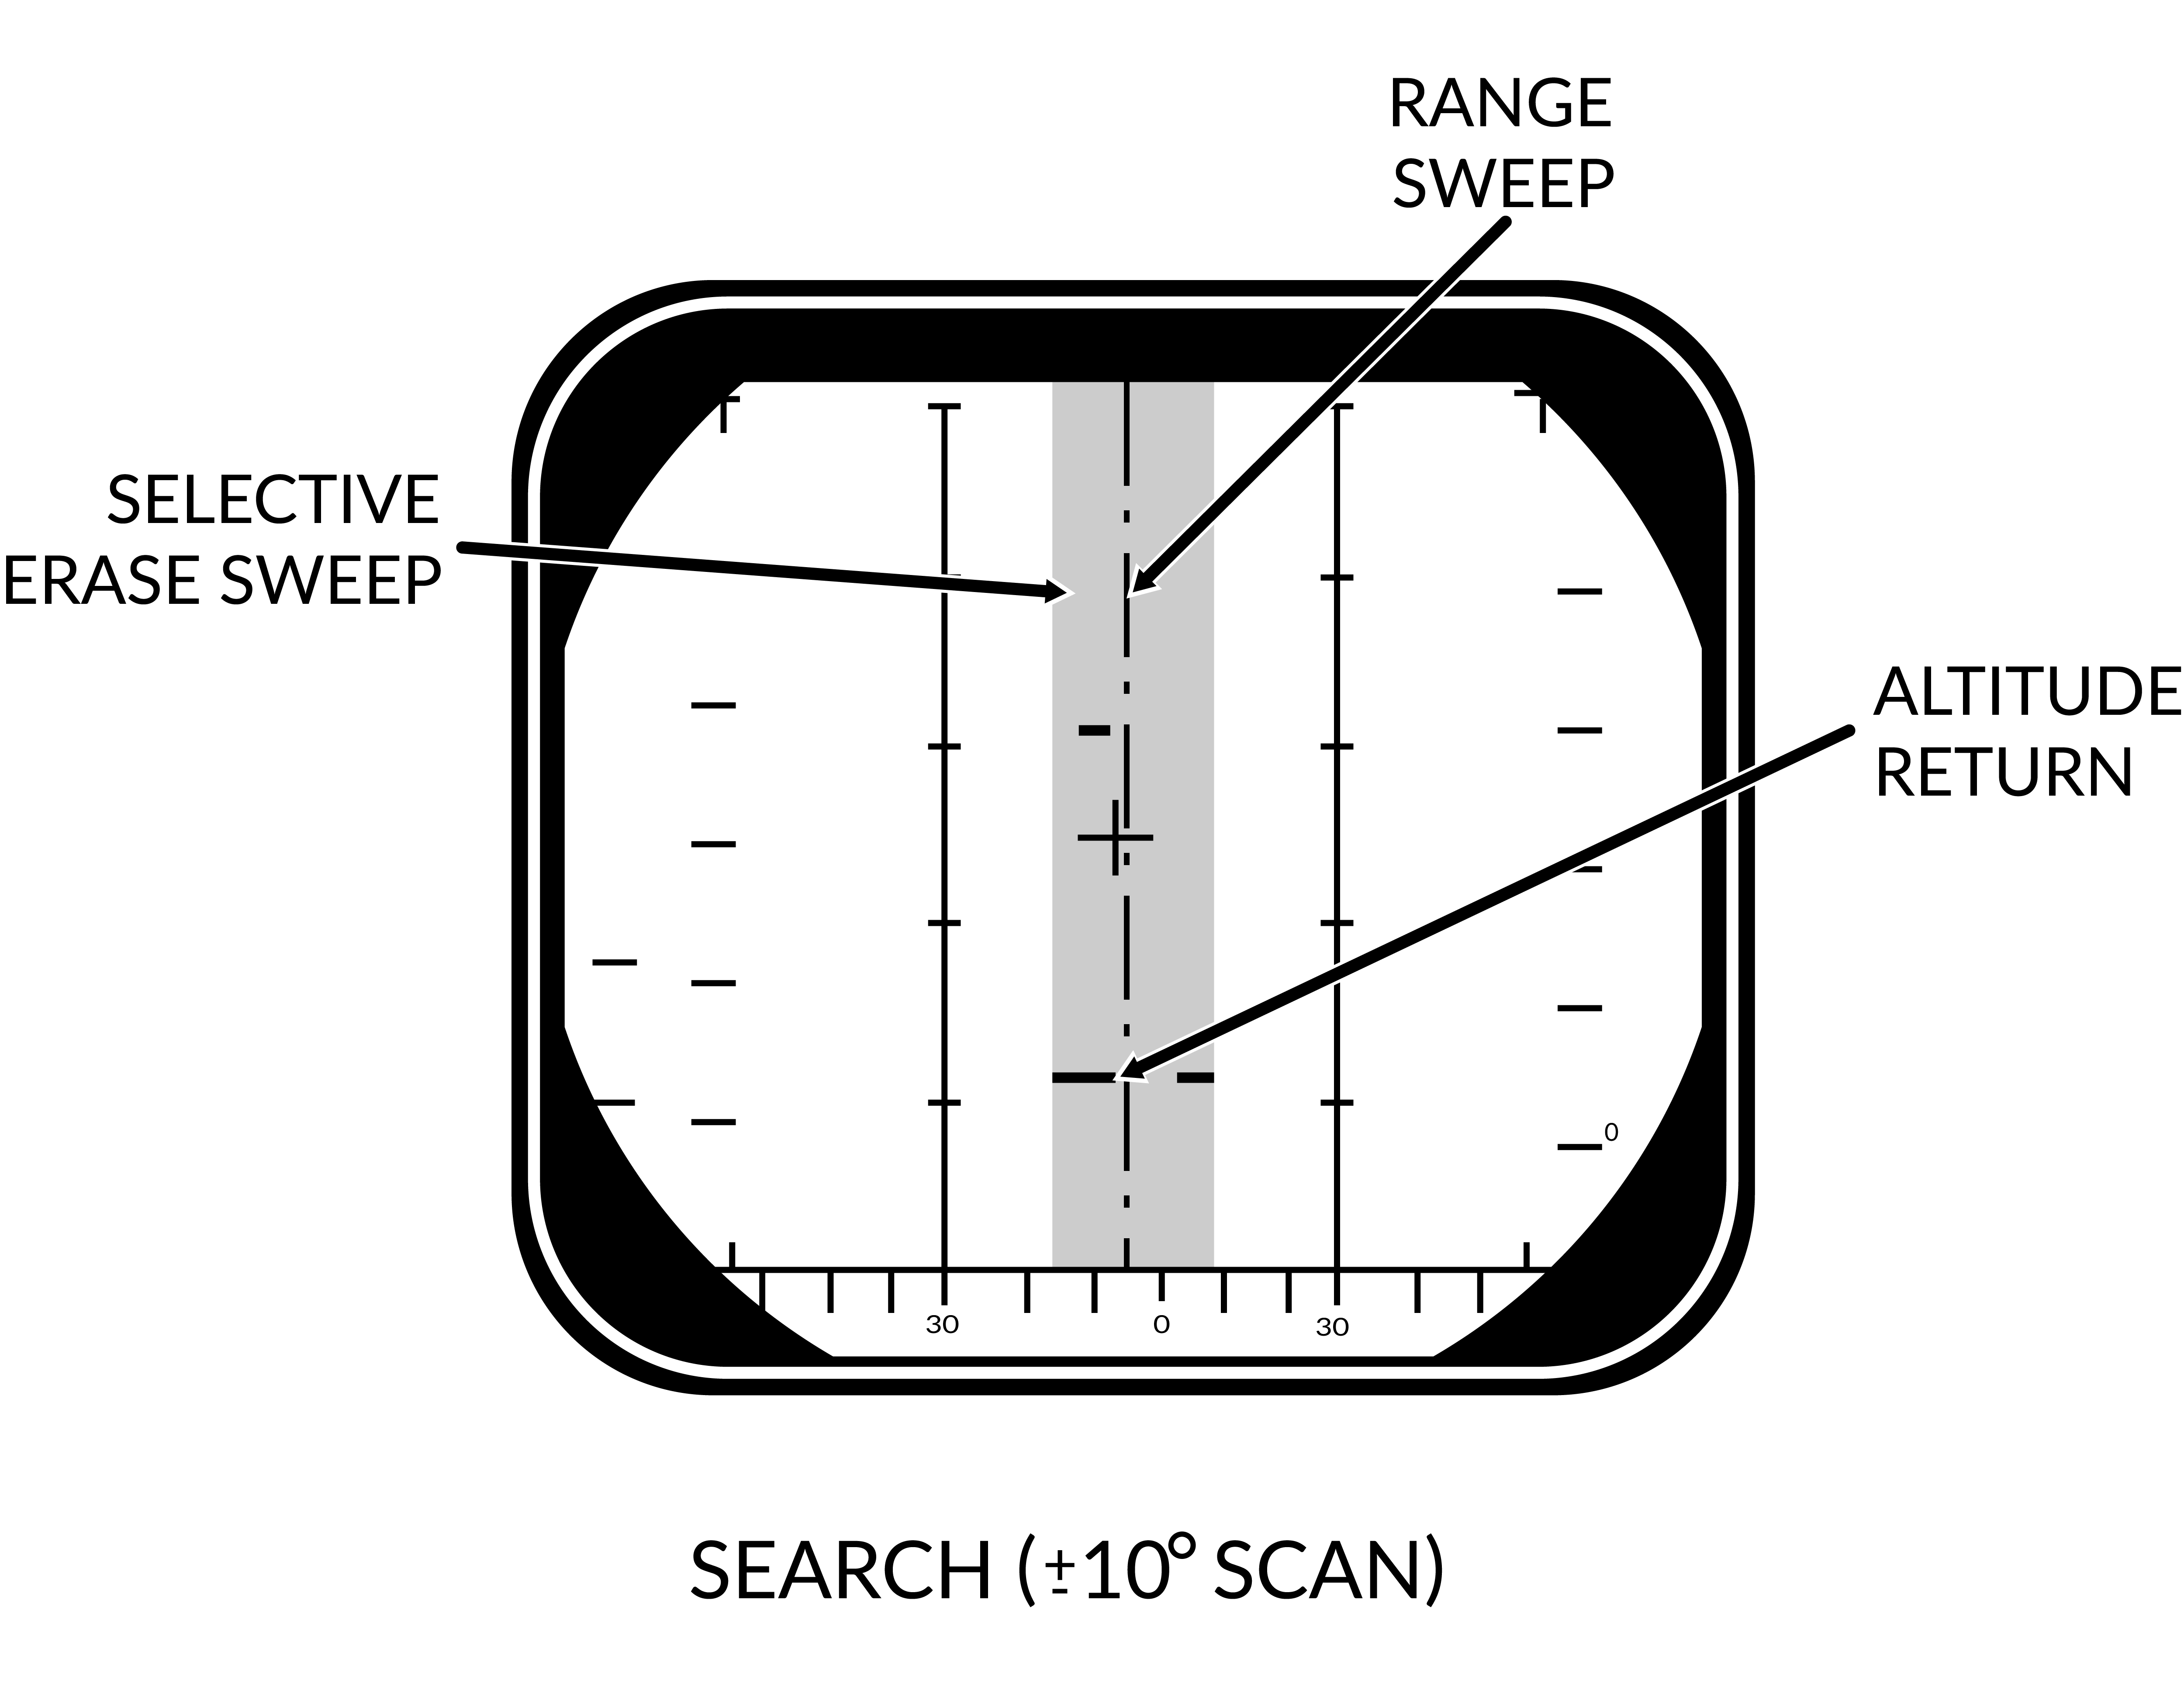
\includegraphics[width=0.8\linewidth]{PSEARCH.png}
		\caption{\textbf{DDD Format in Pulse Search Mode}}
		\label{fig:psearch}
	\end{figure}
	\begin{tableitemize}
		\blueitem{Pulse Search}{\textbf{Basic Mode} - AWG-9 does not use pulse doppler filtering

		\begin{subitemize}
			\item \textbf{Advantages}
			\begin{itemize}
				\item All aspect target detection
				\item Cannot be notched
				\item Rudimentary ground mapping
			\end{itemize}
			\item \textbf{Disadvantages}
			\begin{itemize}
    			\item No ground return filtering 
				\item Lower range
			\end{itemize}
		\end{subitemize}}
		\blueitem{DDD}{
		\begin{subitemize}
			\item \textbf{Range/Azimuth}
			\item Visualization of radar and erase sweeps
		\end{subitemize}}
		\blueitem{TID}{
		\begin{subitemize}
			\item \textbf{No Information from Pulse}
			\item \textbf{Cannot guide AIM-54}
		\end{subitemize}}
	\end{tableitemize}


	\clearpage

	\subsection{PSTT}
	\begin{figure}[htbp]
		\centering
		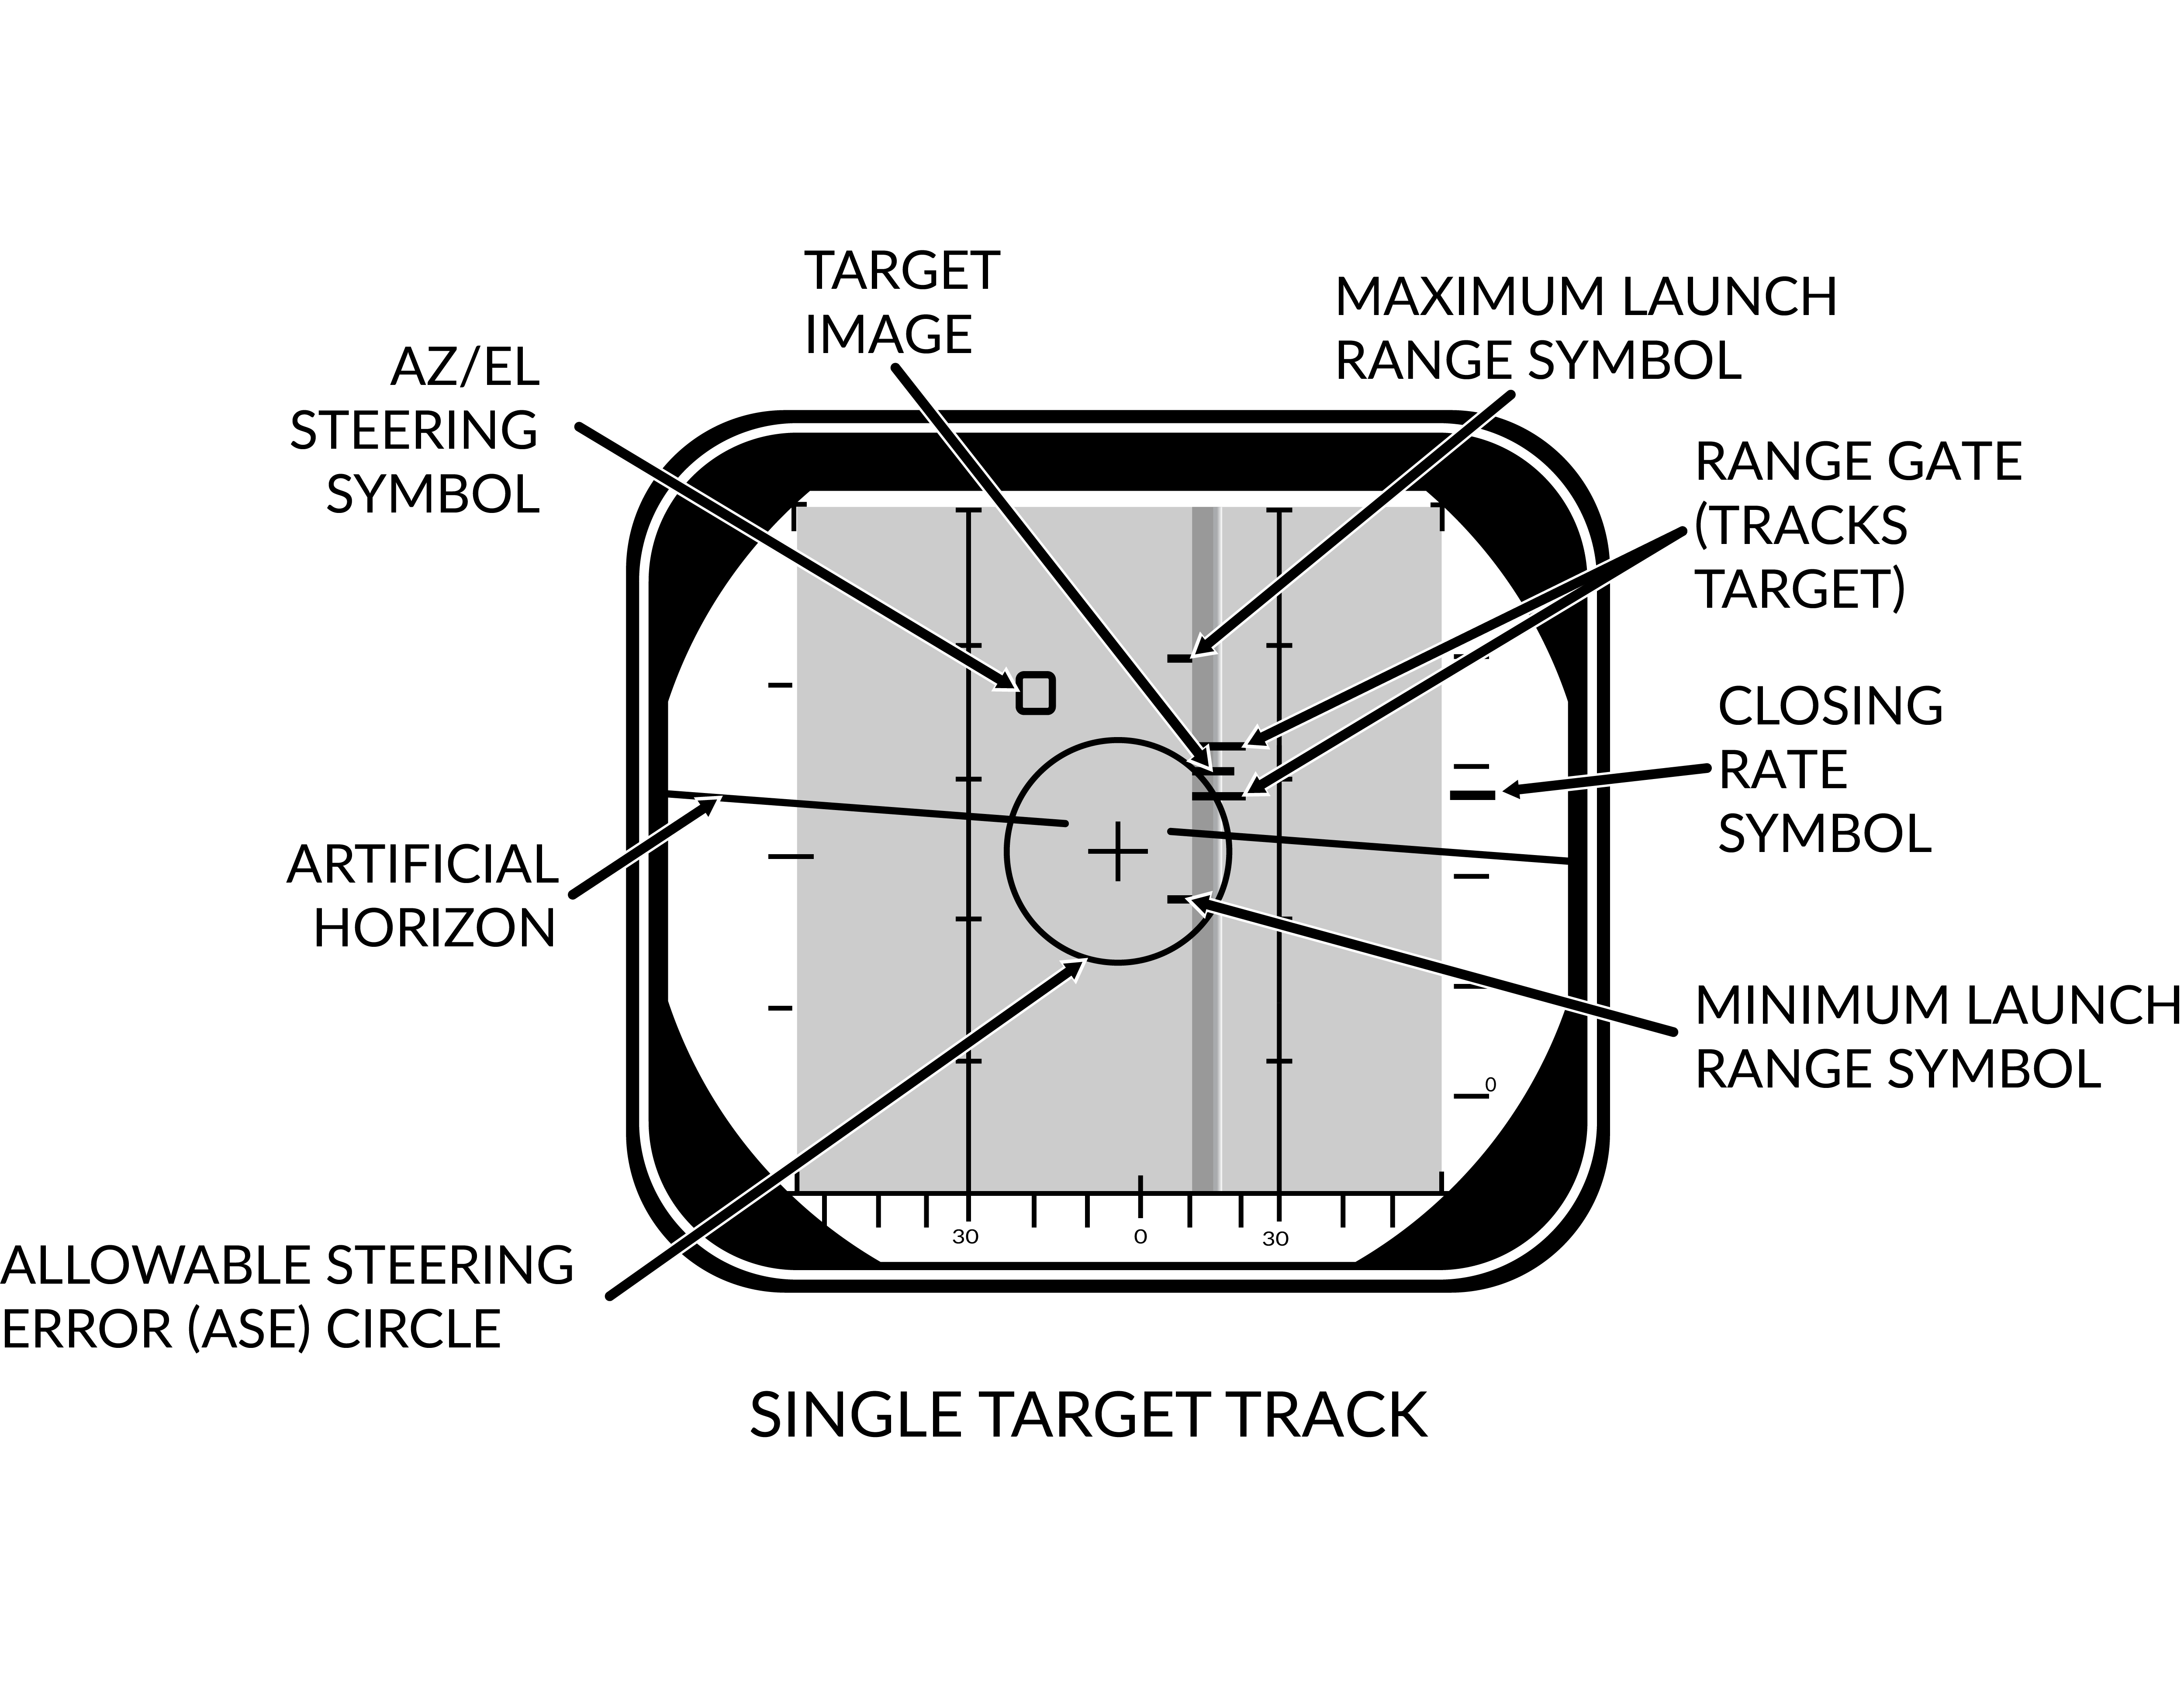
\includegraphics[width=0.90\linewidth]{PSTT.png}
		\caption{\textbf{DDD Format in PSTT Mode}}
		\label{fig:pstt}
	\end{figure}
	\begin{tableitemize}
		\blueitem{Pulse STT}{Lock Target w/o doppler filtering 
		\begin{subitemize}
			\item \textbf{Advantages} -- Cannot be notched
			\item \textbf{Disadvantages} -- Susceptible to ground clutter
		\end{subitemize}}
		\blueitem{DDD}{
		\begin{subitemize}
			\item \textbf{Track Indications}
			\begin{itemize}
				\item ANT TRK \& RDROT lights
				\item Tracking gates
				\item Closure rate
				\item Attack Symbology
			\end{itemize}
		\end{subitemize}}
	\end{tableitemize}

	\notebox{
		\begin{itemize}
			\item \textbf{PSTT Lock Affects Missile Logic}
			\begin{itemize}
				\item AIM-54 launched in \textbf{Active Launch Mode}
				\item AIM-7 launched in \textbf{CW Mode}
			\end{itemize}
		\end{itemize}
	}

	\clearpage

	\subsection{PSTT ACQUISITION}
	\begin{tableitemize}
		\blueitem{Pulse To PSTT}{
		\begin{subitemize}
			\item \textbf{Conditions}
			\begin{itemize}
				\item Pulse Search Mode selected
				\item RDR HCU Mode selected
			\end{itemize}
			\item \textbf{Lock Target}
			\begin{enumerate}
				\item Hold HCU Half-action
				\item Slew acquisition gates over desired Target on DDD
				\item HCU Full-Action to lock
			\end{enumerate}
			\item \textbf{Unlock Target}
			\begin{enumerate}[resume]
				\item HCU Half-action
			\end{enumerate}
		\end{subitemize}}
		\blueitem{TWS to PSTT}{
		\begin{subitemize}
			\item \textbf{Conditions}
			\begin{itemize}
				\item TWS Mode selected
				\item RDR HCU Mode selected
			\end{itemize}
			\item \textbf{Lock Target}
			\begin{enumerate}
				\item Hook Target on TID
				\item Press PSTT button on DDD Panel
			\end{enumerate}
			\item \textbf{Unlock Target}
			\begin{enumerate}[resume]
				\item HCU Half-action
			\end{enumerate}
		\end{subitemize}}
		\blueitem{ACM to PSTT}{
		\begin{subitemize}
			\item \textbf{Lock Target}
			\begin{enumerate}
				\item Select desired ACM Mode (Pilot or RIO)
				\item Place target in search volume through maneuvering
			\end{enumerate}
			\item \textbf{Unlock Target}
			\begin{enumerate}[resume]
				\item HCU Half-action
			\end{enumerate}
		\end{subitemize}}
		\blueitem{PDSTT to PSTT}{
		\begin{subitemize}
			\item \textbf{Conditions}
			\begin{itemize}
				\item Target PDSTT Locked
			\end{itemize}
			\item \textbf{Lock Target}
			\begin{enumerate}
				\item Press PSTT button on DDD Panel
			\end{enumerate}
			\item \textbf{Unlock Target}
			\begin{enumerate}[resume]
				\item HCU Half-action
			\end{enumerate}
		\end{subitemize}}
	\end{tableitemize}

	\clearpage

	\section{PULSE DOPPLER MODES}
	\subsection{PULSE DOPPLER SEARCH}
	\begin{figure}[htbp]
		\centering
		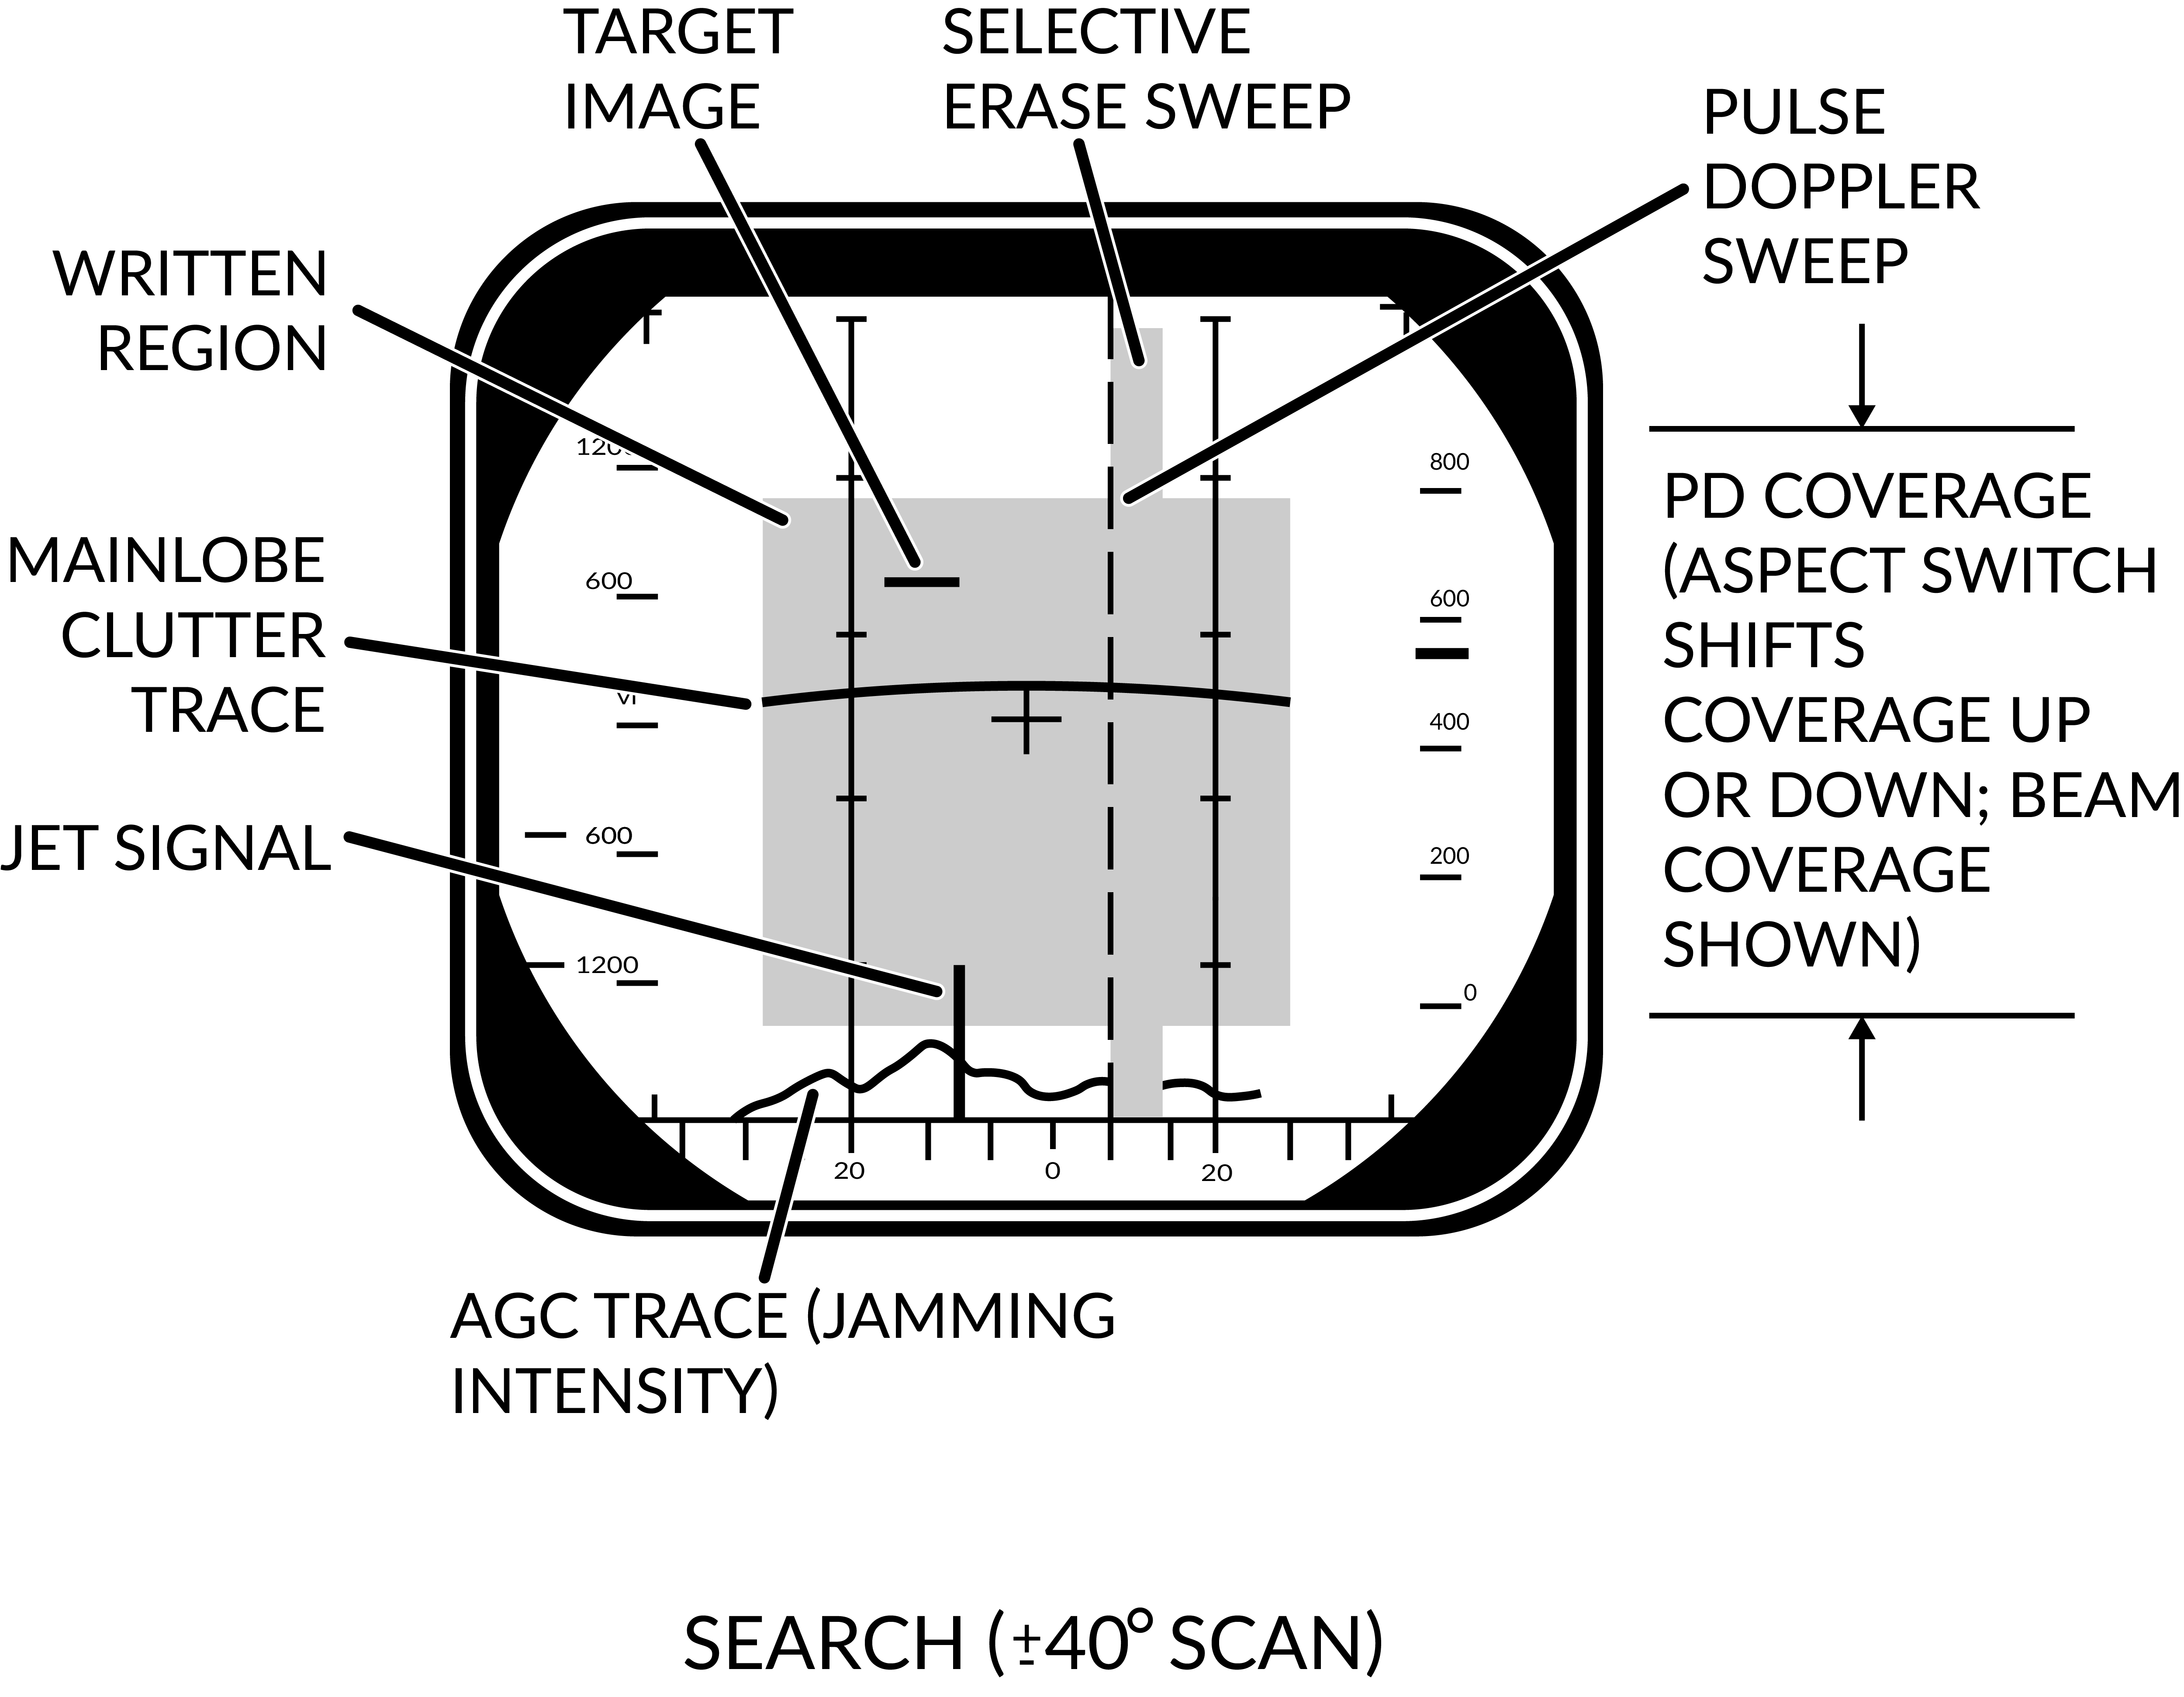
\includegraphics[width=0.9\linewidth]{PDSEARCH.png}
		\caption{\textbf{DDD Format in PD Search Mode}}
		\label{fig:pdsearch}
	\end{figure}
	\begin{tableitemize}
		\blueitem{Pulse Doppler Search}{ \textbf{``Early Warning'' Mode} - Longest Range, cannot display range

		\begin{subitemize}
			\item \textbf{Advantages}
			\begin{itemize}
				\item Longest Range
				\item Doppler Filtering
				\item \textbf{``Look Down Shoot Down''}
			\end{itemize}
			\item \textbf{Disadvantages}
			\begin{itemize}
				\item Can be notched
				\item No range information
			\end{itemize}
		\end{subitemize}}
		\blueitem{DDD}{
		\begin{subitemize}
			\item \textbf{Closure Rate/Azimuth}
			\item Visualization of radar and erase sweeps
		\end{subitemize}}
		\blueitem{Doppler Filters}{
		\begin{subitemize}
			\item \textbf{MLC -- Main Lobe Clutter Filter}
			\begin{itemize}
				\item \textbf{Own GS +/- 133 knots}
				\item Removes main ground return
				\item Source of notching
			\end{itemize}
			\item \textbf{ZD -- Zero Doppler Filter}
			\begin{itemize}
				\item \textbf{Negative own GS +/- 100 knots}
				\item Removes Radar reflection from ground directly beneath own AC
			\end{itemize}
		\end{subitemize}}
		\dblueitem{MLC Switch}{
		\begin{subitemize}
			\item \textbf{IN:} Enables MLC filter
			\item \textbf{AUTO:} Enables MLC filter if look-up angle less than 3 deg
			\item \textbf{OUT:} Disables MLC filter
		\end{subitemize}}
		\dblueitem{Vc Switch}{Changes closure rate DDD scale
		\begin{subitemize}
			\item \textbf{X-4:} -800 to 4000 knots
			\item \textbf{NORM:} -200 to 1000 knots
			\item \textbf{VID:} -50 to 250 knots
		\end{subitemize}}
		\blueitem{ASPECT Switch}{Changes closure rate processing scale
		\begin{subitemize}
			\item \textbf{NOSE:} -600 to 1800 knots
			\item \textbf{BEAM:} -1200 to 1200 knots
			\item \textbf{TAIL:} -1800 to 600 knots
		\end{subitemize}}
	\end{tableitemize}

	\clearpage

	\begin{figure}[htbp]
		\centering
		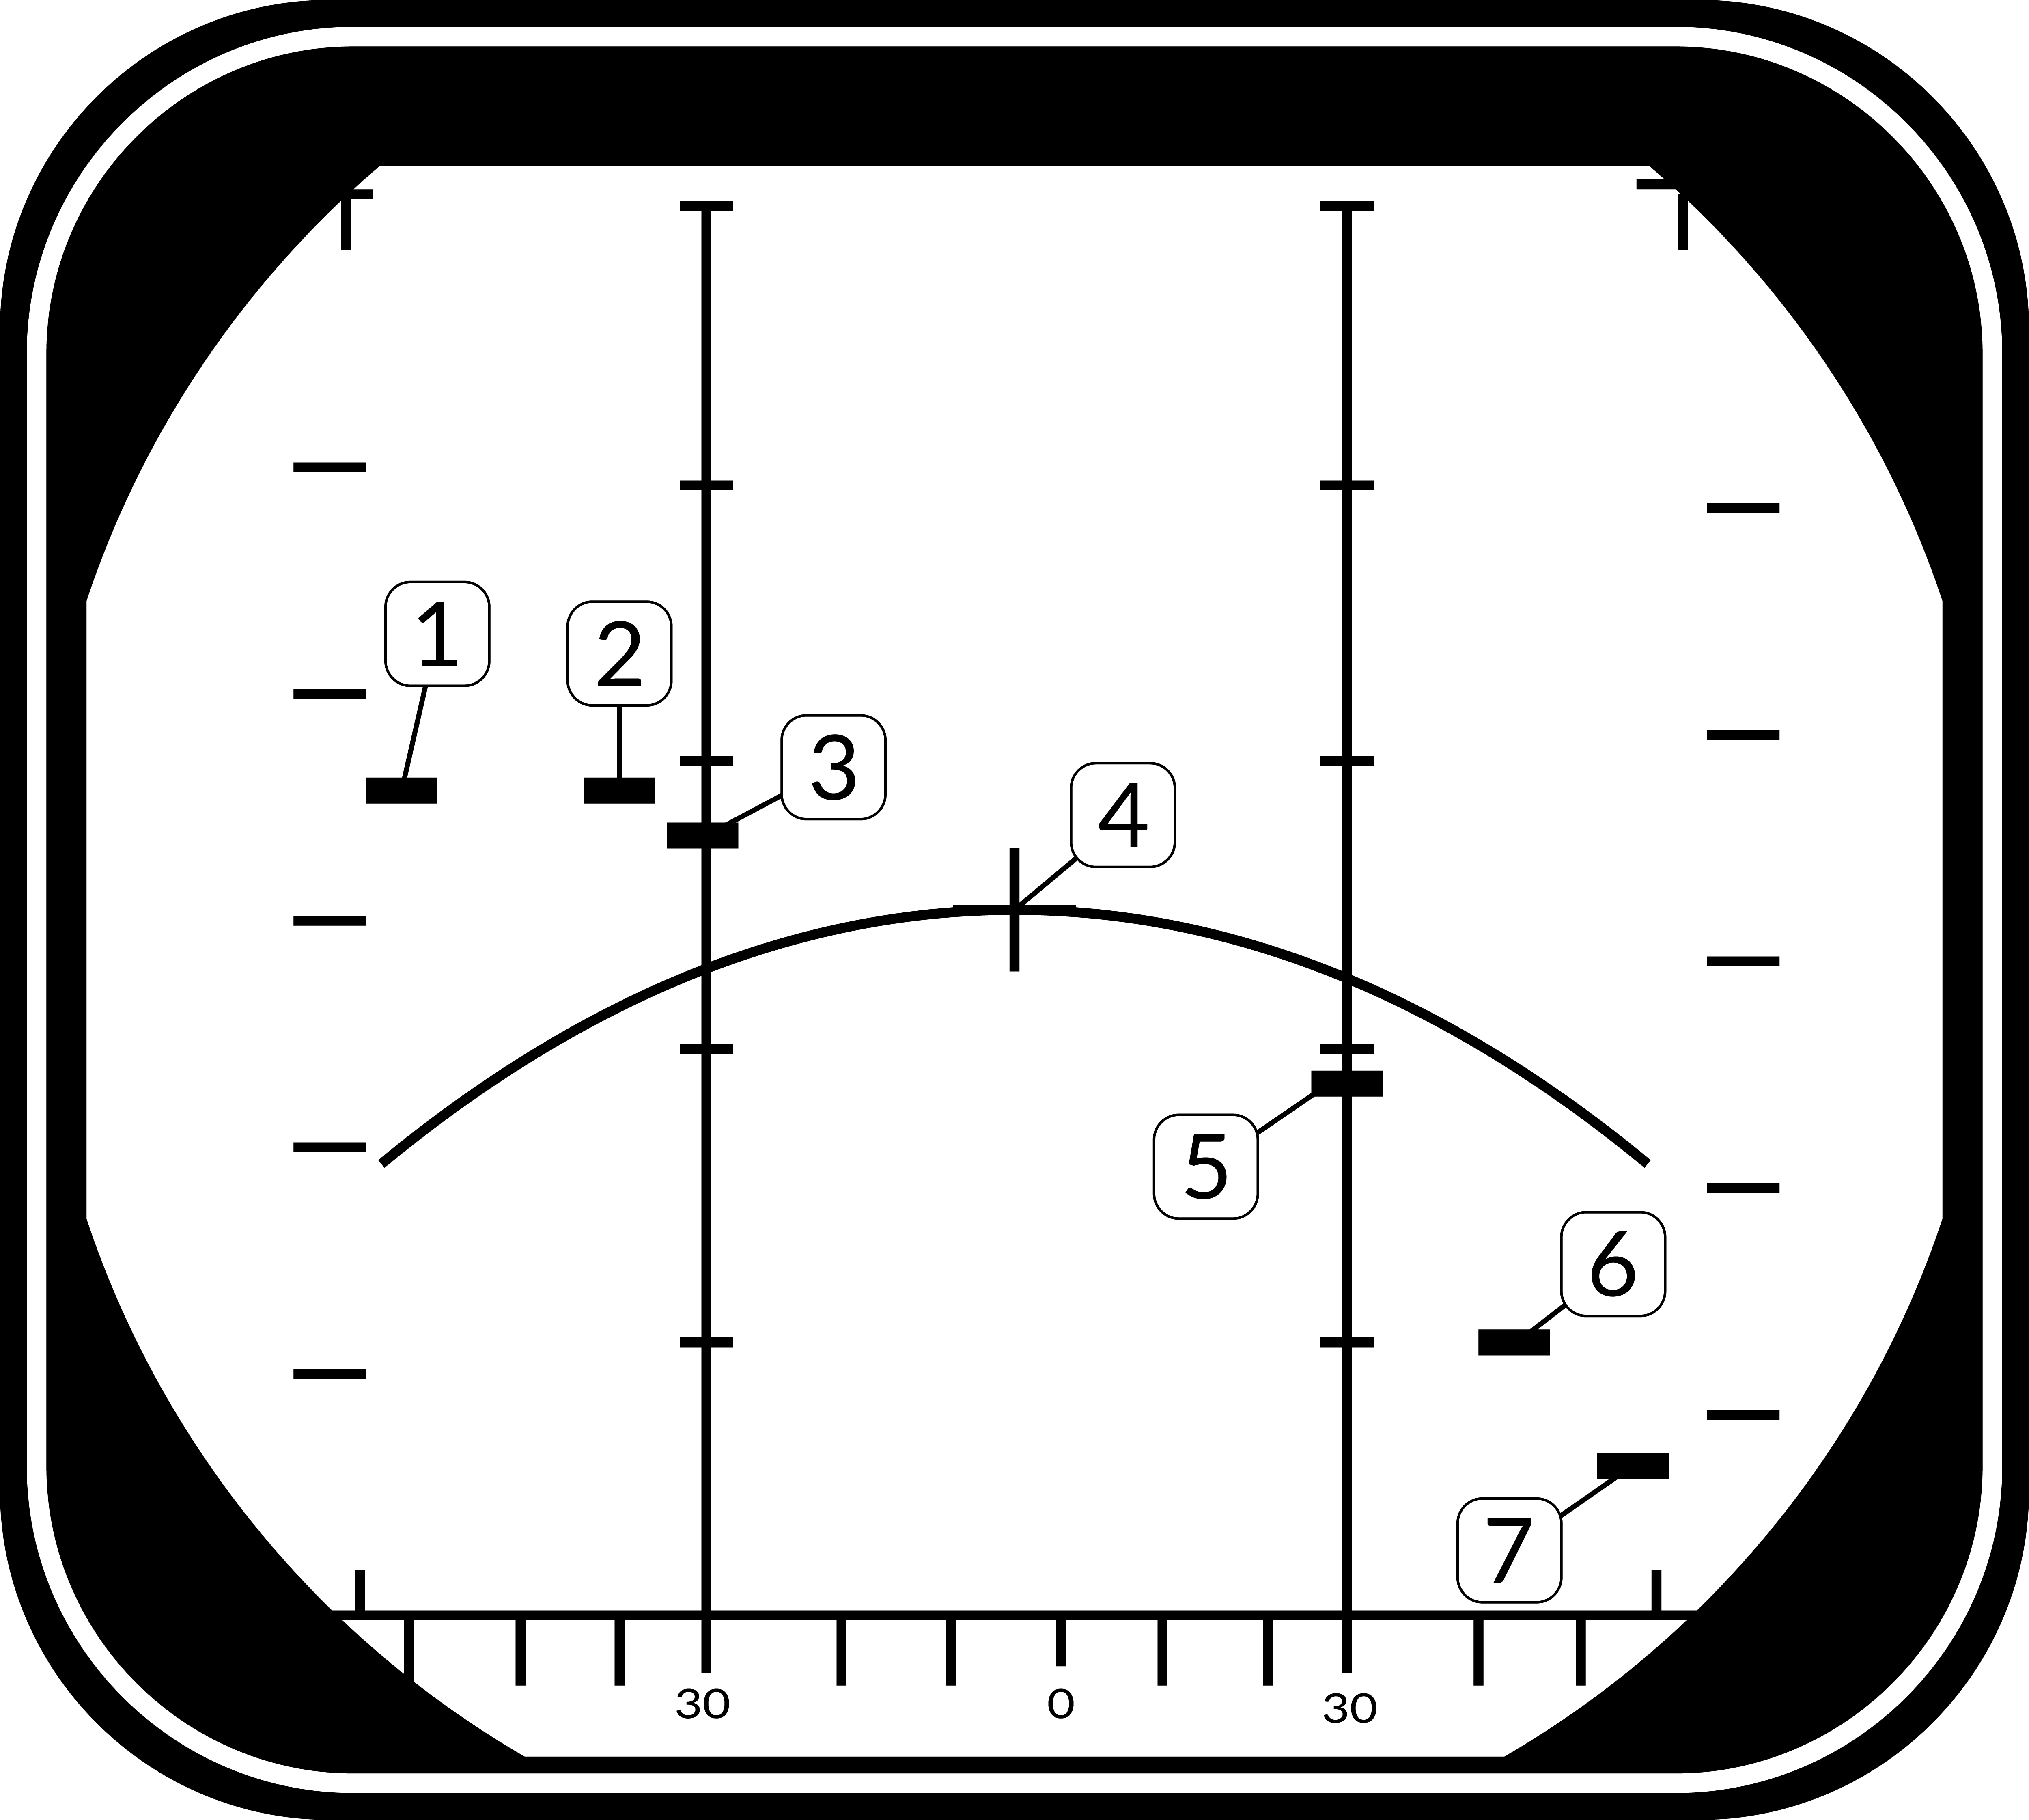
\includegraphics[width=0.5\linewidth]{PD.png}
		\caption{\textbf{DDD Showing Contacts in PD Mode}}
		\label{fig:pd}
	\end{figure}
	\begin{table}[htbp]
		\centering 
		\caption{\textbf{Target Data for \Cref{fig:pd}}}
		\label{tab:pddata}
		\begin{longtable}{l | l | l | l}
			\toprule
			& \blue{Look Angle} & \blue{Line of Sight Rate} & \blue{Target Heading} \\
			\midrule
			\textbf{1} & 60 deg & 1490 & 180 deg \\
			\midrule
			\textbf{2} & 45 deg & 1500 & 120 deg \\
			\midrule
			\textbf{3} & 30 deg & 1428 & 100 deg \\
			\midrule
			\textbf{4} & 0 deg & 1200 & 90 deg \\
			\midrule
			\textbf{5} & 30 deg & 672 & 80 deg \\
			\midrule
			\textbf{6} & 45 deg & 210 & 60 deg \\
			\midrule
			\textbf{7} & 60 deg & -300 & 0 deg \\
			\bottomrule
		\end{longtable}
	\end{table}

	\notebox{
		\begin{itemize}
			\item Target \textbf{4} is \emph{notching} and thus shows no radar return
		\end{itemize}
	}
	
	\clearpage


	\subsection{RWS}
	\label{sec:awg9-rws}
	\begin{tableitemize}
		\blueitem{Range While Search}{\textbf{FM Ranging}, used for getting good A/A picture before selecting TWS

		\begin{subitemize}
			\item \textbf{FM Ranging}
			\begin{itemize}
				\item Pulse Doppler with ranging
				\item TID shows momentary tracks with ranges
				\item Processing reduces max range
			\end{itemize}
			\item \textbf{Advantages}
			\begin{itemize}
				\item Long Range
				\item Doppler Filtering
				\item \textbf{``Look Down Shoot Down''}
				\item Signal Processing
			\end{itemize}
			\item \textbf{Disadvantages}
			\begin{itemize}
				\item Can be notched
			\end{itemize}
		\end{subitemize}}
		\blueitem{DDD}{
		\begin{subitemize}
			\item \textbf{Closure Rate/Azimuth}
			\item Visualization of radar and erase sweeps
		\end{subitemize}}
		\blueitem{TID}{
		\begin{subitemize}
			\item \textbf{Momentary Tracks}
			\item Max concurrent tracks: 48
			\item \textbf{Cannot lock targets from TID}
		\end{subitemize}}
		\blueitem{Doppler Filters}{
		\begin{subitemize}
			\item \textbf{MLC -- Main Lobe Clutter Filter}
			\begin{itemize}
				\item \textbf{Own GS +/- 133 knots}
				\item Removes main ground return
				\item Source of notching
			\end{itemize}
			\item \textbf{ZD -- Zero Doppler Filter}
			\begin{itemize}
				\item \textbf{Negative own GS +/- 100 knots}
				\item Removes Radar reflection from ground directly beneath own AC
			\end{itemize}
		\end{subitemize}}
	\end{tableitemize}

	\clearpage

	\subsection{TWS}
	\label{sec:awg9-tws}
	
	\begin{tableitemize}
		\blueitem{Track While Scan}{\textbf{Builds Track Files}, high situational awareness, multi-target AIM-54 launch
		
		\begin{subitemize}
			\item \textbf{Track Files}
			\begin{itemize}
				\item AWG-9 builds Trackfiles for contacts
				\item Can launch multiple AIM-54
				\item Processing reduces max range
				\item Can lock targets from TID
			\end{itemize}
			\item \textbf{FM Ranging}
			\begin{itemize}
				\item Pulse Doppler with ranging
				\item TID shows momentary tracks with ranges
				\item Processing reduces max range
			\end{itemize}
			\item \textbf{Advantages}
			\begin{itemize}
				\item Doppler Filtering
				\item \textbf{Multi-Target AIM-54}
			\end{itemize}
			\item \textbf{Disadvantages}
			\begin{itemize}
				\item \textbf{Lowest Range}
				\item Can be notched
			\end{itemize}
		\end{subitemize}}
		\blueitem{DDD}{
		\begin{subitemize}
			\item \textbf{Closure Rate/Azimuth}
			\item Visualization of radar and erase sweeps
		\end{subitemize}}
		\blueitem{TID}{
		\begin{subitemize}
			\item \textbf{Tracksfiles}
			\item Max concurrent tracks: 24
			\item Max displayed tracks: 18
		\end{subitemize}}
		\blueitem{Doppler Filters}{
		\begin{subitemize}
			\item \textbf{MLC -- Main Lobe Clutter Filter}
			\begin{itemize}
				\item \textbf{Own GS +/- 133 knots}
				\item Removes main ground return
				\item Source of notching
			\end{itemize}
			\item \textbf{ZD -- Zero Doppler Filter}
			\begin{itemize}
				\item \textbf{Negative own GS +/- 100 knots}
				\item Removes Radar reflection from ground directly beneath own AC
			\end{itemize}
		\end{subitemize}}
		\blueitem{Scan Volume}{Trackfiles require update every 2.5 s -->
		\begin{subitemize}
			\item 20 deg 4 bar (if selected)
			\item 40 deg 2 bar (else)
		\end{subitemize}}
		\blueitem{TID Mode \break Selector}{
		\begin{subitemize}
			\item \textbf{GND STAB:} Ground Stabilized, True North is up on TID
			\item \textbf{A/C STAB:} Aircraft Stabilized
			\item \textbf{ATTAK:} same as A/C STAB with superimposed attack steering symbology
			\item \textbf{TV:} Displays TCS on TID, dispays LANTIRN on TID if equipped
		\end{subitemize}}
		\blueitem{TID Display Selector \break Buttons}{
		\begin{subitemize}
			\item \textbf{RID DISABLE:} Not simulated
			\item \textbf{ALT NUM:} Enables display of track altitudes on left side of track symbols
			\item \textbf{SYM ELEM:} Enables display of all supplementary symbology of tracks and waypoints
			\item \textbf{DATA LINK:} Enables display of D/L contacts
			\item \textbf{JAM STROBE:} Enables display of jam strobes
			\item \textbf{NON-ATTK:} enables/disables display of targets not possible to engage (friendlies)
			\item \textbf{LAUNCH ZONE:} Enables display of weapon launch zones
			\item \textbf{VEL VECTOR:} Enables display of velocity vectors
		\end{subitemize}}
		\blueitem{TRACK HOLD \break CLSN Steering \break Buttons}{
		\begin{subitemize}
			\item \textbf{TRACK HOLD}
			\begin{itemize}
				\item Normally: Tracks maintained for 14 s after last observation
				\item Track Hold: maintained for 2 min after last observation
			\end{itemize}
			\item \textbf{CLSN Button}
			\begin{itemize}
				\item begins collision steering to currently tracked target
				\item enables Steering Centroid if in TWS
				\item LD CLSN presents azimuth steering only
				\item CLSN presents both azimuth and elevation steering
			\end{itemize}
		\end{subitemize}}
		\blueitem{TWS AUTO / MAN}{
		\begin{subitemize}
			\item \textbf{TWS MAN:} Manual azimuth/elevation control, target designation by RIO
			\item \textbf{TWS AUTO:} Automatic prioritization of targets and azimuth elevation control
		\end{subitemize}}
	\end{tableitemize}

	\clearpage

	\subsection{TWS MAN}
	\begin{tableitemize}
		\blueitem{TWS MAN}{
		\begin{subitemize}
			\item \textbf{Target Selection:} Manual
			\item \textbf{Scan Azimuth/Elevation:} Manual
		\end{subitemize}}
		\blueitem{Target Selection}{
		\begin{subitemize}
			\item \textbf{Conditions}
			\begin{itemize}
				\item TWS MAN Radar Mode selected
				\item TID CURSOR TID Mode selected
			\end{itemize}
			\item \textbf{Hook Target}
			\begin{enumerate}
				\item Hold HCU Half-Action
				\item Slew TID Cursor over desired Tgt
				\item HCU Full-Action to select Tgt
			\end{enumerate}
			\item \textbf{TID Symbology}
			\begin{itemize}
				\item Range (\textbf{RA})
				\item Bearing (\textbf{BR})
				\item Altitude (\textbf{AL})
				\item Magnetic course (\textbf{MC})
			\end{itemize}
			\item \textbf{Lock Target}
			\begin{enumerate}[label=(\alph*), resume]
				\item Press \textbf{PD STT} or \textbf{Pulse STT} buttons
			\end{enumerate}
			\item \textbf{Deselect Target}
			\begin{enumerate}[label=(\alph*), resume]
				\item press HCU Half-Action
			\end{enumerate}
		\end{subitemize}}
		\blueitem{AIM-54 Launch}{
		\begin{subitemize}
			\item \textbf{Automatically selects TWS AUTO}
			\item \textbf{Prevents selection of TWS MAN}
		\end{subitemize}}
	\end{tableitemize}

	\clearpage

	\subsection{TWS AUTO}
	\begin{tableitemize}
		\blueitem{TWS AUTO}{
		\begin{subitemize}
			\item \textbf{Target Selection:} prioritizes contacts based off range, aspect, closure
			\item \textbf{Scan Azimuth/Elevation:} Geometric center of targets in scan volume
		\end{subitemize}}
		\blueitem{Centroid / Steering Cues}{
		\begin{subitemize}
			\item \textbf{Steering Centroid}
			\begin{itemize}
				\item facilitates steering cues
				\item HUD, VDI, TID, DDD
				\item Appears as \textbf{X} on TID
				\item Takes Gimbal limits into account
				\item Weights individual Tracks based on parameters
			\end{itemize}
			\item \textbf{Illumination Centroid}
			\begin{itemize}
				\item \textbf{Not Visible}
				\item Controls azimuth and elevation of scan pattern
				\item Takes scan volume into account
			\end{itemize}
		\end{subitemize}}
		\blueitem{Pilot Steering Cues}{
		\begin{subitemize}
			\item \textbf{Conditions}
			\begin{itemize}
				\item A-A HUD Mode selected
				\item Master Arm ON (UP)
				\item AIM-54 or AIM-7 selected
				\item TWS-AUTO selected
			\end{itemize}
		\end{subitemize}}
	\end{tableitemize}

	\clearpage

	\subsection{PDSTT}
	\begin{figure}[htbp]
		\centering
		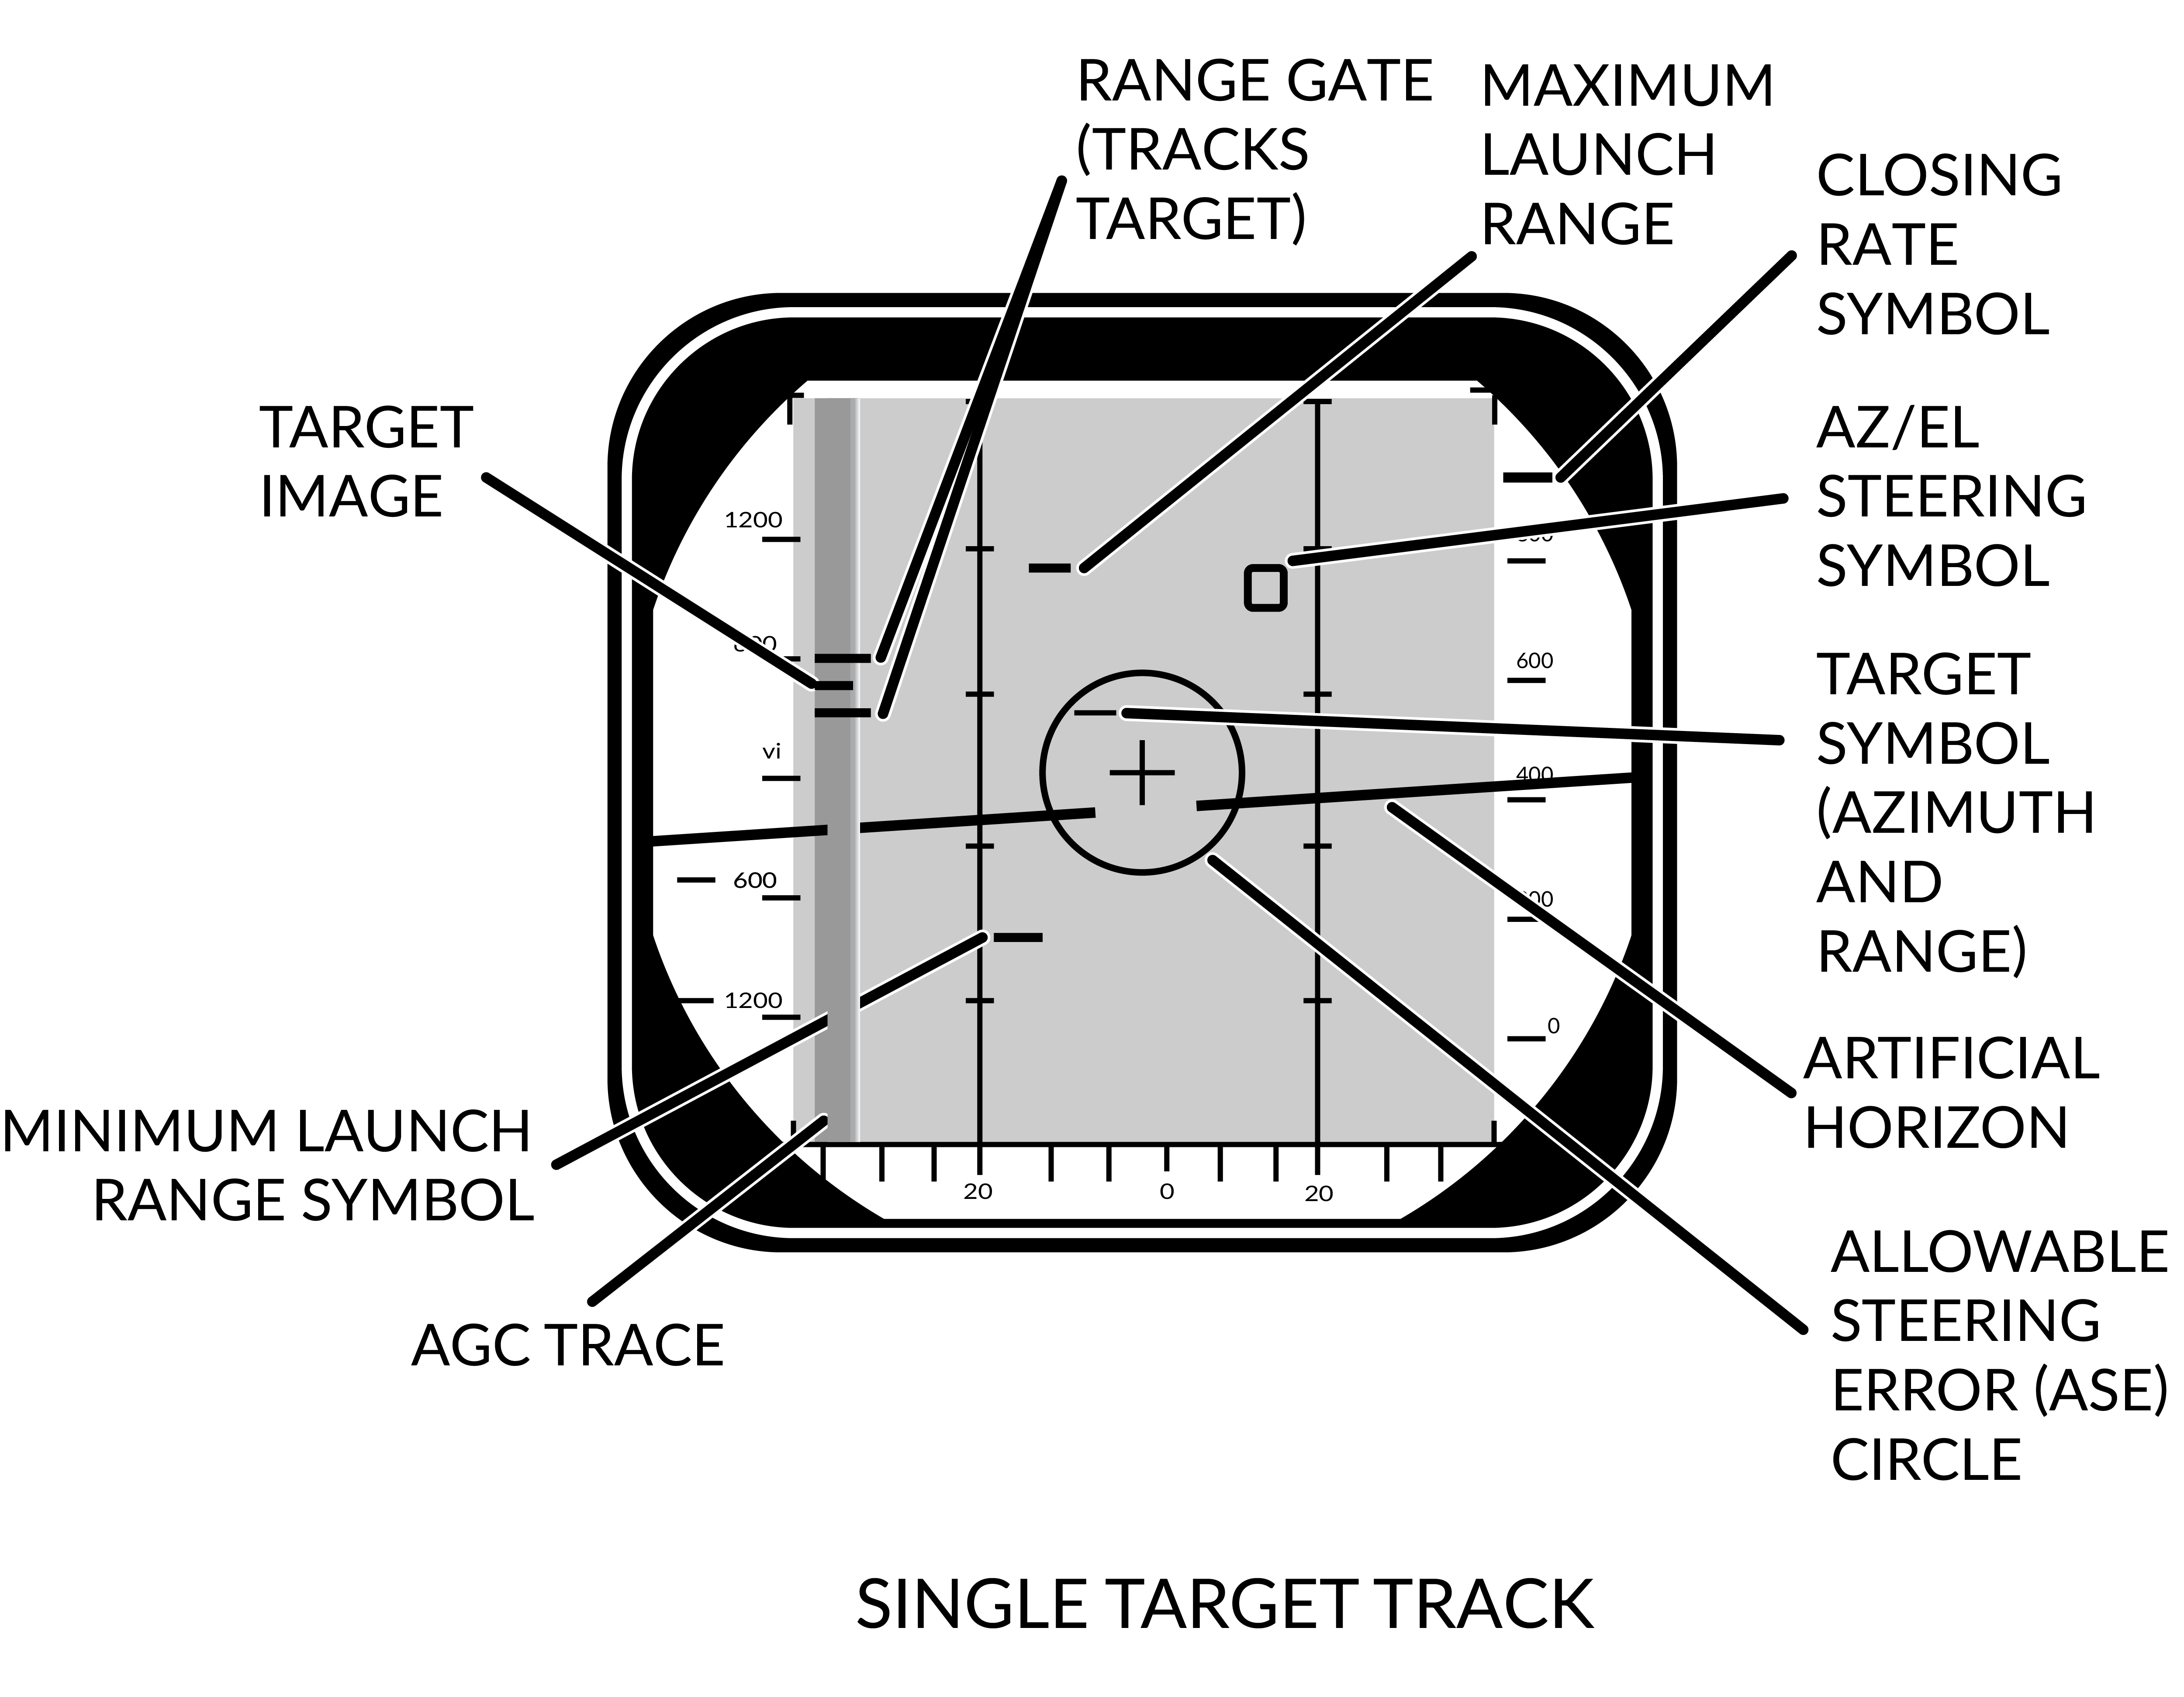
\includegraphics[width=0.9\linewidth]{PDSTT.png}
		\caption{\textbf{DDD Format in PDSTT Mode}}
		\label{fig:pdstt}
	\end{figure}
	\begin{tableitemize}
		\blueitem{Pulse Doppler STT}{
		\begin{subitemize}
			\item \textbf{Advantages} -- Ground Clutter filtering
			\item \textbf{Disadvantages} -- Susceptible to notching
		\end{subitemize}}
		\blueitem{DDD}{
		\begin{subitemize}
			\item \textbf{Track Indications}
			\begin{itemize}
				\item ANT TRK \& RDROT lights
				\item Tracking gates
				\item Closure rate
				\item Attack Symbology
			\end{itemize}
		\end{subitemize}}
	\end{tableitemize}

	\notebox{
		\begin{itemize}
			\item \textbf{PDSTT Lock Affects Missile Logic}
			\begin{itemize}
				\item Enables launch of AIM-54/AIM-7 in \textbf{PD Mode}
    			\item AIM-7 PD launch requires \textbf{MSL OPTIONS Switch} to be in \textbf{SP PD}  
			\end{itemize}
		\end{itemize}
	}

	\clearpage

	\subsection{PDSTT ACQUISITION}
	\begin{tableitemize}
		\blueitem{PD To PDSTT}{
		\begin{subitemize}
			\item \textbf{Conditions}
			\begin{itemize}
				\item PD Search Mode selected
				\item RDR HCU Mode selected
			\end{itemize}
			\item \textbf{Lock Target}
			\begin{enumerate}
				\item Hold HCU Half-action
				\item Slew acquisition gates over desired Target on DDD
				\item HCU Full-Action to lock
			\end{enumerate}
			\item \textbf{Unlock Target}
			\begin{enumerate}[resume]
				\item HCU Half-action
			\end{enumerate}
		\end{subitemize}}
		\blueitem{TWS to PDSTT}{
		\begin{subitemize}
			\item \textbf{Conditions}
			\begin{itemize}
				\item TWS Mode selected
				\item RDR HCU Mode selected
			\end{itemize}
			\item \textbf{Lock Target}
			\begin{enumerate}
				\item Hook Target on TID
				\item Press PDSTT button on DDD Panel
			\end{enumerate}
			\item \textbf{Unlock Target}
			\begin{enumerate}[resume]
				\item HCU Half-action
			\end{enumerate}
		\end{subitemize}}
		\blueitem{PSTT to PDSTT}{
		\begin{subitemize}
			\item \textbf{Conditions}
			\begin{itemize}
				\item Target PSTT Locked
			\end{itemize}
			\item \textbf{Lock Target}
			\begin{enumerate}
				\item Press PDSTT button on DDD Panel
			\end{enumerate}
			\item \textbf{Unlock Target}
			\begin{enumerate}[resume]
				\item HCU Half-action
			\end{enumerate}
		\end{subitemize}}
	\end{tableitemize}

	\clearpage

	\section{ACM MODES}
	\subsection{OVERVIEW}
	\begin{center}
		\begin{tabular}{p{3cm} | p{2cm}  | p{2cm} | p{2cm} | p{2cm}}
			\toprule
			& \blue{PLM} & \blue{VSL} & \blue{PAL} & \blue{MRL} \\
			\midrule
			\textbf{Range} & 5 nm & 5 nm & 15 nm & 5 nm \\
			\midrule
			\textbf{Description} & Boresight & Vertical & Horizontal & RIO \\
			\midrule
			\textbf{Weapons} & \multicolumn{4}{c}{Gun + All Missiles} \\
			\bottomrule
		\end{tabular}
	\end{center}

	\begin{tableitemize}
		\blueitem{PLM}{
		\begin{subitemize}
			\item \textbf{Pilot Lockon Mode} -- see \Cref{fig:acmvisplm}
			\item \textbf{Highest Priority ACM}
			\item \textbf{Search Pattern}
			\begin{itemize}
				\item Small Boresight
				\item Range: 5 nm
			\end{itemize}
		\end{subitemize}}
		\blueitem{VSL}{
		\begin{subitemize}
			\item \textbf{Vertical Scan Lockon} -- see \Cref{fig:acmvisvsl}
			\item \textbf{HI Search Pattern}
			\begin{itemize}
				\item Width: 5 deg
				\item Vertical: +15 to +55 deg
				\item Range: 5 nm
			\end{itemize}
			\item \textbf{LO Search Pattern}
			\begin{itemize}
				\item Width: 5 deg
				\item Vertical: -15 to +25 deg
				\item Range: 5 nm
			\end{itemize}
			\item \textbf{RIO/PILOT Controlled}
		\end{subitemize}}
		\blueitem{PAL}{
		\begin{subitemize}
			\item \textbf{Pilot Automatic Lockon}
			\item \textbf{Search Pattern}
			\begin{itemize}
				\item Width: +/- 20 deg
				\item Vertical: 8-bar
				\item Range: 15 nm
			\end{itemize}
		\end{subitemize}}
		\blueitem{MRL}{
		\begin{subitemize}
			\item \textbf{Manual Rapid Lockon} -- see \Cref{fig:acmvismrl}
			\item \textbf{RIO Controlled}
			\item \textbf{Search Pattern}
			\begin{itemize}
				\item HCU Controlled
				\item Range: 5 nm
			\end{itemize}
		\end{subitemize}}
	\end{tableitemize}

	\notebox{
		\begin{itemize}
			\item \textbf{ACM Modes Result in PSTT Lock} -- affects missile logic
			\begin{itemize}
				\item AIM-54 launched in \textbf{Active Launch Mode}
				\item AIM-7 launched in \textbf{CW Mode}
			\end{itemize}
		\end{itemize}
	}
	\warningbox{
		\begin{itemize}
			\item \textbf{Active Launch Mode Phoenixes Have Limited IFF Capability} 
			\begin{itemize}
				\item Employ with caution when friendlies airborne
			\end{itemize}
		\end{itemize}
	}

	\begin{figure}[htbp]
		\centering
		\begin{subfigure}[c]{0.55\linewidth}
			\centering
			\includegraphics[width=0.8\linewidth]{PLM.png}
			\subcaption{\textbf{PLM Search Pattern}}
			\label{fig:acmvisplm}
			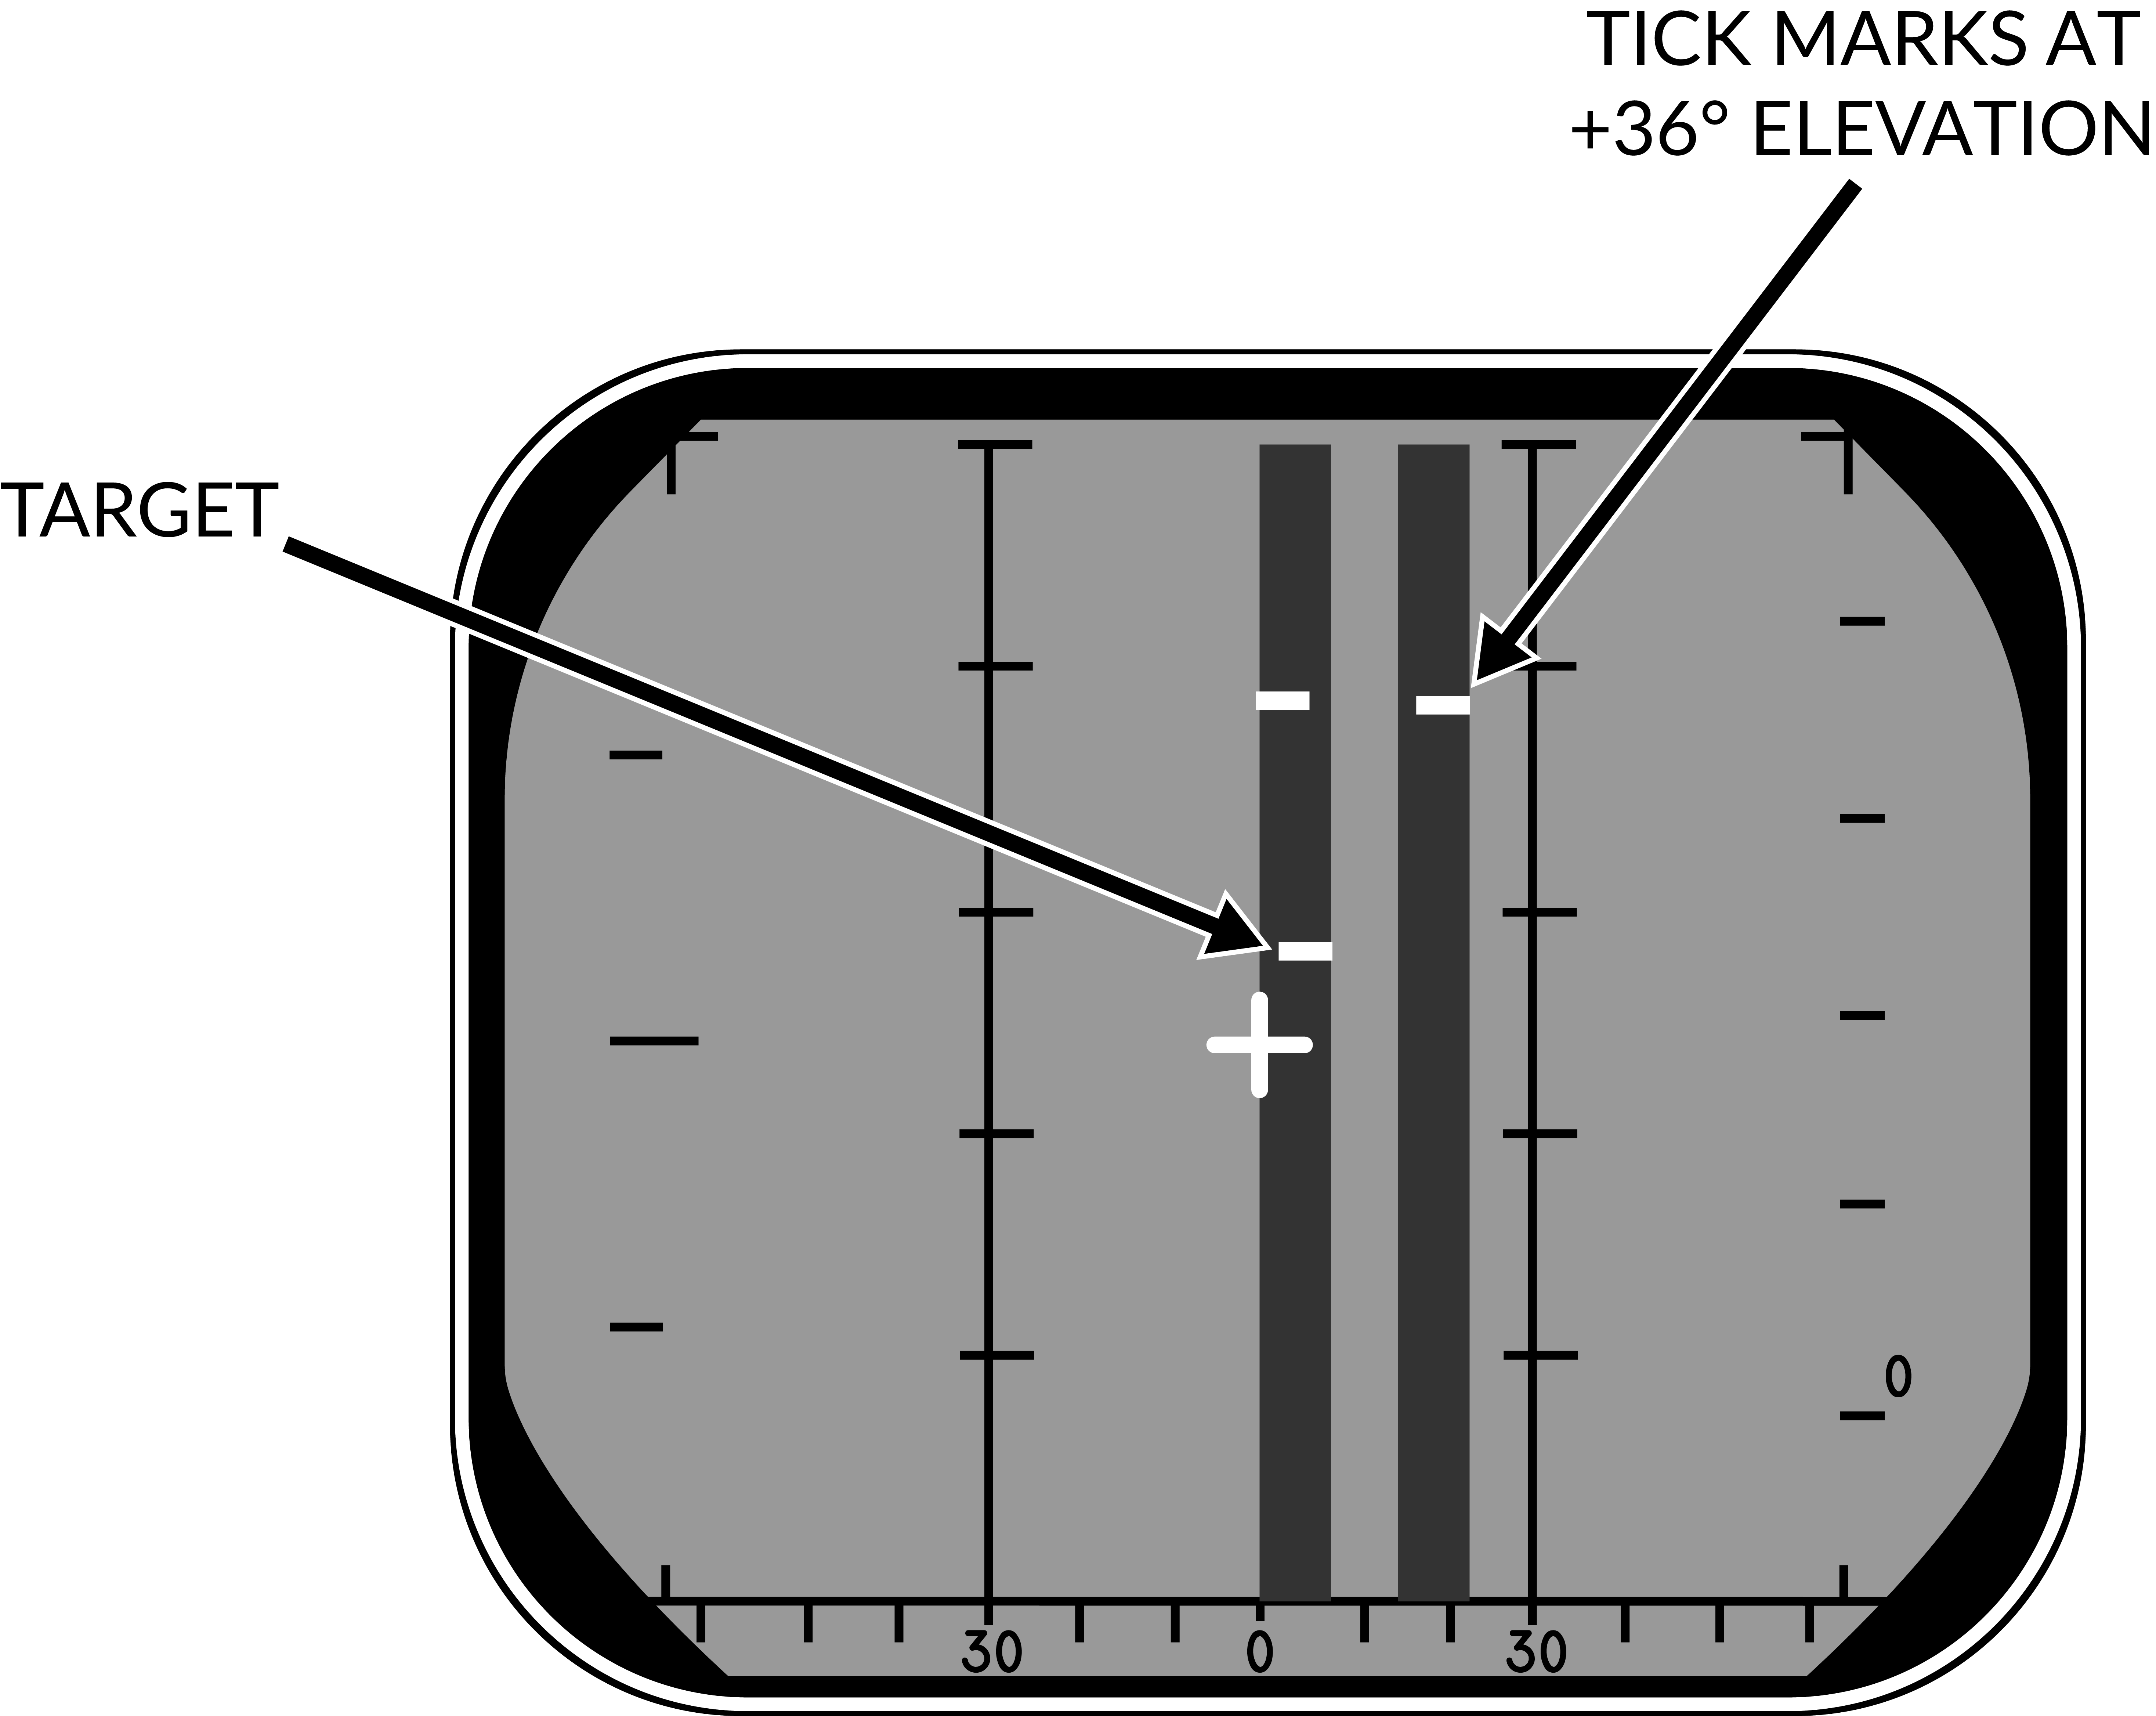
\includegraphics[width=\linewidth]{mrl.png}
			\subcaption{\textbf{DDD Format in MRL Mode}}
			\label{fig:acmvismrl}
		\end{subfigure}
		\begin{subfigure}[c]{0.43\linewidth}
			\centering
			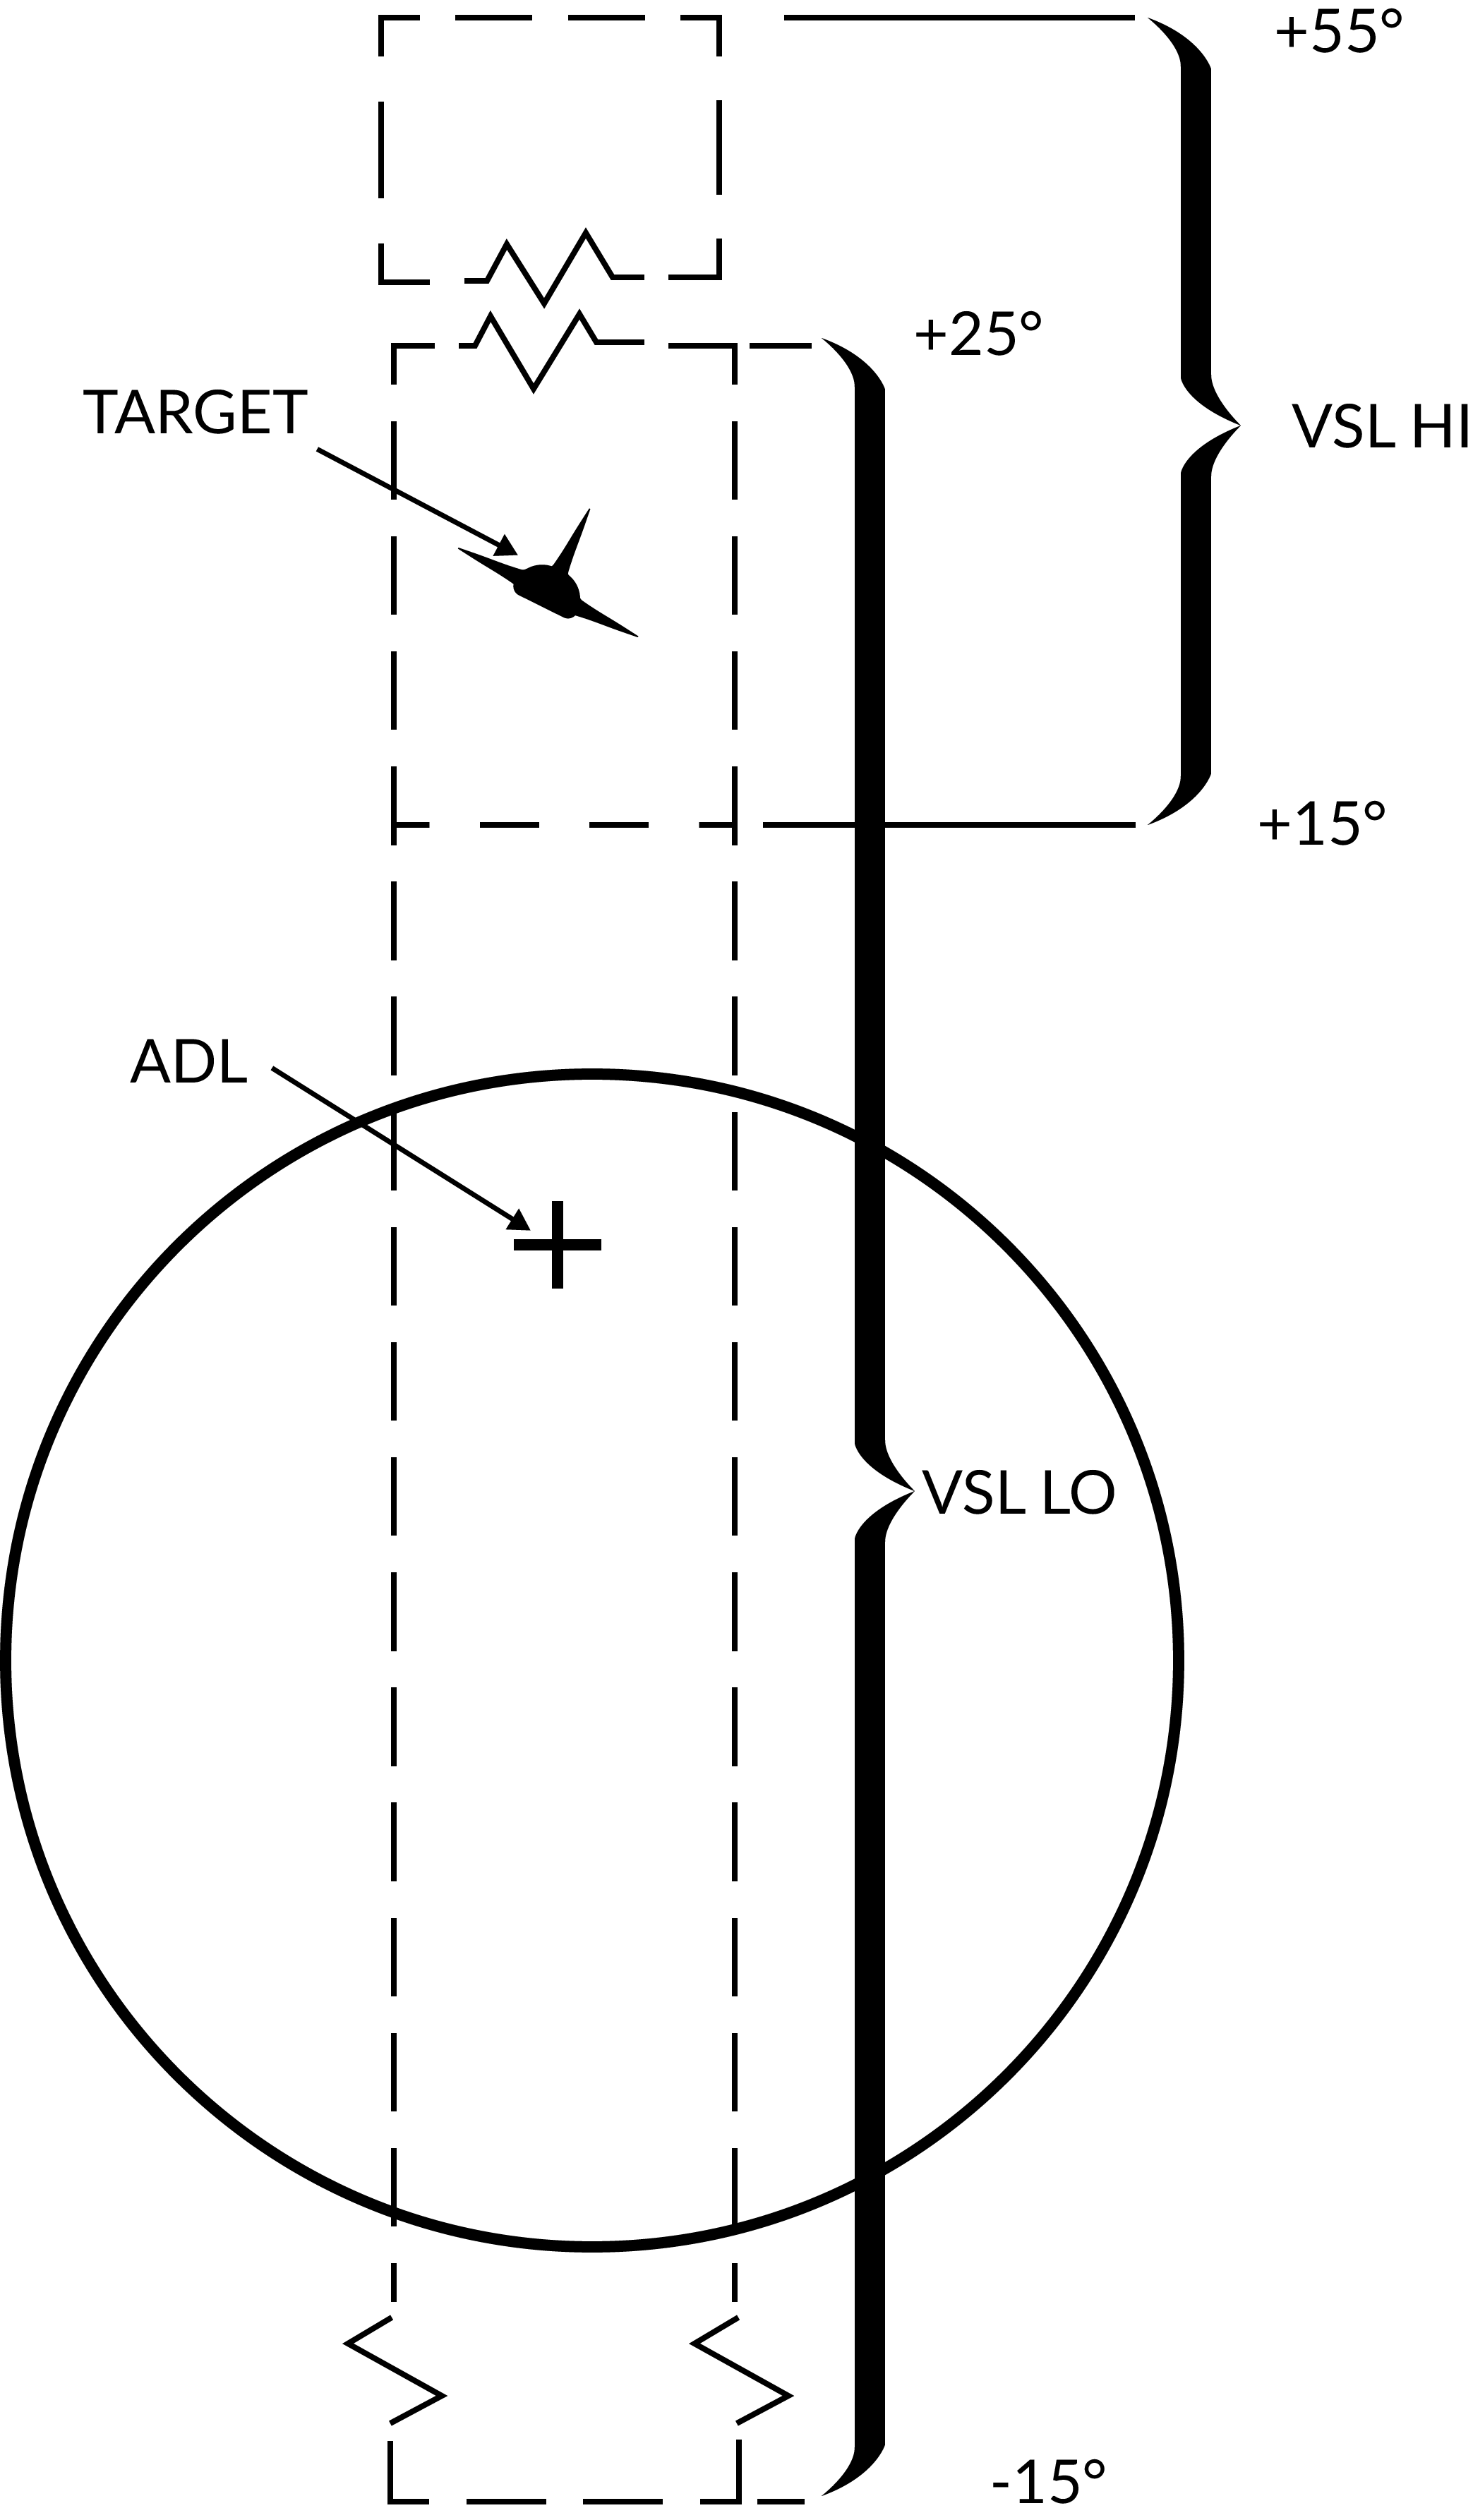
\includegraphics[width=\linewidth]{vsl.png}
			\subcaption{\textbf{VSL Search Patterns}}
			\label{fig:acmvisvsl}
		\end{subfigure}
		\caption{\textbf{ACM Search Mode Visualization}}
		\label{fig:acmvis}
	\end{figure}

	\clearpage 

	\section{APX-76 IFF}
	\subsection{OVERVIEW}
	\begin{tableitemize}
		\blueitem{Activation}{\textbf{IFF Switch} -- \textbf{Press \& Hold} (up to 10 sec)}
		\blueitem{Search Modes}{
			\begin{subitemize}
				\item \textbf{DDD} -- 2 horizontal bars above \& below all friendly returns
			\end{subitemize}
		}
		\blueitem{TWS / STT Modes}{
			\begin{subitemize}
				\item \textbf{DDD} -- 2 horizontal bars above \& below hooked / locked friendly 
				\item \textbf{DDD Range} -- shows \textbf{10 EXP}
			\end{subitemize}
		}
		\blueitem{Control Panel}{\textbf{Non-Functional in DCS} -- it \emph{just works}}
	\end{tableitemize}

	\notebox{
		\begin{itemize}
			\item \textbf{APX-76 Data is Not Correlated with TWS Tracks} -- RIO must manually enter target status (HOST, UNKN, FRIEND) via the \textbf{CAP}
			\item \textbf{Lack of IFF Return does NOT necessarily mean Hostile} 
			\item \textbf{APX-76 is a Secondary, Transponder-type Radar}
			\begin{itemize}
				\item Can receive IFF returns from targets not detected by AWG-9
			\end{itemize}
		\end{itemize}
	}



	\clearpage

	\section{TACTICAL INFORMATION DISPLAY}

	\subsection{TID SYMBOLOGY}
	\label{subsec:tidsymb}
	\begin{center}
		\begin{longtable}{p{3.5cm} | p{1cm} |  p{6cm}}
			\toprule
			\multicolumn{2}{c}{\blue{GENERAL}} &  \\
			\midrule
			\textbf{Center Dot} &
			\begin{minipage}[t]{\linewidth}
				\vspace{-7pt}
				\centering
				
\includegraphics[width=0.05cm]{1.png}
			\end{minipage} &
			\begin{minipage}[t]{\linewidth}
				\vspace{-7pt}
				\begin{itemize}
					\item \textbf{Basic Component of Symbols}
					\begin{itemize}
						\item Marks coordinates of symbol
					\end{itemize}
				\end{itemize}
			\end{minipage} \\
			\midrule
			\textbf{Own AC} &
			\begin{minipage}[t]{\linewidth}
				\vspace{-7pt}
				\centering
				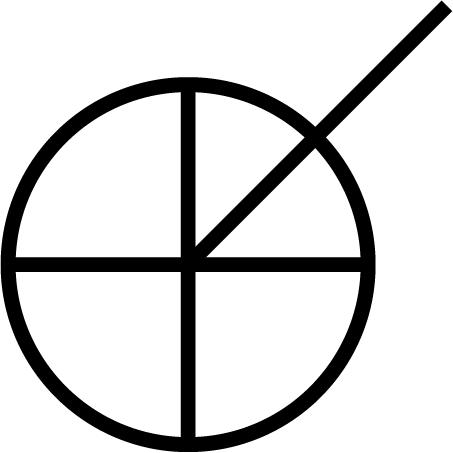
\includegraphics[width=0.8cm]{2.png}
			\end{minipage} &
			\begin{minipage}[t]{\linewidth}
				\vspace{-7pt}
				\begin{itemize}
					\item \textbf{Symbol representing own aircraft}
					\begin{itemize}
						\item Ground Stabilized: Moves
						\item Aircraft Stabilized: Stationary
						\item Outside TID: line drawn from TID center towards symbol
					\end{itemize}
				\end{itemize}
			\end{minipage} \\
			\midrule
			\textbf{TID Cursor} &
			\begin{minipage}[t]{\linewidth}
				\vspace{-7pt}
				\centering
				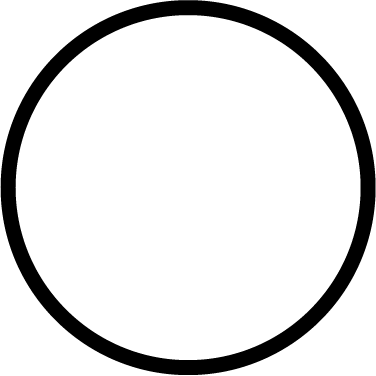
\includegraphics[width=0.8cm]{26.png}
			\end{minipage} &
			\begin{minipage}[t]{\linewidth}
				\vspace{-7pt}
				\begin{itemize}
					\item \textbf{Hook Cursor}
					\begin{itemize}
						\item Controlled by \textbf{HCU} in \textbf{TID mode}
					\end{itemize}
					\item \textbf{Half-Action}
					\begin{itemize}
						\item Enables display of symbol
						\item Enables HCU stick to move cursor
					\end{itemize}
					\item \textbf{Full-Action}
					\begin{itemize}
						\item Hooks closest symbol
						\item If no symbol near, cursor dropped at location
					\end{itemize}
				\end{itemize}
			\end{minipage} \\
			\midrule
			\textbf{TWS Steering Centroid} &
			\begin{minipage}[t]{\linewidth}
				\vspace{-7pt}
				\centering
				
\includegraphics[width=0.8cm]{27.png}
			\end{minipage} &
			\begin{minipage}[t]{\linewidth}
				\vspace{-7pt}
				\begin{itemize}
					\item \textbf{Steering centroid of TWS tracks}
					\begin{itemize}
						\item Selected by WCS for weapons engagement
					\end{itemize}
				\end{itemize}
			\end{minipage} \\
			\midrule
			\multicolumn{2}{c|}{\blue{ONBOARD SENSORS}} & \textbf{Symbol Above Dot} \\
			\midrule
			\textbf{Unknown} &
			\begin{minipage}[t]{\linewidth}
				\vspace{-7pt}
				\centering
				
\includegraphics[width=0.8cm]{3.png}
			\end{minipage} &
			\begin{minipage}[t]{\linewidth}
				\vspace{-7pt}
				\begin{itemize}
					\item \textbf{Unknown Sensor Track}
					\item \textbf{All Returns in RWS}
				\end{itemize}
			\end{minipage} \\
			\midrule
			\textbf{Hostile} &
			\begin{minipage}[t]{\linewidth}
				\vspace{-7pt}
				\centering
				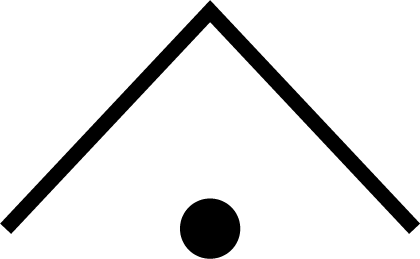
\includegraphics[width=0.8cm]{4.png}
			\end{minipage} &
			\begin{minipage}[t]{\linewidth}
				\vspace{-7pt}
				\begin{itemize}
					\item \textbf{Sensor Track designated Hostile by RIO}
				\end{itemize}
			\end{minipage} \\
			\midrule
			\textbf{Friend} &
			\begin{minipage}[t]{\linewidth}
				\vspace{-7pt}
				\centering
				
\includegraphics[width=0.8cm]{5.png}
			\end{minipage} &
			\begin{minipage}[t]{\linewidth}
				\vspace{-7pt}
				\begin{itemize}
					\item \textbf{Sensor Track designated Friendly by RIO}
				\end{itemize}
			\end{minipage} \\
			\midrule
			\textbf{Angle-Tracked Radar Target} &
			\begin{minipage}[t]{\linewidth}
				\vspace{-7pt}
				\centering
				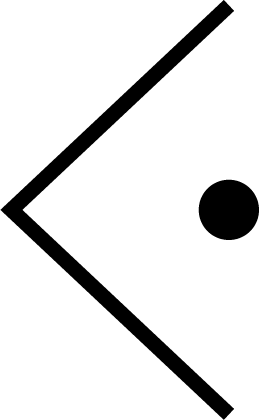
\includegraphics[width=0.55cm]{6.png}
			\end{minipage} &
			\begin{minipage}[t]{\linewidth}
				\vspace{-7pt}
				\begin{itemize}
					\item \textbf{Radar Angle Tracking}
					\begin{itemize}
						\item Jamming Target
					\end{itemize}
				\end{itemize}
			\end{minipage} \\
			\midrule
			\textbf{Angle-Tracked Radar Target with Altitude Difference Ranging} &
			\begin{minipage}[t]{\linewidth}
				\vspace{-7pt}
				\centering
				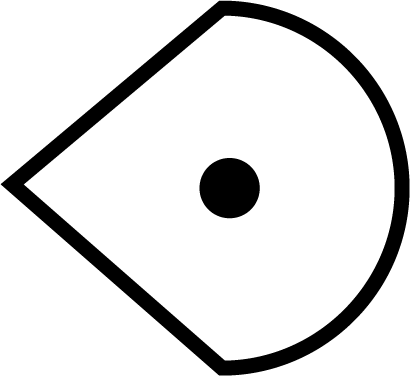
\includegraphics[width=0.8cm]{7.png}
			\end{minipage} &
			\begin{minipage}[t]{\linewidth}
				\vspace{-7pt}
				\begin{itemize}
					\item \textbf{Radar Angle Tracking}
					\begin{itemize}
						\item Jamming Target
						\item Alt. diff. ranging
					\end{itemize}
				\end{itemize}
			\end{minipage} \\
			\midrule
			\textbf{TCS-Angle Tracked Target} &
			\begin{minipage}[t]{\linewidth}
				\vspace{-7pt}
				\centering
				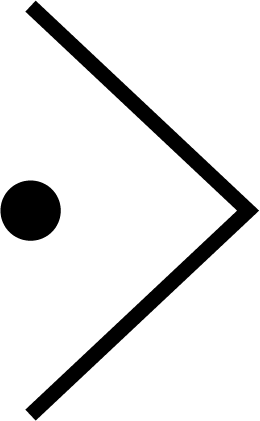
\includegraphics[width=0.55cm]{10.png}
			\end{minipage} &
			\begin{minipage}[t]{\linewidth}
				\vspace{-7pt}
				\begin{itemize}
					\item \textbf{TCS Angle Tracking}
				\end{itemize}
			\end{minipage} \\
			\midrule
			\textbf{TCS-Angle Tracked Target with Altitude Difference Ranging} &
			\begin{minipage}[t]{\linewidth}
				\vspace{-7pt}
				\centering
				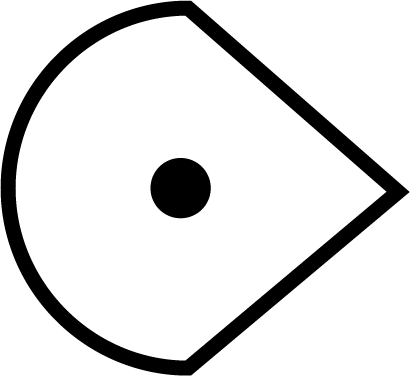
\includegraphics[width=0.8cm]{11.png}
			\end{minipage} &
			\begin{minipage}[t]{\linewidth}
				\vspace{-7pt}
				\begin{itemize}
					\item \textbf{TCS Angle Tracking}
					\begin{itemize}
						\item Alt. diff. ranging
					\end{itemize}
				\end{itemize}
			\end{minipage} \\
			\midrule
			\multicolumn{2}{c|}{\blue{D/L TARGETS}} & \textbf{Symbol Below Dot} \\
			\midrule
			\textbf{Unknown} &
			\begin{minipage}[t]{\linewidth}
				\vspace{-7pt}
				\centering
				
\includegraphics[width=0.8cm]{12.png}
			\end{minipage} &
			\begin{minipage}[t]{\linewidth}
				\vspace{-7pt}
				\begin{itemize}
					\item \textbf{D/L Track designated Unknown by Source}
				\end{itemize}
			\end{minipage} \\
			\midrule
			\textbf{Hostile} &
			\begin{minipage}[t]{\linewidth}
				\vspace{-7pt}
				\centering
				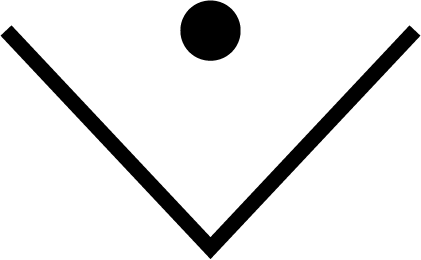
\includegraphics[width=0.8cm]{13.png}
			\end{minipage} &
			\begin{minipage}[t]{\linewidth}
				\vspace{-7pt}
				\begin{itemize}
					\item \textbf{D/L Track designated Hostile by Source}
				\end{itemize}
			\end{minipage} \\
			\midrule
			\textbf{Friendly} &
			\begin{minipage}[t]{\linewidth}
				\vspace{-7pt}
				\centering
				
\includegraphics[width=0.8cm]{14.png}
			\end{minipage} &
			\begin{minipage}[t]{\linewidth}
				\vspace{-7pt}
				\begin{itemize}
					\item \textbf{D/L Track designated Friendly by Source}
				\end{itemize}
			\end{minipage} \\
			\midrule
			\multicolumn{2}{c}{\blue{MANUAL REF POINTS}} & \\
			\midrule
			\textbf{Home base} &
			\begin{minipage}[t]{\linewidth}
				\vspace{-7pt}
				\centering
				
\includegraphics[width=0.8cm]{15.png}
			\end{minipage} &
			\begin{minipage}[t]{\linewidth}
				\vspace{-7pt}
				\begin{itemize}
					\item \textbf{Waypoint Representing}
					\begin{itemize}
						\item Home Base
						\item Carrier
						\item Airfield
					\end{itemize}
				\end{itemize}
			\end{minipage} \\
			\midrule
			\textbf{Waypoint} &
			\begin{minipage}[t]{\linewidth}
				\vspace{-7pt}
				\centering
				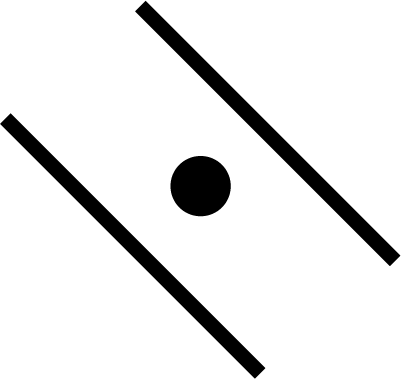
\includegraphics[width=0.8cm]{16.png}
			\end{minipage} &
			\begin{minipage}[t]{\linewidth}
				\vspace{-7pt}
				\begin{itemize}
					\item \textbf{Nav Waypoint}
					\item \textbf{Supplanted by Number}
					\begin{itemize}
						\item 1, 2, or 3
					\end{itemize}
				\end{itemize}
			\end{minipage} \\
			\midrule
			\textbf{Defended Point} &
			\begin{minipage}[t]{\linewidth}
				\vspace{-7pt}
				\centering
				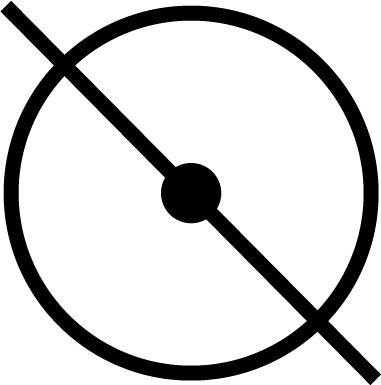
\includegraphics[width=0.8cm]{17.png}
			\end{minipage} &
			\begin{minipage}[t]{\linewidth}
				\vspace{-7pt}
				\begin{itemize}
					\item \textbf{Waypoint to Defend}
				\end{itemize}
			\end{minipage} \\
			\midrule
			\textbf{Fixed Point} &
			\begin{minipage}[t]{\linewidth}
				\vspace{-7pt}
				\centering
				
\includegraphics[width=0.8cm]{18.png}
			\end{minipage} &
			\begin{minipage}[t]{\linewidth}
				\vspace{-7pt}
				\begin{itemize}
					\item \textbf{Generic Waypoint}
				\end{itemize}
			\end{minipage} \\
			\midrule
			\textbf{Hostile Area} &
			\begin{minipage}[t]{\linewidth}
				\vspace{-7pt}
				\centering
				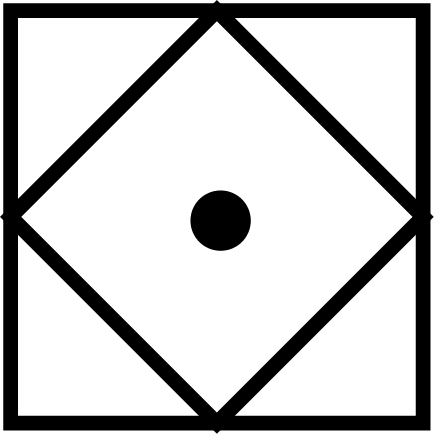
\includegraphics[width=0.8cm]{19.png}
			\end{minipage} &
			\begin{minipage}[t]{\linewidth}
				\vspace{-7pt}
				\begin{itemize}
					\item \textbf{Waypoint Indicating Hostile Area}
				\end{itemize}
			\end{minipage} \\
			\midrule
			\textbf{Surface Target} &
			\begin{minipage}[t]{\linewidth}
				\vspace{-7pt}
				\centering
				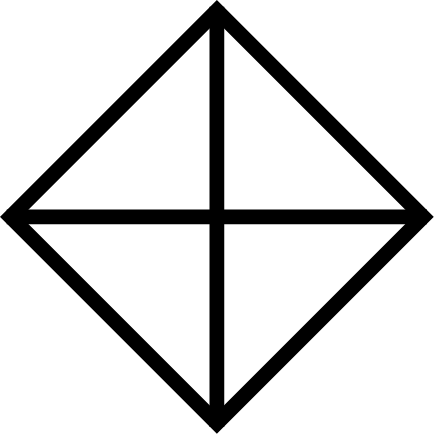
\includegraphics[width=0.8cm]{20.png}
			\end{minipage} &
			\begin{minipage}[t]{\linewidth}
				\vspace{-7pt}
				\begin{itemize}
					\item \textbf{Waypoint Indicating Surface Target}
				\end{itemize}
			\end{minipage} \\
			\midrule
			\textbf{IP} &
			\begin{minipage}[t]{\linewidth}
				\vspace{-7pt}
				\centering
				
\includegraphics[width=0.8cm]{21.png}
			\end{minipage} &
			\begin{minipage}[t]{\linewidth}
				\vspace{-7pt}
				\begin{itemize}
					\item \textbf{Initial Point}
					\begin{itemize}
						\item Waypoint for A/G engagement
					\end{itemize}
				\end{itemize}
			\end{minipage} \\
			\midrule
			\multicolumn{2}{c}{\blue{D/L REF POINTS}} & \\
			\midrule
			\textbf{Home Base} &
			\begin{minipage}[t]{\linewidth}
				\vspace{-7pt}
				\centering
				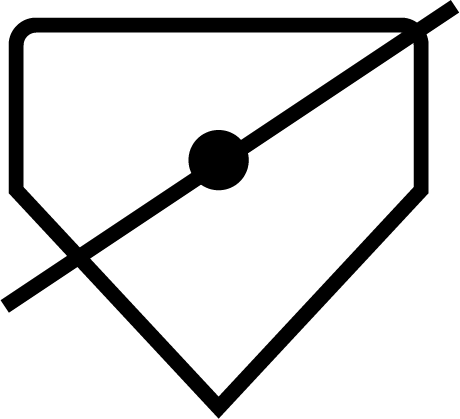
\includegraphics[width=0.8cm]{22.png}
			\end{minipage} &
			\begin{minipage}[t]{\linewidth}
				\vspace{-7pt}
				\begin{itemize}
					\item \textbf{D/L Waypoint Representing Home Base}
				\end{itemize}
			\end{minipage} \\
			\midrule
			\textbf{Waypoint} &
			\begin{minipage}[t]{\linewidth}
				\vspace{-7pt}
				\centering
				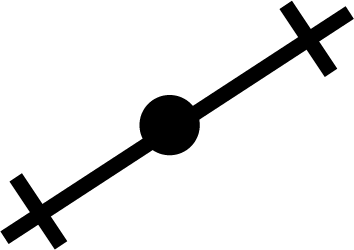
\includegraphics[width=0.8cm]{23.png}
			\end{minipage} &
			\begin{minipage}[t]{\linewidth}
				\vspace{-7pt}
				\begin{itemize}
					\item \textbf{D/L Generic Waypoint}
				\end{itemize}
			\end{minipage} \\
			\midrule
			\textbf{Data Link Fixed Point} &
			\begin{minipage}[t]{\linewidth}
				\vspace{-7pt}
				
\includegraphics[width=0.8cm]{24.png}
			\end{minipage} &
			\begin{minipage}[t]{\linewidth}
				\vspace{-7pt}
				\begin{itemize}
					\item \textbf{D/L Waypoint Representing Fixed Point}
				\end{itemize}
			\end{minipage} \\
			\midrule
			\textbf{Surface Target} &
			\begin{minipage}[t]{\linewidth}
				\vspace{-7pt}
				\centering
				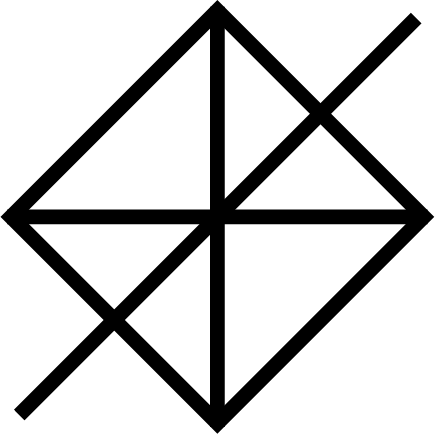
\includegraphics[width=0.8cm]{25.png}
			\end{minipage} &
			\begin{minipage}[t]{\linewidth}
				\vspace{-7pt}
				\begin{itemize}
					\item \textbf{D/L Waypoint Representing a Surface Target}
				\end{itemize}
			\end{minipage} \\
			\midrule
			\multicolumn{2}{c}{\blue{POS SYMB MODIFIERS}} &  \\
			\midrule
			\textbf{Mandatory Attack} &
			\begin{minipage}[t]{\linewidth}
				\vspace{-7pt}
				\centering
				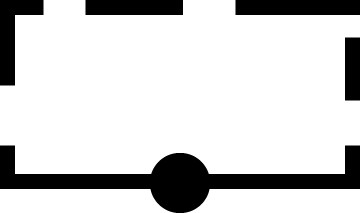
\includegraphics[width=0.8cm]{28.png}
			\end{minipage} &
			\begin{minipage}[t]{\linewidth}
				\vspace{-7pt}
				\begin{itemize}
					\item \textbf{Additional Symbology on TWS Track}
					\begin{itemize}
						\item Horizontal bar through center dot
					\end{itemize}
					\item \textbf{Selected by RIO}
					\begin{itemize}
						\item Only 1 target can be designated
						\item Guaranteed WCS priority number
					\end{itemize}
				\end{itemize}
			\end{minipage} \\
			\midrule
			\textbf{Data Link Destroy }&
			\begin{minipage}[t]{\linewidth}
				\vspace{-7pt}
				\centering
				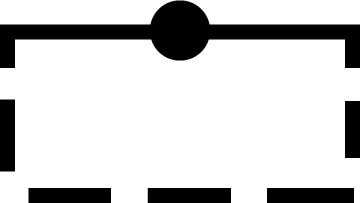
\includegraphics[width=0.8cm]{29.png}
			\end{minipage} &
			\begin{minipage}[t]{\linewidth}
				\vspace{-7pt}
				\begin{itemize}
					\item \textbf{Additional Symbology on D/L Track}
					\begin{itemize}
						\item Horizontal bar through center dot
					\end{itemize}
					\item \textbf{Selected by Source}
					\begin{itemize}
						\item No effect on WCS prioritization
					\end{itemize}
				\end{itemize}
			\end{minipage} \\
			\midrule
			\textbf{Do Not Attack} &
			\begin{minipage}[t]{\linewidth}
				\vspace{-7pt}
				\centering
				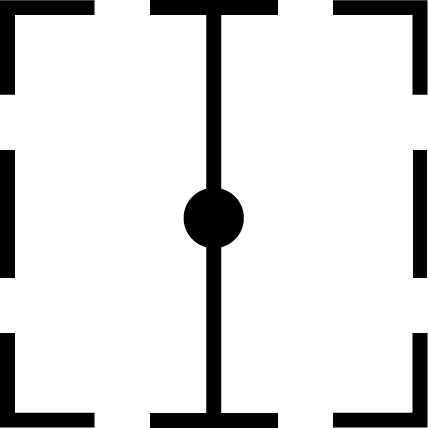
\includegraphics[width=0.8cm]{30.png}
			\end{minipage} &
			\begin{minipage}[t]{\linewidth}
				\vspace{-7pt}
				\begin{itemize}
					\item \textbf{Additional Symbology on TWS or D/L Track}
					\begin{itemize}
						\item Vertical bar through center dot
					\end{itemize}
					\item \textbf{If Set by RIO}
					\begin{itemize}
						\item Removes WCS prioritization
					\end{itemize}
				\end{itemize}
			\end{minipage} \\
			\midrule
			\textbf{Multiple Targets} &
			\begin{minipage}[t]{\linewidth}
				\vspace{-7pt}
				\centering
				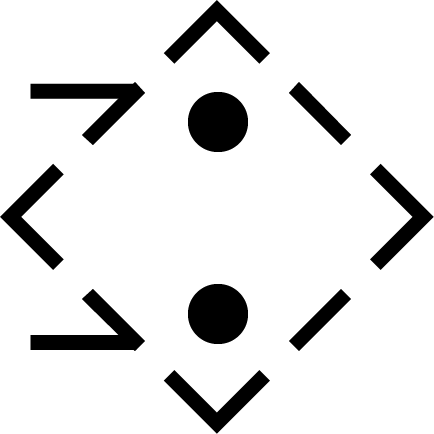
\includegraphics[width=0.8cm]{31.png}
			\end{minipage} &
			\begin{minipage}[t]{\linewidth}
				\vspace{-7pt}
				\begin{itemize}
					\item \textbf{Additional Symbology on TWS or D/L Track}
					\begin{itemize}
						\item Horizontal bar on left side of symbol
					\end{itemize}
					\item \textbf{Indicates Multiple Targets}
				\end{itemize}
			\end{minipage} \\
			\midrule
			\textbf{Data Link Challenge} &
			\begin{minipage}[t]{\linewidth}
				\vspace{-7pt}
				\centering
				
\includegraphics[width=0.8cm]{32.png}
			\end{minipage} &
			\begin{minipage}[t]{\linewidth}
				\vspace{-7pt}
				\begin{itemize}
					\item \textbf{Additional Symbology on D/L Track}
					\begin{itemize}
						\item Small \textbf{V} with center at center dot
					\end{itemize}
					\item \textbf{Command to Visually Identify}
				\end{itemize}
			\end{minipage} \\
			\midrule
			\textbf{Track Extrapolated} &
			\begin{minipage}[t]{\linewidth}
				\vspace{-7pt}
				\centering
				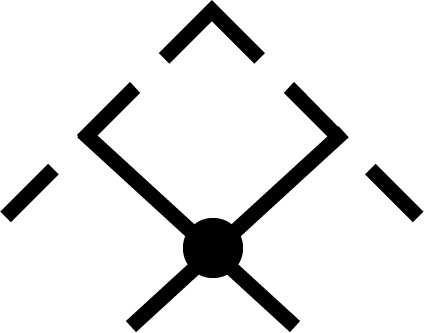
\includegraphics[width=0.8cm]{33.png}
			\end{minipage} &
			\begin{minipage}[t]{\linewidth}
				\vspace{-7pt}
				\begin{itemize}
					\item \textbf{Additional Symbology on TWS or D/L Track}
					\begin{itemize}
						\item Small \textbf{X} with center at center dot
					\end{itemize}
					\item \textbf{No Update within 8 seconds}
					\begin{itemize}
						\item Track deleted after 14 seconds
						\item Or after 2 min if track hold
					\end{itemize}
				\end{itemize}
			\end{minipage} \\
			\midrule
			\textbf{Altitude Numerics} &
			\begin{minipage}[t]{\linewidth}
				\vspace{-7pt}
				\centering
				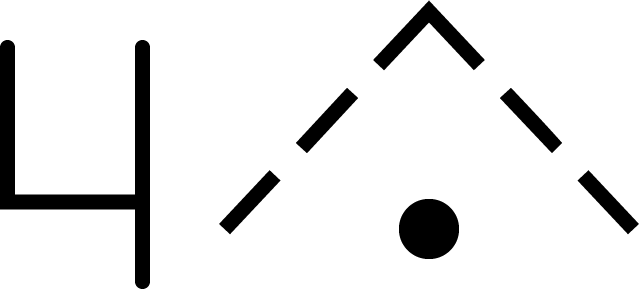
\includegraphics[width=1cm]{34.png}
			\end{minipage} &
			\begin{minipage}[t]{\linewidth}
				\vspace{-7pt}
				\begin{itemize}
					\item \textbf{Altitude to Nearest Ten Thousand}
					\begin{itemize}
						\item example: 35000-45000
					\end{itemize}
				\end{itemize}
			\end{minipage} \\
			\midrule
			\textbf{Firing Order Numerics} &
			\begin{minipage}[t]{\linewidth}
				\vspace{-7pt}
				\centering
				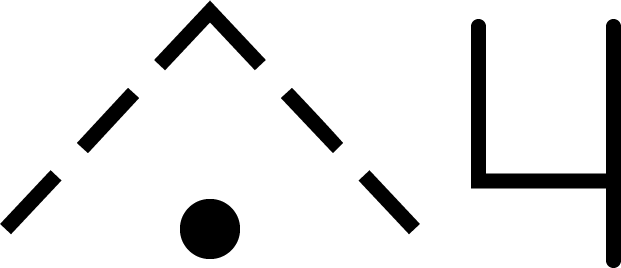
\includegraphics[width=1cm]{35.png}
			\end{minipage} &
			\begin{minipage}[t]{\linewidth}
				\vspace{-7pt}
				\begin{itemize}
					\item \textbf{Indicates AIM-54 Prioritization}
					\begin{itemize}
						\item Numbers 1-6
						\item Only in TWS
					\end{itemize}
				\end{itemize}
			\end{minipage} \\
			\midrule
			\textbf{Time-to-Impact (TTI)} &
			\begin{minipage}[t]{\linewidth}
				\vspace{-7pt}
				\centering
				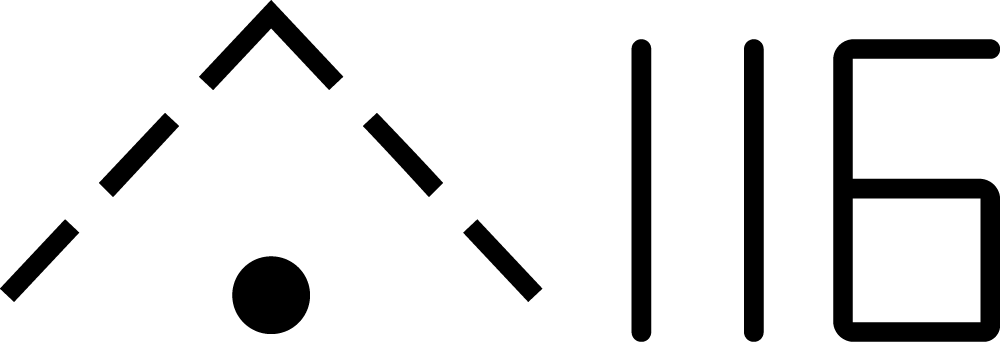
\includegraphics[width=1cm]{47.png}
			\end{minipage} &
			\begin{minipage}[t]{\linewidth}
				\vspace{-7pt}
				\begin{itemize}
					\item \textbf{After AIM-54 Launch}
					\begin{itemize}
						\item Prioritization replaced with estimated TTI
					\end{itemize}
					\item \textbf{Flashes after Pitbull}
				\end{itemize}
			\end{minipage} \\
			\midrule
			\textbf{Velocity Vector} &
			\begin{minipage}[t]{\linewidth}
				\vspace{-7pt}
				\centering
				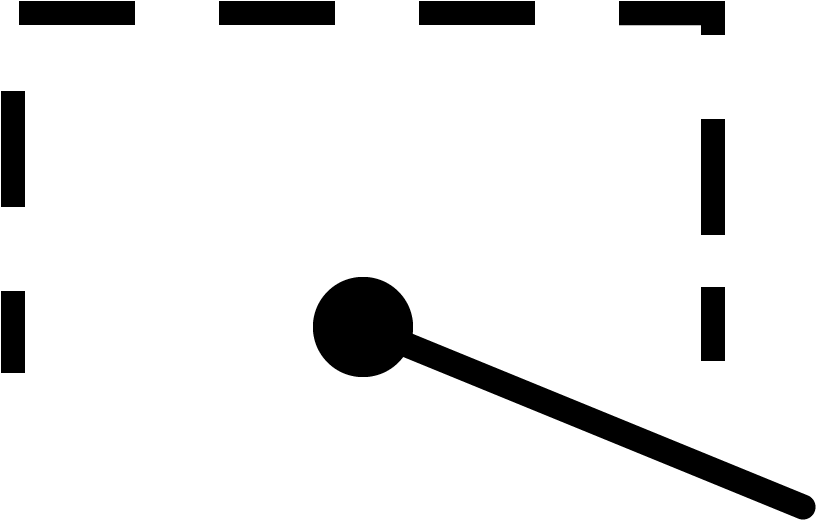
\includegraphics[width=0.8cm]{36.png}
			\end{minipage} &
			\begin{minipage}[t]{\linewidth}
				\vspace{-7pt}
				\begin{itemize}
					\item \textbf{Additional Symbology from center Dot}
					\begin{itemize}
						\item Direction represents track heading
						\item Length represents speed
					\end{itemize}
					\item \textbf{Varies with Mode}
					\begin{itemize}
						\item Ground Stabilized: true heading and ground speed
						\item Aircraft Stabilized: relative heading and velocity
					\end{itemize}
				\end{itemize}
			\end{minipage} \\
			\midrule
			\textbf{Launch Zone Vectors} &
			\begin{minipage}[t]{\linewidth}
				\vspace{-7pt}
				\centering
				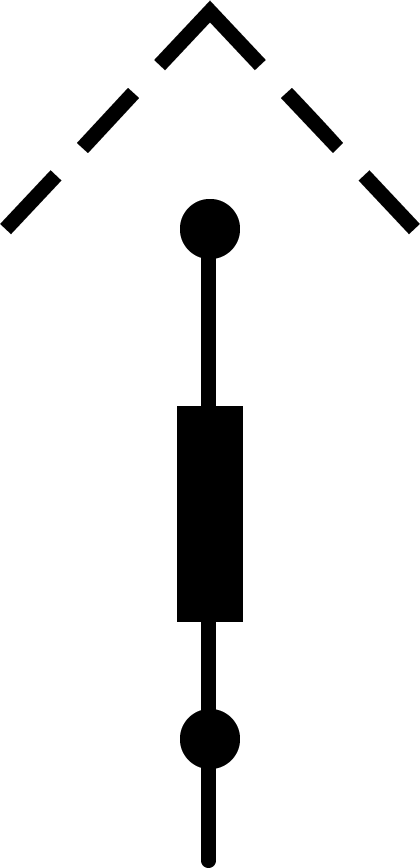
\includegraphics[width=0.8cm]{37.png}
			\end{minipage} &
			\begin{minipage}[t]{\linewidth}
				\vspace{-7pt}
				\centering
				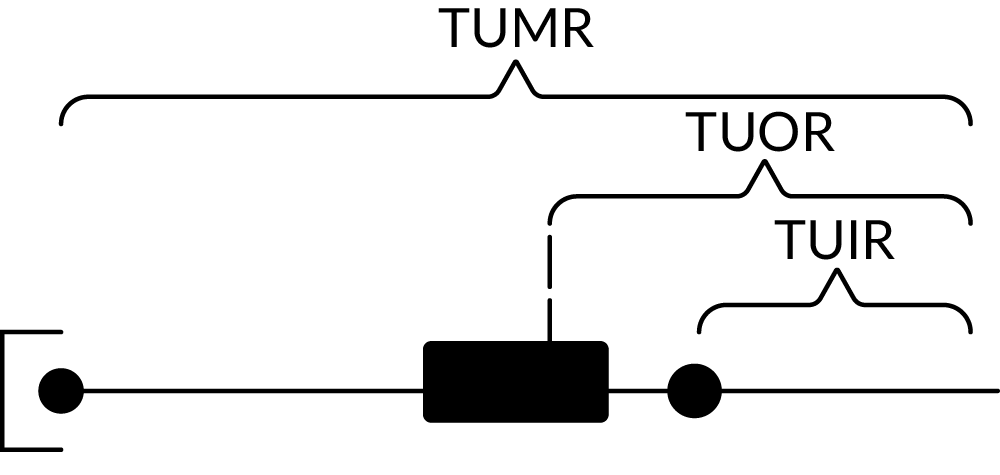
\includegraphics[width=5cm]{lzv.png}
			\end{minipage}
			\begin{minipage}[t]{\linewidth}
				\begin{itemize}
					\item \textbf{Additional Symbology for AIM-54}
					\begin{itemize}
						\item Selected manually by RIO
						\item Or 60 seconds from max launch
					\end{itemize}
					\item \textbf{TUMR}
					\begin{itemize}
						\item Time-Until-Minimum-Range
						\item Max: 180 seconds, 1.5 inches
					\end{itemize}
					\item \textbf{TUOR}
					\begin{itemize}
						\item Time-Until-Optimal-Range
						\item Start of bar is 8 seconds from optimum
					\end{itemize}
					\item \textbf{TUIR}
					\begin{itemize}
						\item Time-Until-In-Range
					\end{itemize}
				\end{itemize}
			\end{minipage} \\
			\midrule
			\textbf{Jamming Strobe} &
			\begin{minipage}[t]{\linewidth}
				\vspace{-7pt}
				\centering
				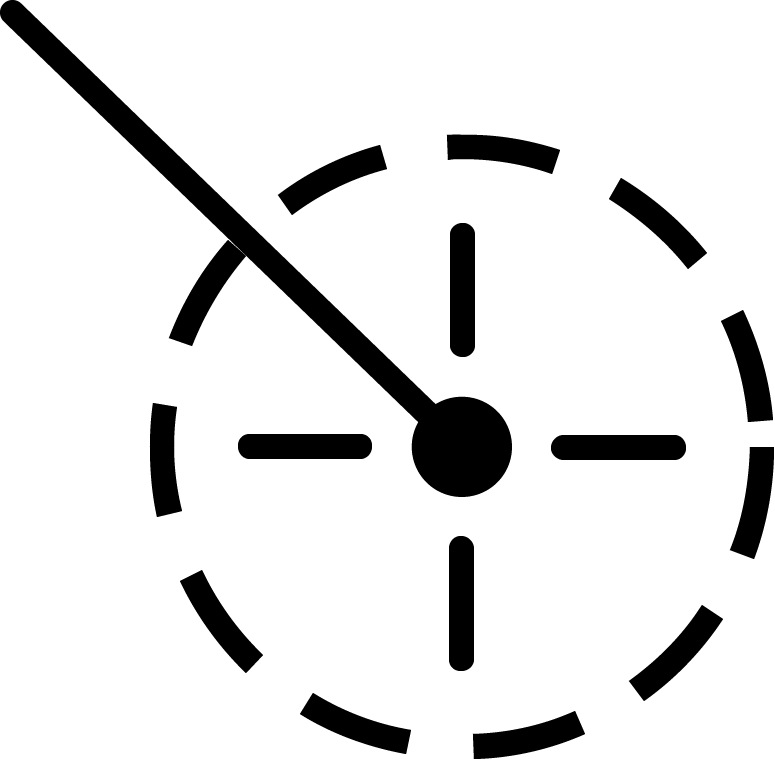
\includegraphics[width=0.8cm]{38.png}
			\end{minipage} &
			\begin{minipage}[t]{\linewidth}
				\vspace{-7pt}
				\begin{itemize}
					\item \textbf{Line from own AC towards Jammer}
				\end{itemize}
			\end{minipage} \\
			\midrule
			\textbf{Radar Antenna Scan Pattern Azimuth Limit}s &
			\begin{minipage}[t]{\linewidth}
				\vspace{-7pt}
				\centering
				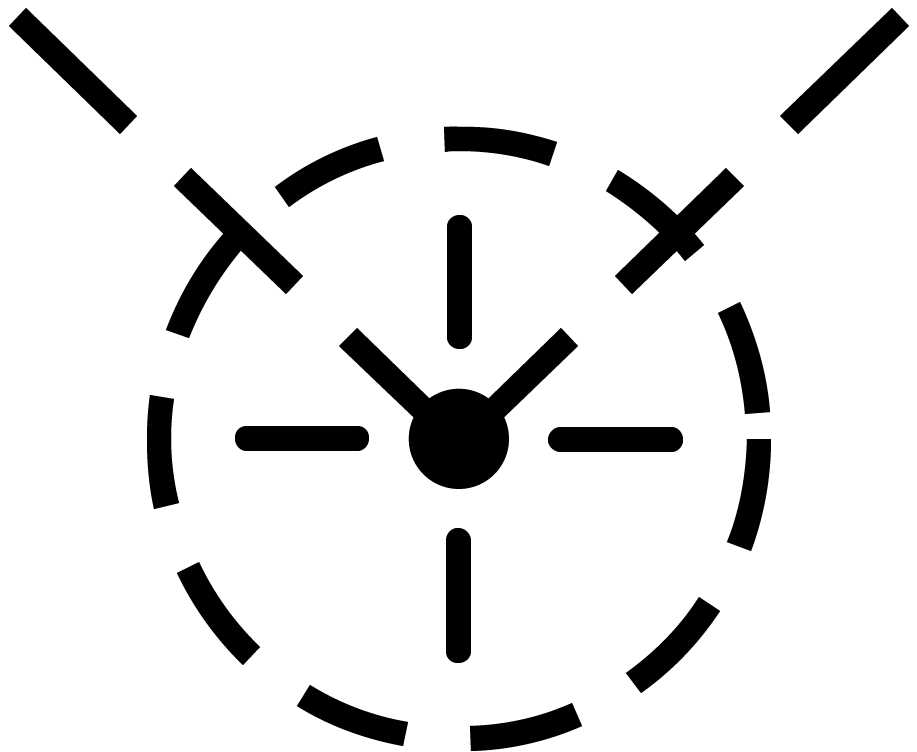
\includegraphics[width=0.8cm]{39.png}
			\end{minipage} &
			\begin{minipage}[t]{\linewidth}
				\vspace{-7pt}
				\begin{itemize}
					\item \textbf{Limits of Current Scan Azimuth}
					\item \textbf{Single Line in STT}
				\end{itemize}
			\end{minipage} \\
			\midrule
			\textbf{Data Link Jamming Strobe} &
			\begin{minipage}[t]{\linewidth}
				\vspace{-7pt}
				\centering
				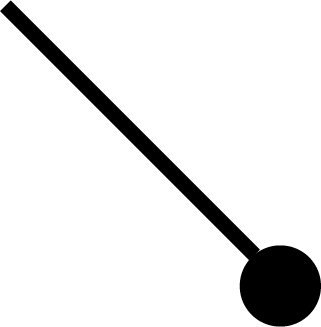
\includegraphics[width=0.8cm]{40.png}
			\end{minipage} &
			\begin{minipage}[t]{\linewidth}
				\vspace{-7pt}
				\begin{itemize}
					\item \textbf{Line from D/L point towards Jammer}
				\end{itemize}
			\end{minipage} \\
			\midrule
			\textbf{Data Link Pointer} &
			\begin{minipage}[t]{\linewidth}
				\vspace{-7pt}
				\centering
				\includegraphics[width=0.8cm]{41.png}
			\end{minipage} &
			\begin{minipage}[t]{\linewidth}
				\vspace{-7pt}
				\begin{itemize}
					\item \textbf{Additional Symbology on D/L Track}
					\begin{itemize}
						\item Circle
						\item Indicates operator concern
					\end{itemize}
				\end{itemize}
			\end{minipage} \\
			\midrule
			\textbf{Data Link Priority Kill} &
			\begin{minipage}[t]{\linewidth}
				\vspace{-7pt}
				\centering
				\includegraphics[width=0.8cm]{42.png}
			\end{minipage} &
			\begin{minipage}[t]{\linewidth}
				\vspace{-7pt}
				\begin{itemize}
					\item \textbf{Additional Symbology on D/L Track}
					\begin{itemize}
						\item Square
						\item Indicates target must be destroyed
						\item No effect on WCS prioritization
					\end{itemize}
				\end{itemize}
			\end{minipage} \\
			\midrule
			\multicolumn{2}{c}{\blue{ATTACK DISPLAY SYMBOLOGY}} & \\
			\midrule
			\textbf{Artificial Horizon} &
			\begin{minipage}[t]{\linewidth}
				\vspace{-7pt}
				\centering
				\includegraphics[width=0.8cm]{43.png}
			\end{minipage} &
			\begin{minipage}[t]{\linewidth}
				\vspace{-7pt}
				\begin{itemize}
					\item \textbf{Represents Pitch and Roll}
				\end{itemize}
			\end{minipage} \\
			\midrule
			\textbf{Steering Guidance Symbol} &
			\begin{minipage}[t]{\linewidth}
				\vspace{-7pt}
				\centering
				\includegraphics[width=0.8cm]{44.png}
			\end{minipage} &
			\begin{minipage}[t]{\linewidth}
				\vspace{-7pt}
				\begin{itemize}
					\item \textbf{Represents Steering Error}
					\begin{itemize}
						\item Should be placed as near as possible to center of ASE circle
					\end{itemize}
				\end{itemize}
			\end{minipage} \\
			\midrule
			\textbf{Allowable Steering Error Circle} &
			\begin{minipage}[t]{\linewidth}
				\vspace{-7pt}
				\centering
				\includegraphics[width=0.8cm]{45.png}
			\end{minipage} &
			\begin{minipage}[t]{\linewidth}
				\vspace{-7pt}
				\begin{itemize}
					\item \textbf{Indicates Allowable Steering Error for Missile Launch}
					\item \textbf{Size Varies with Geometry, Mode, Missile}
				\end{itemize}
			\end{minipage} \\
			\midrule
			\textbf{Breakaway Indication} &
			\begin{minipage}[t]{\linewidth}
				\vspace{-7pt}
				\centering
				\includegraphics[width=0.8cm]{27.png}
			\end{minipage} &
			\begin{minipage}[t]{\linewidth}
				\vspace{-7pt}
				\begin{itemize}
					\item \textbf{Appears when Target Range Less than Minimum for Selected Weapon}
				\end{itemize}
			\end{minipage} \\
			\bottomrule
		\end{longtable}
	\end{center}

	\cleardoublepage

	\chapter{TCS - LANTIRN}
	\thumbtab{TCS - LANTIRN}{3}
	\minitoc
	\cleardoublepage

	\section{TCS}


	\subsection{OVERVIEW}

	\cleardoublepage

	\section{LANTIRN}

	\subsection{OVERVIEW}
	\begin{tableitemize}
		\blueitem{LANTIRN}{\textbf{L}ow \textbf{A}ltitude \textbf{N}avigation and \textbf{T}argeting \textbf{I}nfra-\textbf{R}ed for \textbf{N}ight
		\begin{subitemize}
			\item \textbf{Only Targeting Pod} -- Nav pod was deleted
			\item \textbf{Incomplete Integration} -- Own control panel, supplants TCS feed
		\end{subitemize}}
		\blueitem{Master Modes}{
		\begin{subitemize}
			\item \textbf{A/G} -- Allows bomb release guidance
			\item \textbf{A/A} -- Optimized for air targets
		\end{subitemize}}
		\blueitem{FOV Levels \break Overview}{
		\begin{subitemize}
			\item \textbf{Wide}
			\begin{itemize}
				\item \textbf{FOV} -- 5.9 deg
				\item \textbf{Slew} -- 8.5 deg/s
			\end{itemize}
			\item \textbf{Narrow}
			\begin{itemize}
				\item \textbf{FOV} -- 1.7 deg
				\item \textbf{Slew} -- 1.8 deg/s
			\end{itemize}
			\item \textbf{Expanded}
			\begin{itemize}
				\item \textbf{FOV} -- 0.8 deg
				\item \textbf{Slew} -- 0.7 deg/s
				\item \textbf{Digital Zoom} -- Degraded quality
			\end{itemize}
		\end{subitemize}}
	\end{tableitemize}

	\subsection{OVERVIEW - STARTUP}
	\begin{tablenumerate}
		\dblueitem{Power Switch}{\textbf{POD}}
		\blueitem{Pod Startup Sequence}{		
		\begin{subitemize}
			\item 8 min startup sequence
			\item \textbf{MODE Switch} shows \textbf{STBY} when complete
		\end{subitemize}}
		\dblueitem{MODE Switch}{\textbf{Press}}
		\blueitem{Initialization Sequence}{		
		\begin{subitemize}
			\item 30 sec initialization
			\item \textbf{MODE Switch} shows \textbf{OPER} when ready
		\end{subitemize}}
		\dblueitem{VIDEO Switch}{\textbf{FLIR}}
		\dblueitem{TID MODE}{\textbf{TV}}
	\end{tablenumerate}

	\clearpage

	\subsection{OVERVIEW - POINTING MODES}
	\begin{tableitemize}
		\blueitem{Sensor Modes Overview}{
		\begin{subitemize}
			\item \textbf{Contrast Lock}
			\begin{itemize}
				\item \textbf{Area Track}
				\item \textbf{Point Track}
			\end{itemize}
			\item \textbf{Q Designation}
			\begin{itemize}
				\item \textbf{Directional Q} -- QSNO / QADL / QHUD
				\item \textbf{Location Q} -- QWp / QDES
			\end{itemize}
		\end{subitemize}}
		\blueitem{Directional Q}{
		\begin{subitemize}
			\item \textbf{Do Not Allow Weapon Guidance}
			\item \textbf{QSNO}
			\begin{itemize}
				\item Pod slaved to \textbf{ground 15 nm in front} along own aircraft heading
			\end{itemize}
			\item \textbf{QADL}
			\begin{itemize}
				\item \textbf{Pod slaved to ADL}
				\item In A/A mode
			\end{itemize}
			\item \textbf{QHUD}
			\begin{itemize}
				\item \textbf{Pod slaved to HUD}
				\item In A/G mode
			\end{itemize}
		\end{subitemize}}
		\blueitem{Location Q}{
		\begin{subitemize}
			\item \textbf{Allow Weapon Guidance}
			\item \textbf{QWp}
			\begin{itemize}
				\item Pod slaved to WCS waypoint
				\item Cycled with \textbf{QWp+} / \textbf{QWp-}
			\end{itemize}
			\item \textbf{QDES}
			\begin{itemize}
				\item \textbf{Designate targets for engagement}
				\item \textbf{LANTIRN Trigger Second Detent} to designate
				\item Coordinates can be manually added to WCS for navigation
			\end{itemize}
		\end{subitemize}}
	\end{tableitemize}

	\clearpage

	\subsection{OVERVIEW - LASING/DESIGNATION}
	\label{subsec:lantirnlasingdesignation}
	\begin{tableitemize}
		\blueitem{A/G Designation}{
		\begin{subenumerate}
			\item \textbf{Designate} \dotfill \textbf{Trigger Full-Action}
			\begin{itemize}
				\item Laser Fires
				\item Slant Range calculated
				\item Time-to-Go calculated
			\end{itemize}
		\end{subenumerate}}
		\blueitem{Steering Cues}{
		\begin{subitemize}
			\item \textbf{Automatically activated when QDES selected/designated}
			\item QDES remains even if new Q selected
			\item Cues still point towards QDES even if pod at another point
		\end{subitemize}}
		\blueitem{Manual Lase}{
		\begin{subenumerate}
			\item \textbf{Lase} \dotfill \textbf{Trigger Half-Action Hold}
		\end{subenumerate}}
		\blueitem{Latched Lase}{
		\begin{subitemize}
			\item \textbf{Effect} -- Lases for 60 sec
		\end{subitemize}

		\begin{subenumerate}
			\item \textbf{Activate} \dotfill \textbf{Latch Lase Button Press}
			\item \textbf{Extend} \dotfill \textbf{Latch Lase Button Press}
			\item \textbf{Deactivate} \dotfill \textbf{Trigger Half-Action}
		\end{subenumerate}}
		\blueitem{Auto Lase}{
		\begin{subitemize}
			\item \textbf{Effect} -- Fires from -10 to +4 sec TIMP
		\end{subitemize}

		\begin{subenumerate}
			\item \textbf{Laser Mode} \dotfill \textbf{Slider AFT Short}
			\item \textbf{Cycle A/M} \dotfill \textbf{Right 4-Way Depress}
		\end{subenumerate}}
		\blueitem{Laser Notes}{
		\begin{subitemize}
			\item \textbf{Always at current Pod location}
			\item Can point to different location than QDES
		\end{subitemize}}
	\end{tableitemize}

	\clearpage

	\subsection{CONTROLS - PANEL}
	\begin{tableitemize}
		\dblueitem{Power Switch}{
		\begin{subitemize}
			\item \textbf{OFF} -- Disables power to system
			\item \textbf{IMU} -- Only powers LANTIRN IMU \\
			\textbf{(Not Simulated in DCS)}
			\item \textbf{POD} -- Powers whole system
		\end{subitemize}}
		\dblueitem{MODE Switch}{
		\begin{subitemize}
			\item \textbf{STBY} -- Standby
			\item \textbf{OPER} -- Operational
		\end{subitemize}}
		\dblueitem{LASER Switch}{
		\begin{subitemize}
			\item \textbf{ARM} -- Arms laser
			\item \textbf{SAFE} -- Inhibits laser use
		\end{subitemize}}
		\dblueitem{VIDEO Switch}{
		\begin{subitemize}
			\item \textbf{FLIR} -- Displays LANTIRN FLIR on TID
			\item \textbf{TCS} -- Displays TCS video on TID
		\end{subitemize}}
		\dblueitem{Indicator Light}{
		\begin{subitemize}
			\item \textbf{Indicate Error States}
		\end{subitemize}}
		\dblueitem{IBIT Button}{
		\begin{subitemize}
			\item \textbf{Initiates Build-In-Test}
		\end{subitemize}}
	\end{tableitemize}

	\clearpage

	\subsection{CONTROLS - STICK}
	\label{subsec:lantirncontrolsstick}
	\begin{tableitemize}
		\dblueitem{Master Mode}{
		\begin{subitemize}
			\item \textbf{A/G Mode} -- \textbf{Side 2-Way FWD}
			\item \textbf{A/A Mode} -- \textbf{Side 2-Way AFT}
		\end{subitemize}}
		\dblueitem{Slew}{\textbf{Center Slew Hat}}
		\dblueitem{WHOT/BHOT}{\textbf{Center Slew Hat Depress}}
		\dblueitem{Contrast Track}{
		\begin{subitemize}
			\item \textbf{Point Track} -- \textbf{Left 4-Way Up}
			\item \textbf{Area Track} -- \textbf{Left 4-Way Down}
		\end{subitemize}}
		\dblueitem{Q Select}{
		\begin{subitemize}
			\item \textbf{QADL/QHUD} -- \textbf{Right 4-Way Up}
			\item \textbf{QDES} -- \textbf{Right 4-Way Right}
			\item \textbf{QSNO} -- \textbf{Right 4-Way Down}
		\end{subitemize}}
		\dblueitem{Declutter}{\textbf{Right 4-Way Depress}}
		\dblueitem{Zoom Level}{\textbf{FOV Button}}
		\blueitem{Cycle Gain  \break  Control Mode}{\textbf{Slider FWD short}}
		\blueitem{Manual Gain  \break  Control}{
			\begin{subenumerate}
				\item \textbf{Slider} \dotfill \textbf{FWD long}
				\item \textbf{Gain} \dotfill \textbf{Right 4-Way Up/Down}
				\item \textbf{Level} \dotfill \textbf{Right 4-Way Left/Right}
			\end{subenumerate}}
		\dblueitem{Laser Code}{
			\begin{subenumerate}
				\item \textbf{Slider} \dotfill \textbf{AFT short}
				\item \textbf{Select Digit} \dotfill \textbf{Right 4-Way Left/Right}
				\item \textbf{Change Digit} \dotfill \textbf{Right 4-Way Up/Down}
			\end{subenumerate}}
		\dblueitem{Focus Control}{
			\begin{subenumerate}
				\item \textbf{Slider} \dotfill \textbf{AFT hold}
				\item \textbf{Right 4-Way} \dotfill \textbf{Up/Down}
			\end{subenumerate}}
		\dblueitem{Manual Lase}{\textbf{Trigger Half-Action}}
		\dblueitem{Latched Laser}{\textbf{Latched Laser Fire Button}}
		\dblueitem{Designate QDES}{\textbf{Trigger Full-Action}}
	\end{tableitemize}

	\clearpage

	\subsection{DISPLAY}
	\begin{tableitemize}
		\blueitem{Top Left}{
		\begin{subitemize}
			\item \textbf{Own Aircraft Datablock}
			\begin{itemize}
				\item \textbf{Lat} -- deg:min.dec
				\item \textbf{Long} -- deg:min.dec
				\item \textbf{ALT} -- Altitude (ft)
				\item \textbf{KGS} -- Knots Ground Speed
				\item \textbf{DIVE} -- Dive Angle (deg)
			\end{itemize}
		\end{subitemize}}
		\blueitem{Mid Left}{
		\begin{subitemize}
			\item \textbf{Sensor Mode} -- \textbf{WHOT} / \textbf{BHOT}
			\item \textbf{Gain Control} -- \textbf{Auto} / \textbf{Manual}
		\end{subitemize}}
		\blueitem{Bottom Left}{
		\begin{subitemize}
			\item \textbf{Pod Info Datablock}
			\begin{itemize}
				\item \textbf{SRA} -- Slant Range
				\item \textbf{AZ} -- Pod LoS Azimuth L/R
				\item \textbf{EL} -- Pod LoS Elevation
				\item \textbf{Time} -- UTC Time
				\item \textbf{IBIT} -- Codes
			\end{itemize}
		\end{subitemize}}
		\blueitem{Bottom Center}{
		\begin{subitemize}
			\item \textbf{Master Mode} -- \textbf{A/A} / \textbf{A/G}
			\item \textbf{Track Mode} -- \textbf{AREA} / \textbf{POINT} / \textbf{Q}
			\item \textbf{Current Weapon}
			\item \textbf{Laser Code}
			\item \textbf{L}
			\begin{itemize}
				\item \textbf{Steady} -- Laser Armed
				\item \textbf{Flashing} -- Laser Firing
			\end{itemize}
		\end{subitemize}}
		\blueitem{Bottom Right}{
		\begin{subitemize}
			\item \textbf{Q Datablock}
			\begin{itemize}
				\item \textbf{TTG} -- Time-To-Go
				\item \textbf{B/R} -- Bearing and Range
				\item \textbf{ELEV} -- Elevation (ft) of Q
				\item \textbf{Lat} -- deg:min:dec
				\item \textbf{Long} -- deg:min:dec
			\end{itemize}
		\end{subitemize}}
		\blueitem{Mid Center}{
		\begin{subitemize}
			\item \textbf{Crosshair}
			\begin{itemize}
				\item \textbf{Bounding Box} -- Indicates currently tracked target in point mode
				\item \textbf{Zoom Boxes} -- Indicates next zoom levels
				\item \textbf{FLIR Pointing Cue} -- Shows Pod LoS, screen center indicates straight down
			\end{itemize}
		\end{subitemize}}
		\blueitem{Mid Right}{
		\begin{subitemize}
			\item \textbf{Bomb Rlease Cue}
			\begin{itemize}
				\item Only shown if current Q is \textbf{QDES}, with valid weapon selected
				\item \textbf{TREL} -- Time to release
				\item \textbf{TIMP} -- Time to Impact (after release)
			\end{itemize}
		\end{subitemize}}
		\blueitem{Top Center}{
		\begin{subitemize}
			\item \textbf{Steering Guidance to Q}
			\begin{itemize}
				\item Relative bearing L/R to commanded heading
			\end{itemize}
		\end{subitemize}}
	\end{tableitemize}

	\cleardoublepage

	\chapter{A/G WEAPONS}
	\thumbtab{A/G}{4}
	\minitoc
	\cleardoublepage

	\section{SETTINGS}
	\subsection{A/G WEAPON SETTINGS - OVERVIEW}
	\begin{tableitemize}
		\dblueitem{WPN TYPE}{
		\begin{subitemize}
			\item \textbf{Selects Weapon Type}
			\begin{itemize}
				\item Configures WCS for selected weapon
				\item Refer to Kneeboard for list of mounted weapons
				\item Mk-81 / 82 / 83 have both \textbf{L} and \textbf{H} option refering to high and low drag
			\end{itemize}
		\end{subitemize}}
		\dblueitem{DLVY MODE}{
		\begin{subitemize}
			\item \textbf{STP-SGL} -- Single weapon per press
			\item \textbf{STP-PRS} Single pair per press
			\item \textbf{RPL-SGL} -- QTY of weapons per press
			\item \textbf{RPL-PRS} -- QTY of pairs per press
		\end{subitemize}}
		\dblueitem{DLVY OPTNS}{
		\begin{subitemize}
			\item \textbf{INTERVAL} -- Interval in ms
			\item \textbf{QTY} -- Number of stores to be released
		\end{subitemize}}
		\dblueitem{MECH FUZE}{
		\begin{subitemize}
			\item \textbf{NOSE} -- Arms nose fuze
			\item \textbf{SAFE} -- Inhibits arming of fuzes
			\item \textbf{NOSE/TAIL} -- Arms both fuzes
		\end{subitemize}}
		\dblueitem{ELEC FUZE}{
		\begin{subitemize}
			\item \textbf{SAFE} -- Inhibits electrical bomb fuzing
			\item \textbf{VT} -- Sets air-burst mode at preset burst height for compatible stores
			\item \textbf{INST} -- Sets instantaneous burst mode
			\item \textbf{DLY 1} -- Sets preset time delay 1
			\item \textbf{DLY 2} -- Sets preset time delay 2
		\end{subitemize}}
		\dblueitem{STA SEL}{
		\begin{subitemize}
			\item \textbf{Selects Stations for Employment/Jettison}
			\begin{itemize}
				\item Set to \textbf{SEL} to activate a pylon
				\item Stations 1 \& 8 should be set to \textbf{B} for selection
				\item Station 1 \& 8 \textbf{SW} was used for Sidewinder jettison, is now inoperable
			\end{itemize}
		\end{subitemize}}
		\dblueitem{TANK JETT}{
		\begin{subitemize}
			\item \textbf{Allows Drop Tank Jettison}
		\end{subitemize}}
		\dblueitem{SEL JETT}{
		\begin{subitemize}
			\item \textbf{JETT} -- Selective jettison
			\item \textbf{SAFE} -- Inhibits jettison
			\item \textbf{AUX} -- Backup mode
		\end{subitemize}}
		\dblueitem{JETT OPTIONS}{
		\begin{subitemize}
			\item \textbf{MER TER} -- Jettisons ejector racks
			\item \textbf{WPNS} -- Jettisons weapons only
		\end{subitemize}}
		\dblueitem{ATTK MODE}{
		\begin{subitemize}
			\item \textbf{CCMPTR TGT}
			\begin{itemize}
				\item \textbf{Computer Target} -- Similar to CCRP
			\end{itemize}
			\item \textbf{CMPTR IP}
			\begin{itemize}
				\item \textbf{Computer initial point}
				\item Extended \textbf{CMPTR TGT} mode using known IP
				\item For use when target hard to spot visually but close to landmark
			\end{itemize}
			\item \textbf{CMPTR PLT}
			\begin{itemize}
				\item \textbf{Computer Pilot} -- similar to CCIP
			\end{itemize}
			\item \textbf{MAN}
			\begin{itemize}
				\item \textbf{Manual} -- HUD displays pipper
				\item Backup mode
			\end{itemize}
			\item \textbf{D/L BOMB}
			\begin{itemize}
				\item \textbf{Data-Link Bomb} -- Automatic mode steered by D/L cues
				\item \textbf{Not Implemented in DCS}
			\end{itemize}
		\end{subitemize}}
	\end{tableitemize}


	\subsection{SELECTIVE ORDNANCE JETTISON}
	\begin{tablenumerate}
		\blueitem{Pilot Conditions}{		
		\begin{subitemize}
			\item \textbf{MASTER ARM} \dotfill \textbf{ON}
		\end{subitemize}}
		\dblueitem{RIO Conditions}{		
		\begin{subitemize}
			\item \textbf{Desired Stations} \dotfill \textbf{Selected}
			\item \textbf{JETT OPTIONS} \dotfill \textbf{As Desired}
		\end{subitemize}}
		\dblueitem{Jettison}{		
		\begin{subenumerate}
			\item \textbf{SEL JETT Guard} \dotfill \textbf{Flipped}
			\item \textbf{SEL JETT Switch} \dotfill \textbf{JETT}
		\end{subenumerate}}
	\end{tablenumerate}

	\clearpage

	\section{UNGUIDED ORDNANCE}
	\subsection{M61 GUN}
	\begin{tablenumerate}
		\blueitem{Pilot Conditions}{		
		\begin{subitemize}
			\item \textbf{MASTER ARM} \dotfill \textbf{ON}
			\item \textbf{HUD} \dotfill \textbf{A/G}
			\item \textbf{WEAPON SELECTOR} \dotfill \textbf{GUNS}
			\item \textbf{Wing Sweep} \dotfill \textbf{BOMB}
		\end{subitemize}}
		\blueitem{Employment}{		
		\begin{subenumerate}
			\item \textbf{Dive} \dotfill 20-30 deg
			\item \textbf{Pipper} \dotfill on target
			\item \textbf{TRIGGER} \dotfill \textbf{FIRE}
		\end{subenumerate}}
		\blueitem{Note: TCS}{
		\begin{subitemize}
			\item TCS slaved to radar impact point
			\item Rio can select \textbf{NAR} or \textbf{WIDE}
		\end{subitemize}}
	\end{tablenumerate}

	\subsection{FFAR / ZUNI ROCKETS}
	\begin{tablenumerate}
		\dblueitem{RIO Conditions}{		
		\begin{subitemize}
			\item \textbf{WPN TYP} \dotfill \textbf{LAU-10}
			\item \textbf{Attack Mode} \dotfill \textbf{Pilot Attack}
			\item \textbf{Deliver Mode} \dotfill \textbf{RPL-SGL}
			\item \textbf{Mechanical Fuze} \dotfill \textbf{NOSE}
			\item \textbf{Electronic Fuze} \dotfill \textbf{INST}
			\item \textbf{Delivery Options} \dotfill \textbf{As Desired}
			\item \textbf{Stations} \dotfill \textbf{Armed}
		\end{subitemize}}
		\blueitem{Pilot Conditions}{		
		\begin{subitemize}
			\item \textbf{MASTER ARM} \dotfill \textbf{ON}
			\item \textbf{HUD} \dotfill \textbf{A/G}
			\item \textbf{WEAPON SELECTOR} \dotfill \textbf{OFF}
			\item \textbf{Stations} \dotfill verify selected
			\item \textbf{Wing Sweep} \dotfill \textbf{BOMB}
		\end{subitemize}}
		\blueitem{Employment}{		
		\begin{subenumerate}
			\item \textbf{Dive} \dotfill 20-30 deg
			\item \textbf{Pipper} \dotfill on target
			\item \textbf{TRIGGER} \dotfill \textbf{FIRE}
		\end{subenumerate}}
	\end{tablenumerate}

	\clearpage

	\subsection{UNGUIDED BOMB - CCIP}
	\begin{tablenumerate}
		\dblueitem{RIO Conditions}{		
		\begin{subitemize}
			\item \textbf{WPN TYP} \dotfill \textbf{MK-8X}
			\item \textbf{Attack Mode} \dotfill \textbf{Pilot Attack}
			\item \textbf{Deliver Mode} \dotfill \textbf{STP-PRS}
			\item \textbf{Mechanical Fuze} \dotfill \textbf{NOSE}
			\item \textbf{Electronic Fuze} \dotfill \textbf{INST}
			\item \textbf{Delivery Options} \dotfill \textbf{As Desired}
			\item \textbf{Stations} \dotfill \textbf{Armed}
		\end{subitemize}}
		\blueitem{Pilot Conditions}{		
		\begin{subitemize}
			\item \textbf{MASTER ARM} \dotfill \textbf{ON}
			\item \textbf{HUD} \dotfill \textbf{A/G}
			\item \textbf{WEAPON SELECTOR} \dotfill \textbf{OFF}
			\item \textbf{Stations} \dotfill verify selected
			\item \textbf{Wing Sweep} \dotfill \textbf{BOMB}
		\end{subitemize}}
		\blueitem{Employment}{		
		\begin{subenumerate}
			\item \textbf{Dive} \dotfill 40 deg
			\item \textbf{Pipper} \dotfill on target
			\item \textbf{STORE RELEASE} \dotfill \textbf{Press and Hold}
		\end{subenumerate}}
	\end{tablenumerate}

	\subsection{UNGUIDED BOMB - CCRP}
	\begin{tablenumerate}
		\dblueitem{RIO Conditions}{		
		\begin{subitemize}
			\item \textbf{WPN TYP} \dotfill \textbf{MK-8X}
			\item \textbf{Attack Mode} \dotfill \textbf{Target Attack}
			\item \textbf{Deliver Mode} \dotfill \textbf{STP-PRS}
			\item \textbf{Mechanical Fuze} \dotfill \textbf{NOSE}
			\item \textbf{Electronic Fuze} \dotfill \textbf{INST}
			\item \textbf{Delivery Options} \dotfill \textbf{As Desired}
			\item \textbf{Stations} \dotfill \textbf{Armed}
		\end{subitemize}}
		\blueitem{Pilot Conditions}{		
		\begin{subitemize}
			\item \textbf{MASTER ARM} \dotfill \textbf{ON}
			\item \textbf{HUD} \dotfill \textbf{A/G}
			\item \textbf{WEAPON SELECTOR} \dotfill \textbf{OFF}
			\item \textbf{Stations} \dotfill verify selected
			\item \textbf{Wing Sweep} \dotfill \textbf{BOMB}
		\end{subitemize}}
		\blueitem{Designation}{		
		\begin{subenumerate}
			\item \textbf{Slew Diamond} \dotfill \textbf{VSL HI/LO}
			\item \textbf{Designate} \dotfill \textbf{PAL}
		\end{subenumerate}}
		\blueitem{Employment}{		
		\begin{subenumerate}
			\item \textbf{Flight Path} \dotfill Straight, Level
			\item \textbf{Vel Vector} \dotfill on Bomb Fall Line
		\end{subenumerate}

		When Solution Cue meets Velocity Vector
		\begin{subenumerate}[start=3]
			\item \textbf{STORE RELEASE} \dotfill \textbf{Press and Hold}
		\end{subenumerate}}
	\end{tablenumerate}

	\clearpage

	\section{GUIDED ORDNANCE}
	\subsection{LASER GUIDED BOMB}
	\begin{tablenumerate}
		\blueitem{LANTIRN  \break  PREP}{		
		\begin{subenumerate}
			\item \textbf{Target Pod Power} \dotfill \textbf{POD}
			\begin{itemize}
				\item Warm up takes approx. 8 min
				\item Automatically switches to \textbf{STANDBY}
			\end{itemize}
			\item \textbf{Laser Code} \dotfill as desired
			\begin{itemize}
				\item \textbf{MUST BE SET ON THE GROUND}
				\item \textbf{Default:} 1688
			\end{itemize}
			\item \textbf{LANTIRN Mode} \dotfill \textbf{OPERATE}
			\begin{itemize}
				\item \textbf{STANDBY} caution will flash for 30 s
				\item Then switches to \textbf{OPER}
			\end{itemize}
			\item \textbf{VIDEO Switch} \dotfill \textbf{FLIR}
			\item \textbf{TID Mode} \dotfill \textbf{TV}
		\end{subenumerate}}
		\dblueitem{RIO Conditions}{		
		\begin{subitemize}
			\item \textbf{WPN TYP} \dotfill \textbf{GBU-XX}
			\item \textbf{Attack Mode} \dotfill \textbf{Manual}
			\item \textbf{Deliver Mode} \dotfill \textbf{STP-SGL}
			\item \textbf{Mechanical Fuze} \dotfill \textbf{NOSE}
			\item \textbf{Electronic Fuze} \dotfill \textbf{INST}
			\item \textbf{Delivery Options} \dotfill \textbf{As Desired}
			\item \textbf{Stations} \dotfill \textbf{Armed}
		\end{subitemize}}
		\blueitem{Pilot Conditions}{		
		\begin{subitemize}
			\item \textbf{MASTER ARM} \dotfill \textbf{ON}
			\item \textbf{HUD} \dotfill \textbf{A/G}
			\item \textbf{WEAPON SELECTOR} \dotfill \textbf{OFF}
			\item \textbf{VDI Mode} \dotfill \textbf{TV}
			\item \textbf{Stations} \dotfill verify selected
			\item \textbf{Wing Sweep} \dotfill \textbf{BOMB}
		\end{subitemize}}
		\dblueitem{Slew LANTIRN}{\hyperlink{subsec:lantirncontrolsstick}{\textbf{Refer to LANTIRN Control Section}}
		\begin{subitemize}
			\item \textbf{Slave to WYPT} \dotfill \textbf{Left-4-Way RIGHT}
			\item \textbf{QSNO (Snowplow)} \dotfill \textbf{S4 HAT Down}
			\item \textbf{Toggle FOV} \dotfill \textbf{LANTIRN Toggle FOV}
			\item \textbf{Slew} \dotfill \textbf{LANTIRN Stick}
			\item \textbf{Area Track} \dotfill \textbf{Left-4-Way UP}
			\item \textbf{Point Track} \dotfill \textbf{Left-4-Way Down}
			\item \textbf{Undesignate} \dotfill \textbf{LANTIRN Undesignate}
		\end{subitemize}}
		\dblueitem{Designate}{\hyperlink{subsec:lantirnlasingdesignation}{\textbf{Refer to LANTIRN Designation Section}}
		\begin{subenumerate}
			\item \textbf{Designate} \dotfill \textbf{Trigger Full-Action}
			\begin{itemize}
				\item Slant Range calculated
				\item Time-to-Go calculated
			\end{itemize}
		\end{subenumerate}

		\textbf{Once Time-to-Realease (TREL) is 0}
		\begin{subenumerate}[start=2]
			\item \textbf{Auto-Lase} \dotfill If selected: lases 10s to impact
			\item \textbf{Manual Lase} \dotfill \textbf{Trigger Full-Action}
			\item \textbf{While Lasing} \dotfill \textbf{L} blinks
		\end{subenumerate}}
		\blueitem{Employment}{\textbf{Once Time-to-Realease (TREL) is 0}
		\begin{subenumerate}
			\item \textbf{STORE RELEASE} \dotfill \textbf{Press and Hold}
			\item \textbf{Flight Path} \dotfill Gentle right-hand turn \\
			\hfill (to prevent masking)
		\end{subenumerate}}
	\end{tablenumerate}

	\subsection{TALD DECOYS}
	\begin{tablenumerate}
		\dblueitem{RIO Conditions}{		
		\begin{subitemize}
			\item \textbf{WPN TYP} \dotfill \textbf{TALD}
			\item \textbf{Deliver Mode} \dotfill \textbf{STP-SGL}
			\item \textbf{Delivery Options} \dotfill \textbf{As Desired}
			\item \textbf{Stations} \dotfill \textbf{Armed}
		\end{subitemize}}
		\blueitem{Pilot Conditions}{		
		\begin{subitemize}
			\item \textbf{MASTER ARM} \dotfill \textbf{ON}
			\item \textbf{HUD} \dotfill \textbf{A/G}
			\item \textbf{WEAPON SELECTOR} \dotfill \textbf{OFF}
			\item \textbf{HSD Mode} \dotfill \textbf{TID}
			\item \textbf{Stations} \dotfill verify selected
		\end{subitemize}}
		\blueitem{Employment}{		
		\begin{subenumerate}
			\item \textbf{Flight Path} \dotfill High / Fast
			\item \textbf{RWR} \dotfill Monitor to locate emitters
			\item \textbf{STORE RELEASE} \dotfill \textbf{Press and Hold}
		\end{subenumerate}}
	\end{tablenumerate}

	\cleardoublepage

	\chapter{A/A WEAPONS}
	\thumbtab{A/A}{5}
	\minitoc
	\cleardoublepage

	\section{M61 GUN}
	\subsection{M61 GUN - OVERVIEW}
	\begin{tableitemize}
		\blueitem{GUN RATE \break Button}{
		\begin{subitemize}
			\item \textbf{Cycles Gun Rate}
			\begin{itemize}
				\item \textbf{HIGH} -- 6000 rpm
				\item \textbf{LOW} -- 4000 rpm
			\end{itemize}
		\end{subitemize}}
		\blueitem{A/A Gun Modes}{
		\begin{subitemize}
			\item \textbf{RTGS} -- \textbf{R}eal-\textbf{T}ime \textbf{G}un\textbf{S}ight Mode
			\begin{itemize}
				\item Selected automatically with guns
				\item \textbf{If No WCS Data Available} displays bullet location at 2000 ft with diamond and 1000 ft with pipper
				\item \textbf{If WCS Data Available} pipper displays bullet location at targets current range out to 4000 ft
			\end{itemize}
			\item \textbf{MANUAL}
			\begin{itemize}
				\item Fixed manual pipper
				\item Adjust with \textbf{GUN ELEV} knob
				\item Press \textbf{CAGE/SEAM} to select
			\end{itemize}
		\end{subitemize}}
		\blueitem{CAGE/SEAM \break Button}{
		\begin{subitemize}
			\item \textbf{Cycles RTGS / MANUAL Gun Modes}
		\end{subitemize}}
		\blueitem{ROUNDS Knob}{
		\begin{subitemize}
			\item \textbf{Allows selection of remaining gun rounds}
		\end{subitemize}}
	\end{tableitemize}

	\clearpage

	\subsection{M61 GUN - MANUAL}
	\begin{tablenumerate}
		\blueitem{Pilot Conditions}{		
		\begin{subitemize}
			\item \textbf{MASTER ARM} \dotfill \textbf{ON}
			\item \textbf{HUD} \dotfill \textbf{A/A}
			\item \textbf{Gun Rate} \dotfill \textbf{HIGH}
			\item \textbf{Gunsight Lead} \dotfill as required
			\item \textbf{WEAPON SELECTOR} \dotfill \textbf{GUNS}
		\end{subitemize}}
		\blueitem{Employment}{		
		\begin{subenumerate}
			\item \textbf{Gun Mode} \dotfill \textbf{MANUAL}
			\item \textbf{Pipper} \dotfill on target
			\item \textbf{Trigger} \dotfill \textbf{FIRE}
		\end{subenumerate}}
	\end{tablenumerate}

	\subsection{M61 GUN - RTGS /  NO RADAR}
	\begin{tablenumerate}
		\blueitem{Pilot Conditions}{		
		\begin{subitemize}
			\item \textbf{MASTER ARM} \dotfill \textbf{ON}
			\item \textbf{HUD} \dotfill \textbf{A/A}
			\item \textbf{Gun Rate} \dotfill \textbf{HIGH}
			\item \textbf{WEAPON SELECTOR} \dotfill \textbf{GUNS}
		\end{subitemize}}
		\blueitem{Employment}{		
		\begin{subenumerate}
			\item \textbf{Gun Mode} \dotfill \textbf{RTGS}
			\item \textbf{Pipper} \dotfill on target
			\item \textbf{Trigger} \dotfill \textbf{FIRE}
		\end{subenumerate}}
	\end{tablenumerate}

	\subsection{M61 GUN - RTGS / RADAR}
	\begin{tablenumerate}
		\blueitem{Pilot Conditions}{		
		\begin{subitemize}
			\item \textbf{MASTER ARM} \dotfill \textbf{ON}
			\item \textbf{HUD} \dotfill \textbf{A/A}
			\item \textbf{Gun Rate} \dotfill \textbf{HIGH}
			\item \textbf{WEAPON SELECTOR} \dotfill \textbf{GUNS}
		\end{subitemize}}
		\blueitem{Employment}{		
		\begin{subenumerate}
			\item \textbf{Gun Mode} \dotfill \textbf{RTGS}
			\item \textbf{Radar} \dotfill \textbf{STT}
			\item \textbf{Pipper} \dotfill on target
			\item \textbf{Trigger} \dotfill \textbf{FIRE}
		\end{subenumerate}}
	\end{tablenumerate}

	\clearpage
	\section{AIM-9 SIDEWINDER}
	\subsection{AIM-9 - OVERVIEW}
	\begin{tableitemize}
		\blueitem{Missile \break Preparation}{
		\begin{subitemize}
			\item \textbf{MSL PREP}
			\begin{itemize}
				\item AIM-9 seeker must be cooled
				\item Either press \textbf{SW COOL} button
				\item Or activation of \textbf{ACM}
			\end{itemize}
		\end{subitemize}}
		\blueitem{Seeker Head Modes}{
		\begin{subitemize}
			\item \textbf{SEAM} -- \textbf{S}idewinder \textbf{E}xpanded \textbf{A}cq. \textbf{M}ode
			\begin{itemize}
				\item \textbf{Double-D} search pattern (invisible to pilot)
				\item 4.5 sec search time
				\item Allows AIM-9 to uncage \& track target
				\item 40 deg track limit
				\item WCS slaves AIM-9 to radar track
			\end{itemize}
			\item \textbf{Boresight}
			\begin{itemize}
				\item AIM-9 locked to ADL
				\item 2.5 deg FOV
				\item Selected if  \textbf{MODE/STP} set to \textbf{BRSIT}
				(and \textbf{ACM} not active)
			\end{itemize}
		\end{subitemize}}
		\blueitem{MODE/STP \break Switch}{
		\begin{subitemize}
			\item \textbf{NORM}
			\begin{itemize}
				\item Allows \textbf{SEAM} seeker mode
			\end{itemize}
			\item \textbf{BRSIT}
			\begin{itemize}
				\item Forces Boresight seeker mode
				\item Overridden if \textbf{ACM} active
			\end{itemize}
		\end{subitemize}}
		\blueitem{CAGE/SEAM \break Button}{
		\begin{subitemize}
			\item \textbf{Uncages Seeker}
			\begin{itemize}
				\item Starts 4.5 second double-D search
				\item If no IR source found cages again
			\end{itemize}
			\item \textbf{Slaves Seeker}
			\begin{itemize}
				\item If radar STT locked
			\end{itemize}
		\end{subitemize}}
	\end{tableitemize}

	\clearpage

	\subsection{AIM-9 - SILENT}
	\begin{tablenumerate}
		\blueitem{Pilot Conditions}{		
		\begin{subitemize}
			\item \textbf{MASTER ARM} \dotfill \textbf{ON}
			\item \textbf{HUD} \dotfill \textbf{A/A}
			\item \textbf{SW COOL} \dotfill \textbf{ON}
			\item \textbf{MODE/STP} \dotfill \textbf{As Desired}
			\item \textbf{WEAPON SELECTOR} \dotfill \textbf{SW}
		\end{subitemize}}
		\blueitem{Employment}{		
		\begin{subenumerate}
			\item \textbf{CAGE/SEAM} \dotfill \textbf{Uncage Seeker}
			\item \textbf{IR-Lock} \dotfill \textbf{Good Tone}
			\item \textbf{Trigger} \dotfill \textbf{FIRE}
		\end{subenumerate}}
	\end{tablenumerate}

	\subsection{AIM-9 - RADAR}
	\begin{tablenumerate}
		\blueitem{Pilot Conditions}{		
		\begin{subitemize}
			\item \textbf{MASTER ARM} \dotfill \textbf{ON}
			\item \textbf{HUD} \dotfill \textbf{A/A}
			\item \textbf{SW COOL} \dotfill \textbf{ON}
			\item \textbf{MODE/STP} \dotfill \textbf{NORM}
			\item \textbf{WEAPON SELECTOR} \dotfill \textbf{SW}
		\end{subitemize}}
		\blueitem{Employment}{		
		\begin{subenumerate}
			\item \textbf{Radar} \dotfill \textbf{STT}
			\item \textbf{CAGE/SEAM} \dotfill \textbf{Slave Seeker}
			\item \textbf{IR-LOCK} \dotfill \textbf{Good Tone}
			\item \textbf{Steering} \dotfill center T-shaped cue with ASE
			\item \textbf{Trigger} \dotfill \textbf{FIRE}
		\end{subenumerate}}
	\end{tablenumerate}

	\clearpage

	\section{AIM-7 SPARROW}
	\subsection{AIM-7 - OVERVIEW}
	\begin{tableitemize}
		\blueitem{Missile \break Preparation}{
		\begin{subitemize}
			\item \textbf{MSL PREP}
			\begin{itemize}
				\item AIM-7 must be tuned to AWG-9
				\item Either press \textbf{MSL PREP} button
				\item Or activation of \textbf{ACM}
			\end{itemize}
		\end{subitemize}}
		\blueitem{Launch Modes}{
		\begin{subitemize}
			\item \textbf{Normal}
			\begin{itemize}
				\item Standard operation, STT target designated before launch
				\item AIM-7 uses SARH all the way to target
				\item WCS can use CS or PD for guidance set with \textbf{MSL OPTIONS} Switch
			\end{itemize}
			\item \textbf{Boresight}
			\begin{itemize}
				\item Uses CW flood antenna of AWG-9
				\item Missile will \textbf{track strongest return} in Flood area
				\item Automatically activated if STT broken
				\item Selected if \textbf{MODE/STP} set to \textbf{BRSIT}
				\item \textbf{Or if no STT available}
				\item \textbf{Shown Below}
			\end{itemize}
		\end{subitemize}}
		\blueitem{MSL SPD  \break  GATE Switch}{
		\begin{subitemize}
			\item \textbf{NOSE QTR}
			\begin{itemize}
				\item Standard setting in DCS
			\end{itemize}
			\item \textbf{All Others}
			\begin{itemize}
				\item Not simulated
			\end{itemize}
		\end{subitemize}}
		\blueitem{MSL OPTIONS  \break  Switch}{
		\begin{subitemize}
			\item \textbf{NORM}
			\begin{itemize}
				\item WCS uses dedicated CW antenna for AIM-7 guidance
			\end{itemize}
			\item \textbf{SP PD}
			\begin{itemize}
				\item WCS uses PD from main flood antenna for AIM-7F/M guidance
			\end{itemize}
		\end{subitemize}}
		\blueitem{MODE/STP \break Switch}{
		\begin{subitemize}
			\item \textbf{NORM}
			\begin{itemize}
				\item Sets normal launch mode logic
			\end{itemize}
			\item \textbf{BRSIT}
			\begin{itemize}
				\item Forces Boresight launch mode
			\end{itemize}
		\end{subitemize}}
	\end{tableitemize}
	\begin{center}
		\resizebox{0.75\linewidth}{!}{
			\includegraphics{cwflood.png}
		}
	\end{center}

	\subsection{AIM-7 - STT}
	\begin{tablenumerate}
		\blueitem{Pilot Conditions}{		
		\begin{subitemize}
			\item \textbf{MASTER ARM} \dotfill \textbf{ON}
			\item \textbf{HUD} \dotfill \textbf{A/A}
			\item \textbf{MSL PREP} \dotfill \textbf{ON}
			\item \textbf{MODE/STP} \dotfill \textbf{NORM}
			\item \textbf{WEAPON SELECTOR} \dotfill \textbf{SP}
		\end{subitemize}}
		\dblueitem{RIO Conditions}{		
		\begin{subitemize}
			\item \textbf{MSL SPD GATE} \dotfill \textbf{NOSE QTR}
			\item \textbf{MSL OPTIONS} \dotfill \textbf{As Desired}
		\end{subitemize}}
		\blueitem{Employment}{		
		\begin{subenumerate}
			\item \textbf{Radar} \dotfill \textbf{STT}
			\item \textbf{Steering}
			\begin{itemize}
				\item \textbf{Target} < 20 deg from ADL
				\item \textbf{ASE} center T-shaped cue within
			\end{itemize}
			\item \textbf{Trigger} \dotfill \textbf{Press and Hold} \\
			\hfill (until weapon release)
			\item \textbf{Radar} \dotfill \textbf{Maintain Lock} \\
			\hfill (until impact)
		\end{subenumerate}}
	\end{tablenumerate}

	\clearpage

	\subsection{AIM-7 - PDSTT -VS- PSTT}
	\begin{tableitemize}
		\blueitem{PSTT}{
		\begin{subitemize}
			\item \textbf{AIM-7 Guided in CW Mode}
			\item \textbf{PSTT Advantages / Disadvantages}
			\begin{itemize}
				\item Susceptable to ground clutter 
				\item In close range scenarios (<20 NM) extremely hard to break lock
			\end{itemize}
		\end{subitemize}}
		\blueitem{PDSTT}{
		\begin{subitemize}
			\item \textbf{AIM-7 CAN be Guided in SP PD Mode}
			\begin{itemize}
				\item Requires \textbf{MSL OPTIONS} -- \textbf{SP PD}
				\item Only available on AIM-7F and newer
			\end{itemize}
			\item \textbf{PDSTT Advantages / Disadvantages}
    		\begin{itemize}
				\item Susceptable to notching
				\item Enables longest range Sparrow shots
			\end{itemize}
		\end{subitemize}}
	\end{tableitemize}

	\notebox{
		\begin{itemize}
			\item \textbf{If launch is initiated on a PDSTT target with MSL OPTIONS switch set to NORM}
			\begin{itemize}
				\item CW illumination \& guidance will be used
				\item Lock still based off PDSTT
			\end{itemize}
		\end{itemize}
	}

	\clearpage

	\section{AIM-54 PHOENIX}
	\subsection{AIM-54 - OVERVIEW}
	\begin{tableitemize}
		\blueitem{Missile \break Preparation}{
		\begin{subitemize}
			\item \textbf{Weapon Cooling}
			\begin{itemize}
				\item AIM-54 requires liquid cooling
				\item RIO enabled \textbf{LIQUID COOLING} switch
			\end{itemize}
			\item \textbf{MSL PREP}
			\begin{itemize}
				\item AIM-54 must be tuned to AWG-9
				\item Either press \textbf{MSL PREP} button
				\item Or activation of \textbf{ACM}
			\end{itemize}
		\end{subitemize}}
		\blueitem{Launch Modes}{
		\begin{subitemize}
			\item \textbf{PDSTT SARH}
			\begin{itemize}
				\item AIM-54 uses SARH all the way to target
				\item Faster update rate than TWS
				\item \textbf{Slightly increased effective range} as compared to a TWS launch
			\end{itemize}
			\item \textbf{TWS SARH/ARH}
			\begin{itemize}
				\item Allows \textbf{6 launches at 6 targets}
				\item Missile initially SARH guided
				\item When within AIM-54 seeker range AWG-9 sends activation command
				\item \textbf{Not Fire and Forget:} Requires automatic activation command
			\end{itemize}
			\item \textbf{ACM Active}
			\begin{itemize}
				\item Activated when \textbf{BRSIT} selected
				\item Or \textbf{ACM} active with no radar track
				\item Missile commanded active \textbf{before launch}
			\end{itemize}
		\end{subitemize}}
		\blueitem{MSL SPD  \break  GATE Switch}{
		\begin{subitemize}
			\item \textbf{NOSE QTR} -- Standard setting in DCS
			\item \textbf{All Others} -- Not simulated
		\end{subitemize}}
		\blueitem{MSL OPTIONS  \break  Switch}{
		\begin{subitemize}
			\item \textbf{NORM}
			\begin{itemize}
				\item Normal guidance (SARH or SARH/ARH)
			\end{itemize}
			\item \textbf{PH ACT}
			\begin{itemize}
				\item WCS immediately sends AIM-54 activation command on launch
				\item Reverts to SARH if no target detected
				\item \textbf{Must be selected before launch}
			\end{itemize}
		\end{subitemize}}
		\blueitem{TGTS  \break  Switch}{
		\begin{subitemize}
			\item \textbf{SMALL} -- 6nm activation range
			\item \textbf{NORM} -- 10nm activation range
			\item \textbf{LARGE} -- 13nm activation range
		\end{subitemize}}
		\blueitem{Missile Next  \break  Launch Button}{
		\begin{subitemize}
			\item \textbf{Selects Hooked Track as Next Target for AIM-54 TWS Engagement}
		\end{subitemize}}
		\blueitem{MODE/STP \break Switch}{
		\begin{subitemize}
			\item \textbf{NORM} -- Normal operation
			\item \textbf{BRSIT}
			\begin{itemize}
				\item Commanded active \textbf{before launch}
				\item Missile follows ADL and locks strongest return
			\end{itemize}
		\end{subitemize}}
		\blueitem{TWS Symbology}{
		\hyperref[subsec:tidsymb]{\textbf{Refer to TID Symbology Section}}
		\begin{subitemize}
			\item \textbf{Pre-Launch}
			\begin{itemize}
				\item Prioritization numbers assigned to tracks automatically or manually
				\item Blinking indicates optimal launch parameters
			\end{itemize}
			\item \textbf{Post-Launch}
			\begin{itemize}
				\item Target prioritization number replaced with TTI
				\item Other prioritization numbers collapsed by one
				\item Tracks under missile attack brightened
				\item \textbf{TTI blinks when missile active}
			\end{itemize}
		\end{subitemize}}
		\blueitem{Launch To Eject (LTE) Time}{
		\begin{subitemize}
			\item \textbf{Normal Operation} -- 3-4 seconds
			\item \textbf{When in ACM} -- 1 second
		\end{subitemize}}
	\end{tableitemize}

	\clearpage

	\subsection{AIM-54 - PD-STT}
	\begin{tablenumerate}
		\blueitem{Pilot Conditions}{
		\begin{subitemize}
			\item \textbf{MASTER ARM} \dotfill \textbf{ON}
			\item \textbf{HUD} \dotfill \textbf{A/A}
			\item \textbf{MSL PREP} \dotfill \textbf{ON}
			\item \textbf{MODE/STP} \dotfill \textbf{NORM}
			\item \textbf{WEAPON SELECTOR} \dotfill \textbf{PH}
		\end{subitemize}}
		\dblueitem{RIO Conditions}{		
		\begin{subitemize}
			\item \textbf{LIQUID COOLING} \dotfill \textbf{ON (FWD)}
			\item \textbf{MSL SPD GATE} \dotfill \textbf{NOSE QTR}
			\item \textbf{MSL OPTIONS} \dotfill \textbf{As Desired}
			\item \textbf{TGTS Switch} \dotfill \textbf{As Desired}
		\end{subitemize}}
		\blueitem{Employment}{		
		\begin{subenumerate}
			\item \textbf{Radar} \dotfill \textbf{STT}
			\item \textbf{Steering}
			\begin{itemize}
				\item \textbf{Target} < 20 deg from ADL
				\item \textbf{ASE} center T-shaped cue within
			\end{itemize}
			\item \textbf{Trigger} \dotfill \textbf{Press and Hold} \\
			\hfill (until weapon release)
			\item \textbf{Radar} \dotfill \textbf{Maintain Lock} \\
			\hfill (until impact)
		\end{subenumerate}}
	\end{tablenumerate}

	\notebox{
		\begin{itemize}
			\item \textbf{Missile SARH until impact} -- must maintain radar lock
		\end{itemize}
	}

	\warningbox{
		\begin{itemize}
			\item \textbf{ACM Radar Modes Result in P\emph{S}TT Lock}
			\begin{itemize}
				\item Missile is active off the rail 
    			\item Employ with caution when friendlies airborne
			\end{itemize}
		\end{itemize}
	}
	\clearpage

	\subsection{AIM-54 - TWS / MULTI}
	\begin{tablenumerate}
		\blueitem{Pilot Conditions}{		
		\begin{subitemize}
			\item \textbf{MASTER ARM} \dotfill \textbf{ON}
			\item \textbf{HUD} \dotfill \textbf{A/A}
			\item \textbf{MSL PREP} \dotfill \textbf{ON}
			\item \textbf{MODE/STP} \dotfill \textbf{NORM}
			\item \textbf{WEAPON SELECTOR} \dotfill \textbf{PH}
		\end{subitemize}}
		\dblueitem{RIO Conditions}{		
		\begin{subitemize}
			\item \textbf{LIQUID COOLING} \dotfill \textbf{ON (FWD)}
			\item \textbf{MSL SPD GATE} \dotfill \textbf{NOSE QTR}
			\item \textbf{MSL OPTIONS} \dotfill \textbf{As Desired}
			\item \textbf{TGTS Switch} \dotfill \textbf{As Desired}
			\item \textbf{WCS Mode} \dotfill \textbf{TWS MAN/AUTO}
		\end{subitemize}}
		\blueitem{Employment}{		
		\begin{subenumerate}
			\item \textbf{Radar} \dotfill \textbf{TWS}
			\item \textbf{Trigger} \dotfill \textbf{Press and Hold} \\
			\hfill (until weapon release)
			\item \textbf{Repeat} \dotfill for remaining targets
			\item \textbf{Radar} \dotfill \textbf{Maintain Track} \\
			\hfill (until active)
		\end{subenumerate}}
	\end{tablenumerate}

	\notebox{
		\begin{itemize}
			\item \textbf{AWG-9 Responsible for Sending Activation Command}
			\begin{itemize}
				\item Must maintain track until this point
    			\item AWG-9 continues to send guidance information after missile activation
			\end{itemize}
		\end{itemize}
	}

	\warningbox{
		\begin{itemize}
			\item \textbf{AIM-54 has NO IFF Capability}
			\begin{itemize}
				\item Employ with caution when friendlies airborne
			\end{itemize}
		\end{itemize}
	}

	\clearpage

	\subsection{AIM-54 - ACM}
	\begin{tablenumerate}
		\blueitem{Pilot Conditions}{		
		\begin{subitemize}
			\item \textbf{MASTER ARM} \dotfill \textbf{ON}
			\item \textbf{HUD} \dotfill \textbf{A/A}
			\item \textbf{MSL PREP} \dotfill \textbf{ON}
			\item \textbf{ACM COVER} \dotfill \textbf{UP}
			\item \textbf{WEAPON SELECTOR} \dotfill \textbf{PH}
		\end{subitemize}}
		\dblueitem{RIO Conditions}{		
		\begin{subitemize}
			\item \textbf{LIQUID COOLING} \dotfill \textbf{ON (FWD)}
			\item \textbf{MSL SPD GATE} \dotfill \textbf{NOSE QTR}
			\item \textbf{MSL OPTIONS} \dotfill \textbf{As Desired}
			\item \textbf{TGTS Switch} \dotfill \textbf{As Desired}
		\end{subitemize}}
		\blueitem{Employment}{
		\begin{subenumerate}
			\item \textbf{Steering}
			\begin{itemize}
				\item \textbf{Range} < 10 nm for immediate tracking
				\item \textbf{Azimuth} near ADL
			\end{itemize}
			\item \textbf{Trigger} \dotfill \textbf{Press and Hold} \\
			\hfill (until weapon release)
			\item \textbf{Repeat} \dotfill Can fire additional missiles \\
			\hfill (no guarantee good missile distribution to targets)
		\end{subenumerate}}
	\end{tablenumerate}

	\warningbox{
	\begin{itemize}
		\item \textbf{AIM-54 Is Pitbull off the Rail} -- No IFF capabilities
		\begin{itemize}
			\item Employ with caution when friendlies airborne
		\end{itemize}
	\end{itemize}
	}

	%fills rest of page with blanks
	\cleardoublepage

\iftoggle{print}{
	\pagestyle{empty}
	\newpage \null
	\thumbwide
	\newpage \null
}{}
\end{document}
